%\documentclass[a4paper,twoside,nobind,hidefront]{hepthesis}  %% For draft versions
\documentclass[a4paper,twoside,nobind]{hepthesis}  %% For final pdf version
%\documentclass[a4paper,twoside,bind]{hepthesis}  %% For final bound version

%% Contain packages to use, metadata and random tweaks and macros
\usepackage{xspace}
\usepackage{tikz}
\usepackage{mathrsfs}
\usepackage{verbatim}
\usepackage{graphicx}
\usepackage{caption}
\usepackage{subcaption}
\usepackage{url}
\usepackage{hyperref}
\usepackage{lmodern}
\usepackage[english]{babel}
\usepackage[compat=1.1.0]{tikz-feynman}
\usepackage{amsfonts}
\usepackage{mathtools}

\usepackage{amsmath}
\usepackage{cancel}
\usepackage{hepnicenames}
\usepackage{siunitx}
\usepackage[freestanding]{hepunits}
\usepackage{maybemath}
\usepackage{braket}
\usepackage{xspace}
\usepackage{relsize}

\allowdisplaybreaks

\usepackage[style=phys,biblabel=brackets,eprint=true]{biblatex}
\addbibresource{bibliography.bib}

%% Metadata
\makeatletter
\@ifpackageloaded{hyperref}{%
    \hypersetup{%
        pdftitle    = {Convolutional neural networks for the CHIPS neutrino detector R\&D project},
        pdfsubject  = {Josh Tingey's PhD thesis},
        pdfkeywords = {CHIPS, Physics, CNN, Machine Learning},
        pdfauthor   = {\textcopyright\ Josh Chalcraft Tingey}
    }}{}
\makeatother

%% Random tweaks and personal macros
\makeatletter
\g@addto@macro\bfseries\boldmath
\makeatother

\DeclarePairedDelimiter\abs{\lvert}{\rvert}
\DeclarePairedDelimiter\norm{\lVert}{\rVert}

\DeclareRobustCommand{\chips}{\textsc{Chips}\xspace}
\DeclareRobustCommand{\chipsm}{\textsc{Chips-M}\xspace}
\DeclareRobustCommand{\chipsfive}{\textsc{Chips-5}\xspace}
\DeclareRobustCommand{\numi}{NuMI\xspace}
\DeclareRobustCommand{\nova}{NOvA\xspace}
\begin{document}

\begin{frontmatter}
    %% Contains all the frontmatter such as title page, abstract, declaration and contents etc...
\pagenumbering{arabic}

\title{Convolution neural networks for the CHIPS neutrino detector R\&D project}
\author{Josh Chalcraft Tingey}

\titlepage[University College London]{ %%%%%%%%%%%%%%%%%%%%%%%%%%%%%%%%%%%%%%%%%%%%%%%%%%%%%%%%%%%
    Submitted to University College London in fulfilment of the \\
    requirements for the award of the degree of \textbf{Doctor of Philosophy}
}
\thispagestyle{plain}

\begin{declaration} %%%%%%%%%%%%%%%%%%%%%%%%%%%%%%%%%%%%%%%%%%%%%%%%%%%%%%%%%%%%%%%%%%%%%%%%%%%%%%
    I, Josh Chalcraft Tingey confirm that the work presented in this thesis is my own. Where
    information has been derived from other sources, I confirm that this has been indicated in the
    thesis.
    \vspace*{1cm}
    \begin{flushright}
        Josh Tingey
    \end{flushright}
\end{declaration}

\begin{abstract} %%%%%%%%%%%%%%%%%%%%%%%%%%%%%%%%%%%%%%%%%%%%%%%%%%%%%%%%%%%%%%%%%%%%%%%%%%%%%%%%%
    This is an abstract
\end{abstract}

\chapter*{\centering Impact statement}
This is an impact statement

\begin{acknowledgements} %%%%%%%%%%%%%%%%%%%%%%%%%%%%%%%%%%%%%%%%%%%%%%%%%%%%%%%%%%%%%%%%%%%%%%%%%
    These are some acknowledgements
\end{acknowledgements}

\tableofcontents %%%%%%%%%%%%%%%%%%%%%%%%%%%%%%%%%%%%%%%%%%%%%%%%%%%%%%%%%%%%%%%%%%%%%%%%%%%%%%%%%
\listoffigures %%%%%%%%%%%%%%%%%%%%%%%%%%%%%%%%%%%%%%%%%%%%%%%%%%%%%%%%%%%%%%%%%%%%%%%%%%%%%%%%%%%
\listoftables %%%%%%%%%%%%%%%%%%%%%%%%%%%%%%%%%%%%%%%%%%%%%%%%%%%%%%%%%%%%%%%%%%%%%%%%%%%%%%%%%%%%
\end{frontmatter}

\begin{mainmatter}
    \chapter{Introduction} %%%%%%%%%%%%%%%%%%%%%%%%%%%%%%%%%%%%%%%%%%%%%%%%%%%%%%%%%%%%%%%%%%%%%%%%%%%
\label{chap:introduction} %%%%%%%%%%%%%%%%%%%%%%%%%%%%%%%%%%%%%%%%%%%%%%%%%%%%%%%%%%%%%%%%%%%%%%%%
\pagenumbering{arabic} %% Restart the numbering %%%%%%%%%%%%%%%%%%%%%%%%%%%%%%%%%%%%%%%%%%%%%%%%%%

\begin{comment} % PLAN %%%%%%%%%%%%%%%%%%%%%%%%%%%%%%%%%%%%%%%%%%%%%%%%%%%%%%%%%%%%%%%%%%%%%%%%%%%
Tell them what you are going to tell them
\end{comment}

- For now this work aims to allow for optimisation of the \chips detector concept.
- drive the development help others
- for detector optimisation studies
- Main purpose for now is to allow for the exploration of different detector designs, for future
CHIPS detectors.
    \chapter{Neutrino oscillations: theoretical background and current status}
\label{chap:theory}

Consider a simple two body decay
Neutrino physics covers the widest possible range of
Proposal of a mysterious undetector particle to explain beta decays in the 1930s through to the resolutions of a 30-year problem with the confirmation of oscillations in the early 2000s and onto the precision era.
Neutrino oscillations first discoveed in 1957 when Bruno Pornecorvo proposed a model in which neutrinos oscilate to antineutrinos and back, similar to the kain. It was actually shown that neutrinos iscilate from one flavour to another.
The field of neutrino physics is ever expanding with a new generation of experiments planned for the coming years.
This chapter aims to provide an introduction to neutrino

\section{A history of neutrino oscillations}
\label{sec:theoryhistory}

\begin{comment}
TODO: Maybe add a few diagrams of the key plots throughout history
\end{comment}

In the early 20th century, beta decays were assumed to follow the simple two-body process, $A \rightarrow B + e$, where a
nuclei spontaneously an electron, and only an electron. To conserve both energy and angular momentum the ejected electron
must have a discrete kinetic energy defined by the difference in binding energies between the initial and final nuclei.
However, in 1914, J. Chadwick instead measured a continuous energy spectrum for the electron ~\cite{chadwick1914},
placing this theory in doubt.

W. Pauli finally proposed a 'desperate solution' to this paradox in 1930 ~\cite{pauli1930}. If a light, neutrally charged,
spin $1/2$ particle was also produced in the interaction, the continuous energy distribution could be explained. Initially
this mysterious new particle was named the 'neutron'. But, to avoid confusion with the heavy baryon of the same name discovered
in 1932, E. Fermi renamed it the 'neutrino' when he formalised beta decay in 1934 ~\cite{fermi1934}.

The following month, H. Bethe and R. Peierls used Fermi's work to estimate the cross-section of the inverse beta decay process
${\nu} + p^{+} \rightarrow n + e^{+}$ ~\cite{bethe1934}. They calculated a value of less than the very small $10^{-44} cm^2$
and declared 'there is no practically possible way of observing the neutrino.' Although extensive neutrino detection has
proved possible, it hinted at the huge difficulties experimentalists would face hunting down the neutrino and measuring
it's properties in the years to come.

After an initial tentative identification if 1953, F. Reines and C. Cowan made the first confirmed observation of the neutrino
in 1956 ~\cite{cowan1956}. Electron antineutrinos produced in the Savannah River Plan nuclear reactor were detected via the
inverse decay process outlined in the previous paragraph. A 'club-sandwich' detector of three 1500 litre liquid scintillator tanks
and two 200 litre cadmium doped water target tanks, was constructed in an underground room of the reactor building. A total of
330 photomultiplier tubes were then able to measure the prompt positron annihilation signal followed by the gamma ray burst from
the neutron capture in cadmium, the signature identification for the interaction.


Brookhaven two kinds of neutrinos in Ref.~\cite{danby1962}
- Muon neutrino discovered by the 'long track' from the decays of pions from a reactor in 1988, got a nobel prize.
- In 1962 at the alternating gradient synchrotron at Brookhaven, neutrinos created from pion decays together with muons were observed t produce only muons not electrons, this then confirmed the existence of the muon neutrino.
- Neutrinos originating from pion decays primary produce muons, not electron. Detected as single long tracks in a spark chamber.
- Got the 1988 nobel prize for this discovery of the second neutrino.
- Distinct from the previously known electron neutrino
- The neutrinos produced by the pions decay from a accelerator beam, were not the same as the neutrinos observed in beta decay
- Did so by observing that it was far more likely that the neutrinos pro-duced in the decay of pions would interact to create muons, as opposed to electron
- First experiment to construct and use an artificial neutrino beam
%- νμ+p+→μ++n and ̄νμ+p+→e++n with a single neutrino would be expected to happen at the same rate, only muons were produced.
- 34 identified muon events in total no electrons.


Discovery of the tau lepton ~\cite{perl1975}
Also precise z-resonance measurement at lep in the 1990's ~\cite{electroweak2006}
Finally measured by DONUT in 2000 ~\cite{Kodama2001}
- evidence for the third neutrino, finally discovered at DONUT in 2000
- After the discovery of the tau lepton in 1975 ~\cite{perl1975}, this suggested the existence of the third neutrino which DONUT found in 2000.
- DONUT finally found the tau neutrino in 2000 using 800GeV protons from the Tevatron.
- In 2000 the DONUT experiment at the tevatron collider in fermilab performned a direct detection of the tau neutrino completing the three flavour picture.
- Experiments at the LEP e+e- collider in the 1990s made precision measurmnets of the z decay width, from a fir to the data in showed there are exactly three active generations of neutrinos.
- This indicates the number of active neutrino states can only be 1.984+-0.008. Therefore, any as yet undiscovered neutrinos must be sterile, in that they do not couple to the weak interaction.
%- Hence, all flavours of neutrino had been found, but the strongest constraint is due to the width of the Z^0 resonance. 


Homestake deficit observation in Ref.~\cite{davis1968}
first SSU predictions used to compare against homestake in Ref.~\cite{bahcall1968}
Kamiokande II deficit in Ref.~\cite{hirata1989}
SAGE experiment deficit in Ref.~\cite{abazov1991}
GALLEX experiment deficit in Ref.~\cite{anselmann1994}
SSM Prediction for Ga in Ref.~\cite{bahcall1988}
- As the standard model of particle physics was developed, neutrinos were presumed to be massless and occur only in the three flavour eigenstates.
- Various hints that this was not the case kept appearing, leading to neutrino oscillations, by witch one neutrino can oscillate to another flavour and the non-zero masses that follow as a direct consiquence from this.
- In the solar neutrino sector there is the "solar anomaly" noting a deficit of electron neutrino compared to predications made by the standard solar model (SSM)
- First observed at the Homestack experiment, neutrinos ineracted with the chlorine creating radioactive argon atoms, beause it is a noble gas it does not bing to the perchloroethylene and it can be extracted by purging the liquid with gaseous helium and then extracted from the helium with a cooled carbon trap.
- Gallium was also used by other experiments and kamiokande also observed the deficit.
- Also the fluxes measured where not consistent, depending on the energy range probed. Hinting at oscillations dependent on energy,
%- 4p+ 2e−→4He + 2νe+ 26.73MeV−Eν pp-chain in the sun whereEνis the energy of the two neutrinos, and (26.73 MeV -Eν) is the energyemitted as photons
%- νe+37Cl→37Ar +e−(threshold 814 keV) in homestake, periodically flushed with helium
- 400 000 litresof perchloroethylene (a dry-cleaning fluid), containing520 tof chlorine, placed in the Homestake Mine,1.5 kmunderground [24].
%- chlorine solution capable of neutrino capture(νe+37Cl→37Ar + e−).  The atoms of argon were counted and used as a measure of the neutrinoflux.
- he reported experimental rate was about two thirds less than what was expected from theStandard Solar Model (SSM). This large discrepancy, known as thesolar  neutrino  problem, wasinitially believed to be an experimental flaw.
% ν+Ga71→Ge71+e− for sage and gallex
- This is where the future DUNE detector will be housed, nice full circle
- This is in the solar sector

SNO oscillation measurement in Ref.~\cite{ahmad2002}
- neutrino oscillations were one way of explaining this deficit if some of the electron neutrinos converted flavour in flight.
- SNO finally answered the question when it was able to measure three channels with different relation between te flyx or electron neutrinos and the other neutrinos. SNO could prove that the electron neutrinos are changing flavour. WHile the total flux of all neutrinos remains constant and in agrrement with the SSM.
- 1kton tank of heavy (D2O deuterium) water, able to detect three different channels of neutrino interaction
%- νe+d→p+p+e− νx+d→p+n+νx νx+e−→νx+e−
- Cherenkov experiment, with 9500 8inch photomultiplier tubes detectro the light from neutrino interactions.
- Since each of the rates for the three channels has a different relation between the flux of electron neutrinos and the others, SNO could confirm electron neutrinos are changing flavour, with the total flux being constant and in agreement with the SSM.
- electron neutrino CC, NC and elastic scattering also.
- total rate was consistent but less electron neutrinos than expected as they had oscillated.
- However, only electron neutrinos canundergo CC interactions, as solar neutrinos do not have enough energy to produce muonor tau leptons.
- %e+d→p+p+e−(CC) νx+d→p+n+νx(NC) νx+e−→νx+e−(ES) The CC channel is sensitive exclusively to electron neutrinos, whilst the other two are acces-sible by neutrinos of any flavour. 

Atmospheric kamiokande deficit in Ref.~\cite{hirata1988}
IMD detector atmospheric deficit in Ref.~\cite{becker1992}
Superkamiokande direction atmospheric neutrinos in Ref.~\cite{becker1992}
- This is in the atmospheric sector

\section{Neutrino oscillation theory}
\label{sec:theorytheory}

blah blah blah

\section{Current status and the future}
\label{sec:theorystatus}

\subsection{Atmospheric}

\subsection{Accelerator experiments}

\subsection{Reactor experiments}

\subsection{The future}


blah blah blah
    \chapter{The \chips R\&D Project} %%%%%%%%%%%%%%%%%%%%%%%%%%%%%%%%%%%%%%%%%%%%%%%%%%%%%%%%%%%%%%%%
\label{chap:chips}

In pursuit of answers to the open questions presented in the previous chapter, neutrino
experiments are becoming increasingly, and possibly prohibitively, expensive and impractical. This
trend is particularly true of the next generation of long-baseline experiments, DUNE and
Hyper-Kamiokande, with cost estimates reaching billions of dollars and construction times of
greater than half a decade. It is also telling that the vast majority of global research effort
goes into just these two future projects, such is their complexity, cost, and lead time.

It is clear that for detectors to remain practical and affordable into the future, a novel design
strategy is highly desirable. This approach is especially the case if megaton scale detectors are
ever to become a reality. While instrumentation will continue to improve with time, the statistics
of low event counts will always limit neutrino experiments until vastly larger detectors can be
built. Therefore, R\&D efforts must focus on such detectors now, whilst also attempting to
complement the current and upcoming generation of experiments.

The \chips R\&D project~\cite{adamson2013} aims to develop novel strategies and technologies for
very large yet `cheap as chips' water Cherenkov detectors. Primarily aimed for deployment in long
baseline accelerator beam scenarios, \chips aims to lower the cost per kt of sensitive mass to
between \$200k-\$300k. For comparison, the Super-Kamiokande detector cost approximately \$4
million/kt to build. As physics sensitivity depends on more than just sensitive mass, this
comparison is not entirely rigorous; however, it highlights the scale of possible cost savings.

This chapter aims to describe the fundamental aspects of the \chips R\&D project in detail.
Firstly, the \chips concept will be outlined along with neutrino beam and Cherenkov detector
physics for context. The design, construction, deployment, and status of the \chipsfive prototype
detector will then follow. Finally, the Monte Carlo event generation and detector simulation
framework will be introduced to aid the discussion of work presented in later chapters of this
thesis.

\section{\chips concept} %%%%%%%%%%%%%%%%%%%%%%%%%%%%%%%%%%%%%%%%%%%%%%%%%%%%%%%%%%%%%%%%%%%%%%%%%
\label{sec:chips_concept} %%%%%%%%%%%%%%%%%%%%%%%%%%%%%%%%%%%%%%%%%%%%%%%%%%%%%%%%%%%%%%%%%%%%%%%%

The \chips concept is to deploy cylindrical water Cherenkov detector modules into deep bodies of
water on the Earth's surface such as lakes, reservoirs and flooded mine pits. Initially
constructed on land \chips detectors can be floated into position before being sunk. The water
above the sunken detector provides a modest overburden from cosmic rays, while the surrounding
water provides support for a lightweight detector structure. By removing the need for underground
excavation and expensive structural support, the cost of construction can be dramatically reduced.

Additionally, the common practice of building majority bespoke components is replaced by using
modern commercially available components wherever possible. The number of expensive elements, such
as photomultiplier tubes is also reduced by only considering multi-$\GeV$ accelerator beam
neutrino events, such that full high density and high coverage detector instrumentation is not
required.

Furthermore, \chips detectors are not only designed to be cheap but practical. Easy to build,
quick to deploy, and upgradable once operational, multiple detector modules can be flexibly
combined depending on available resources. When compared to DUNE and Hyper-Kamiokande both
requiring a large upfront budget and many years to construct, cheap \chips detector modules can be
deployed as needed in under a year by a relatively small team.

To date, \chips R\&D efforts have been based in the USA to exploit the NuMI beam before the end of
its lifetime. Plans are focused on the scaling of \chips detectors for the deployment of multiple
modules within the LBNF beam once operational. Collaborators from primarily University College
London, The University of Wisconsin Madison, and Nikhef are focused on multiple R\&D efforts,
outlined below, each aiming to prove the viability of a crucial component of the \chips concept.

\begin{itemize}
    \item \textbf{Detector construction:} Aiming to prove that the construction and deployment of
          \chips concept detector modules are possible. Two prototype detectors have so far been
          deployed. Firstly, the small \chipsm detector shown in Fig.~\ref{fig:chips_m}, deployed
          into a flooded mine pit in northern Minnesota during the summer of 2014~\cite{perch2015,
              pfutznerProto2017, pfutzner2017}. Secondly, the much larger \unit{5}{\mathrm{kt}}
          \chipsfive detector, deployed into the same pit during the summer of 2019 and detailed
          in Section.~\ref{sec:chips_detector}.

    \item \textbf{Water filtration:} Aiming to prove that adequate water purity can be achieved
          using cheap, commercially available filtration. Extensive studies have proven that by
          filtering water directly from bodies of water on the Earth's surface (including flooded
          mine pits), adequate photon attenuation lengths greater than \unit{50}{\mathrm{m}} are
          achievable~\cite{amat2017, campbell2020}.

    \item \textbf{Physics sensitivity:} Aiming to prove that \chips concept detectors (even the
          prototypes) can provide significant physics contributions alone or alongside the current
          and next generation of experiments. Single modules in the current NuMI beam (discussed
          in Section.~\ref{sec:chips_concept_beam}) and multiple modules in the future LBNF beam
          have been studied~\cite{pfutzner2017, adde2016, lang2015}.

    \item \textbf{Data acquisition:} Aiming to prove that a cheap data acquisition (DAQ) system
          using commercially available components and software is viable~\cite{eijk2018}. Outlined
          in Chapter.~\ref{chap:daq}, \chips implements a novel use of cheap single-board
          computers to collect photomultiplier tube data.

    \item \textbf{Event reconstruction and classification:} Aiming to prove that modern machine
          learning techniques can be successfully applied to large water Cherenkov concepts such
          as \chips. The primary contribution of this theis, detailed in Chapter.~\ref{chap:cvn},
          this work feeds directly into both physics sensitivity studies mentioned above and
          detector module optimisation studies.
\end{itemize}

\begin{figure} % CHIPS-M DIAGRAM %
    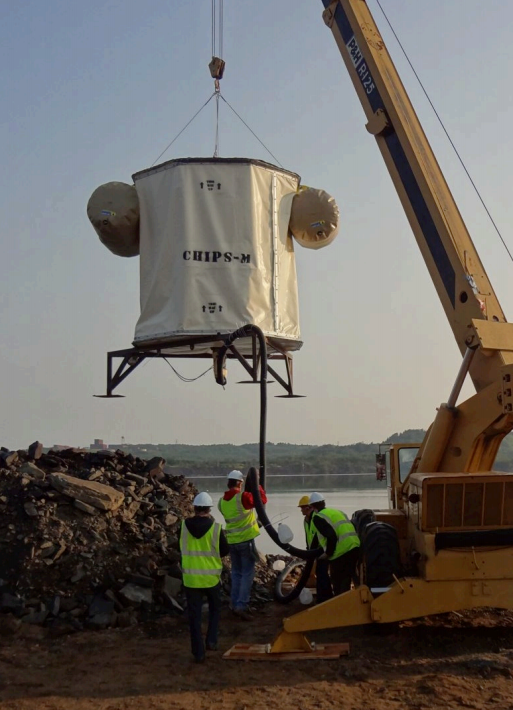
\includegraphics[width=0.6\textwidth]{diagrams/4-chips/chips_m.png}
    \caption[Picture of the \chipsm detector.]
    {Picture of the \unit{3.3}{\mathrm{m}} high \chipsm detector just before deployment. The
        temporary floatation bags are visibly attached to the top rim of the detector.
        Additionally, the umbilical cord carrying data, power, and filtered water is attached to
        the bottom of the detector.}
    \label{fig:chips_m}
\end{figure}

\subsection{The neutrino beam and off-axis alignment} %%%%%%%%%%%%%%%%%%%%%%%%%%%%%%%%%%%%%%%%%%%%
\label{sec:chips_concept_beam} %%%%%%%%%%%%%%%%%%%%%%%%%%%%%%%%%%%%%%%%%%%%%%%%%%%%%%%%%%%%%%%%%%%

\chips detectors will primarily study the appearance of $\nu_{e}$ oscillating from $\nu_{\mu}$
over a long-baseline. To generate a sufficient number of GeV scale $\nu_{\mu}$, a high-intensity
accelerator beam is required. Currently, only two such beams exist, the J-PARC based beam in Japan
used by the T2K experiment and the \numi beam in the USA used by \nova. Here we describe the
\numi~\cite{adamson2016} (Neutrinos at the Main Injection) beam as it is directly relevant to
current \chips efforts. However, it is essential to note that \chips detectors are designed to be
used in any neutrino beam, including the future \numi replacement, LBNF.

The \numi beam is an accelerator muon neutrino beam produced at Fermilab near Chicago in the USA.
Beginning operation in 2005 for the MINOS experiment, \numi was upgraded in 2013 to provide a
higher intensity and energy, principally to achieve a peak in neutrino energy near the
$\sim$\unit{1.5}{\GeV} $\nu_{\mu}\rightarrow\nu_{e}$ oscillation maximum for \nova. Currently the
\numi beam achieves an intensity above \unit{700}{\mathrm{kW}} (\unit{740}{\mathrm{kW}} peak)
making it the most powerful such beam in the world. A schematic of the \numi beamline
configuration is shown in Fig.~\ref{fig:numi_beam}.

\begin{figure} % NUMI BEAM DIAGRAM %
    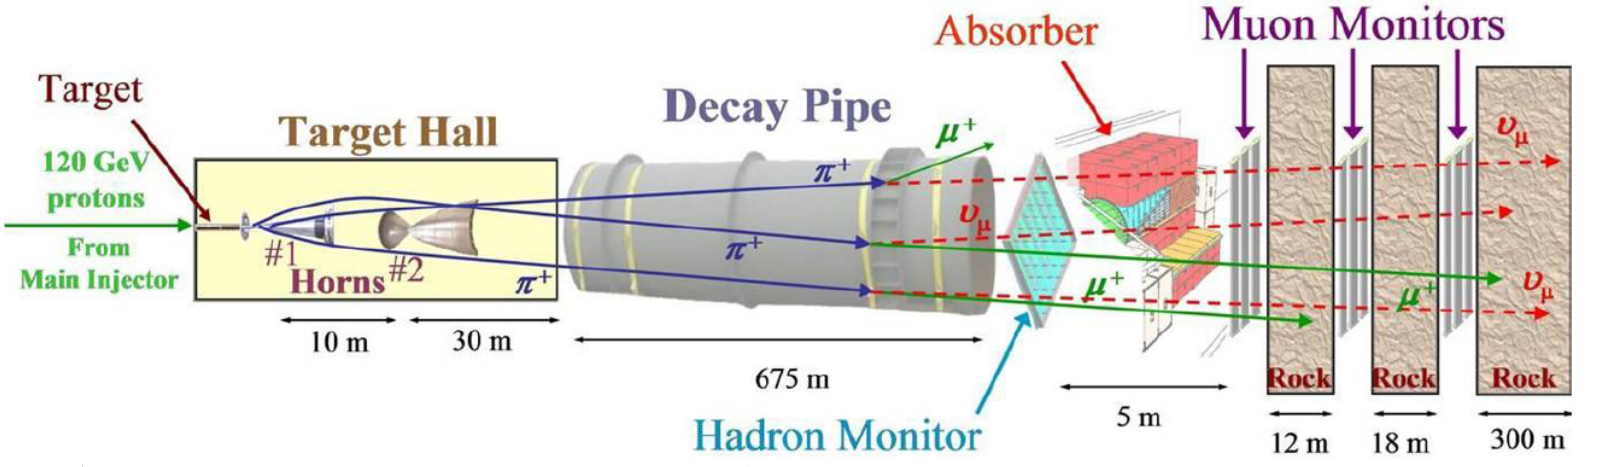
\includegraphics[width=\textwidth]{diagrams/4-chips/numi_beam.png}
    \caption[Schematic of the main components of the \numi beam.]
    {Schematic of the main components of the \numi beam (not to scale) shown with dimensions. The
        MINOS and \nova near detectors and the MINERvA experiment are located just to the right
        of what is shown. Figure taken from Ref.~\cite{adamson2016}.}
    \label{fig:numi_beam}
\end{figure}

Every \unit{1.33}{\mathrm{seconds}} a \unit{10}{\mu\mathrm{s}} long spill of protons accelerated
to \unit{120}{\GeV} by the Main Injector ring are directed towards a stationary graphite target.
The resulting interactions within the target create a shower of secondary hadrons containing
predominantly pions and kaons. The hadrons are passed through a focusing system of two magnetic
horns tuned principally to focus charged pions along the beamline while rejecting other particles.
After focusing, the surviving hadrons are allowed to decay in flight to a beam of muon neutrinos
in a \unit{675}{\mathrm{m}} long decay pipe via the processes,
\begin{align} % NUMI DECAY EQUATIONS %
    \pi^{+} & \rightarrow\mu^{+}+\nu_{\mu}, \label{eq:pi_decays}   \\
    K^{+}   & \rightarrow\mu^{+}+\nu_{\mu}. \label{eq:kaon_decays}
\end{align}
The resulting muons also decay such that $\mu^{+}\rightarrow e^{+}+\nu_{e}+\bar{\nu}_{\mu}$
producing an intrinsic $\nu_{e}$ background as well as wrong sign $\nu_{\mu}$ contamination.

Alternatively, the polarity of the horns can be used to switch the dominant sign of the hadrons
focused, allowing \numi to operate as either a neutrino or antineutrino beam. These two modes of
operation are called \emph{forward horn current} and \emph{reverse horn current} for primarily a
neutrino or antineutrino beam composition respectively. Any remaining hadrons, alongside
electrons, muons and surviving primary protons are absorbed by rock downstream of the decay pipe,
leaving just the neutrino components of the beam.

Long-baseline neutrino experiments typically consist of a \emph{near detector} to measure the beam
neutrino composition at source and a much larger \emph{far detector} to measure the oscillated
composition at many hundreds of kilometres. The \numi beamline contains three detectors just
downstream of \unit{300}{\mathrm{m}} of rock: The MINERvA spectrometer~\cite{mcfarland2006}, the
near detector for MINOS (now used by MINERvA), and the near detector for \nova. \chips prototypes
within the \numi beam will not have a dedicated near detector; therefore, data from the above
detectors will be crucial for physics analysis in order to constrain the beam composition and
flux.

The \numi neutrino beam passes through the Earth's crust until it finally emerges in northern
Minnesota. This is where the MINOS, \nova, and prototype \chips far detectors are located (used to
be located in the MINOS case), as shown in Fig.~\ref{fig:numi_map}. The Minnesota state nickname
`land of 10,000 lakes' is not an overstatement, with a vast number of potential lakes for \chips
detector deployment. Additionally, intense iron ore mining on the `Iron Range' provides many
suitable disused (and now flooded) mine pits. The exact \chipsfive prototype detector location is
discussed in greater detail in Section.~\ref{sec:chips_detector}.

\begin{figure} % CHIPS LOCATION IN NUMI DIAGRAM %
    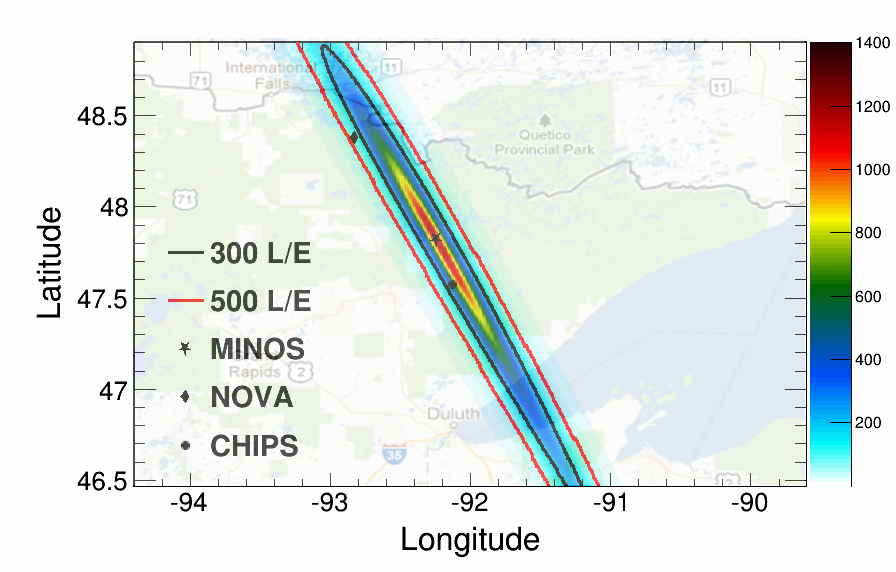
\includegraphics[width=0.7\textwidth]{diagrams/4-chips/numi_map.png}
    \caption[Map of detector locations in the \numi beam.]
    {Map of the MINOS, \nova and \chips locations in the \numi beam as it surfaces in northern
        Minnesota. Shown is the expected neutrino event rate assuming no oscillations, with lines
        of constant L/E indicated by contours. The western extent of Lake Superior can be seen in
        the lower right of the map. Image taken from Ref.\cite{adamson2013}.}
    \label{fig:numi_map}
\end{figure}

Due to the kinematics of pion decay, whether the far detector is placed directly on the beam axis
or not can have a significant impact on the observed energy spectrum of beam neutrinos as shown in
Fig.~\ref{fig:numi_axis}. For neutrinos directly on the beam axis, there is a strong energy
dependence on the parent pion energy from Eq.~\ref{eq:pi_decays}. However, as the off-axis angle
increases, the neutrino energy becomes less dependent on the parent pion energy and is restricted
to a narrowing range of decreasing energies. This effect known as the \emph{off-axis effect} is
used by both \nova and T2K to create a narrower energy spectrum focused on the
$\nu_{\mu}\rightarrow\nu_{e}$ oscillation maximum. Additionally, by reducing the tail of
higher-energy neutrinos, the number of background NC events can be greatly reduced, as is the case
for the \unit{7}{\mathrm{mrad}} off-axis \chipsfive prototype detector.

\begin{figure} % OFF-AXIS FLUX DIAGRAM %
    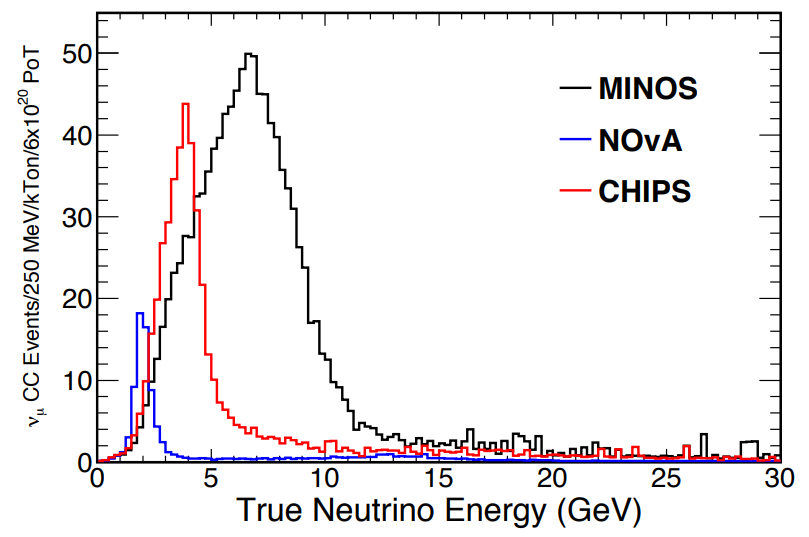
\includegraphics[width=0.6\textwidth]{diagrams/4-chips/numi_axis.png}
    \caption[Muon neutrino flux for different \numi detectors at different off-axis angles.]
    {Muon neutrino flux for different \numi detectors at different off-axis angles. Shown are the
        neutrino energy spectrum for MINOS (on-axis), \nova (\unit{14}{\mathrm{mrad}} off-axis),
        and \chipsfive (\unit{7}{\mathrm{mrad}} off-axis). Figure taken from
        Ref.~\cite{adamson2013}.}
    \label{fig:numi_axis}
\end{figure}

\subsection{Water Cherenkov detectors} %%%%%%%%%%%%%%%%%%%%%%%%%%%%%%%%%%%%%%%%%%%%%%%%%%%%%%%%%%%
\label{sec:chips_concept_cherenkov} %%%%%%%%%%%%%%%%%%%%%%%%%%%%%%%%%%%%%%%%%%%%%%%%%%%%%%%%%%%%%%

The \chips detector concept is based upon the water Cherenkov technique for neutrino detection. A
large body of target water is instrumented with photomultiplier tubes (PMTs) to record the
Cherenkov radiation produced by sufficiently relativistic charged particles resulting from
neutrino interactions. By using readily available water as the target material and only
instrumenting the volume surface, water Cherenkov detectors provide the best detection methodology
for maximising volume and reducing cost.

Cherenkov radiation is emitted by all electrically charged particles travelling faster than the
local phase velocity of light in a dielectric medium. Similar to the sonic boom created by a
supersonic aircraft, Cherenkov radiation forms a shock wave of coherent light, as shown in
Fig.~\ref{fig:cherenkov}. Typically the emitted light has wavelengths in the optical to
ultraviolet range. When projected onto the detector wall, the resulting cone of radiation
generates a distinctive ring shape. The cone opening angle (the angle at which light is emitted)
$\theta_{c}$ is given by:
\begin{equation}
    \cos\theta_{c} = \frac{1}{\beta n(\lambda)},
    \label{eq:cherenkov_angle}
\end{equation}
where $\beta=v/c$ and $n$ is the refractive index of the medium~\cite{particle2020}. Note that $n$
is a function of the wavelength of emission $\lambda$, and so is the opening angle. As the
refractive index of water is $\sim 1.33$ for typical wavelengths of emission, and using the
ultrarelativistic limit $\beta\sim 1$ the opening angle is found to be $\sim41^{\circ}$.

\begin{figure} % CHERENKOV EFFECT DIAGRAM DIAGRAM %
    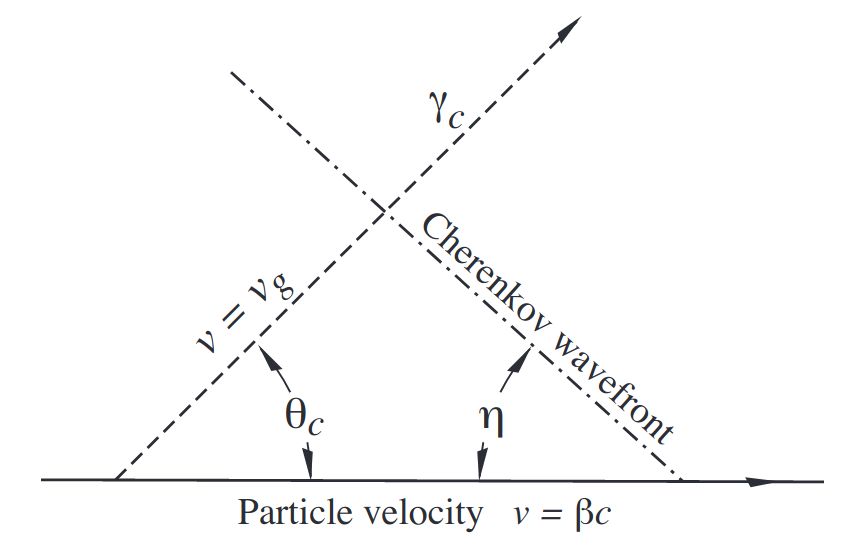
\includegraphics[width=0.6\textwidth]{diagrams/4-chips/cherenkov.png}
    \caption[Diagram of Cherenkov radiation emission.]
    {Diagram of Cherenkov radiation emission and wavefront angles. The angles $\theta_{c}$ and
        $\eta$ are not equal in a dispersive medium. Figure taken from Ref.~\cite{particle2020}}
    \label{fig:cherenkov}
\end{figure}

In Eq.~\ref{eq:cherenkov_angle} there is no Cherenkov emission when $\cos\theta_{c} > 1$, which is
the case when $\beta n(\lambda)<1$. Therefore, a Cherenkov energy threshold $E_{t}$ exists for
charged particle, which when expressed in terms of the particle mass $m$ is given by:
\begin{equation}
    E_{t} = \gamma m = \frac{m}{\sqrt{1-(1/n)^{2}}}.
    \label{eq:cherenkov_threshold}
\end{equation}
Again using $n\sim 1.33$, a threshold energy of $\sim1.5m$ is typical.

The number of Cherenkov photons emitted by a particle of charge $ze$ per unit wavelength per unit
path length is given by:
\begin{equation}
    \frac{d^{2}N}{d\lambda dx}=\frac{2\pi\alpha z^{2}}{\lambda^{2}}
    \left(1-\frac{1}{1-\beta^{2}n^{2}(\lambda)}\right),
    \label{eq:cherenkov_emission}
\end{equation}
where $\alpha$ is the fine structure constant~\cite{particle2020}. Integrating over the range of
wavelengths for which PMTs are typically sensitive, \unit{350}{\mathrm{nm}} to
\unit{650}{\mathrm{nm}}, and using $\beta\sim 1$ and $n\sim 1.33$ gives $\sim240$ photons emitted
per cm travelled by the charged particle~\cite{perch2017}.

By analysing the Cherenkov ring (or rings) of light recorded by the PMTs on the walls of the
detector, information about the charged particle (particles) within an event can be determined.
The underlying neutrino interaction can then be understood indirectly. Primarily the challenge for
accelerator beam water Cherenkov detectors is the identification and reconstruction of an electron
or muon ring likely to have been produced from a beam neutrino and not a cosmic ray. This event
topology indicates a beam CC $\nu_{e}$ or CC $\nu_{\mu}$ event respectively, rejecting NC and
cosmic events.

The basic shape of a Cherenkov ring can be used to tell which charged particle created it. Muons
are long-lived and typically travel many metres within the detector, producing a clean ring with
sharp edges. Conversely, electrons almost immediately initiate an electromagnetic shower;
therefore, the observed ring is the sum of all the rings produced from the individual electrons
and positrons within the shower. As a consequence, when compared to a muon ring, electron rings
are characteristically fuzzy. A factor of this difference can be seen in Fig.~\ref{fig:emission
    distance}, which shows how the total amount of Cherenkov radiation is emitted for both electrons
and muons as a function of distance from the interaction vertex.

\begin{figure} % EMISSION DISTANCE DIAGRAM %
    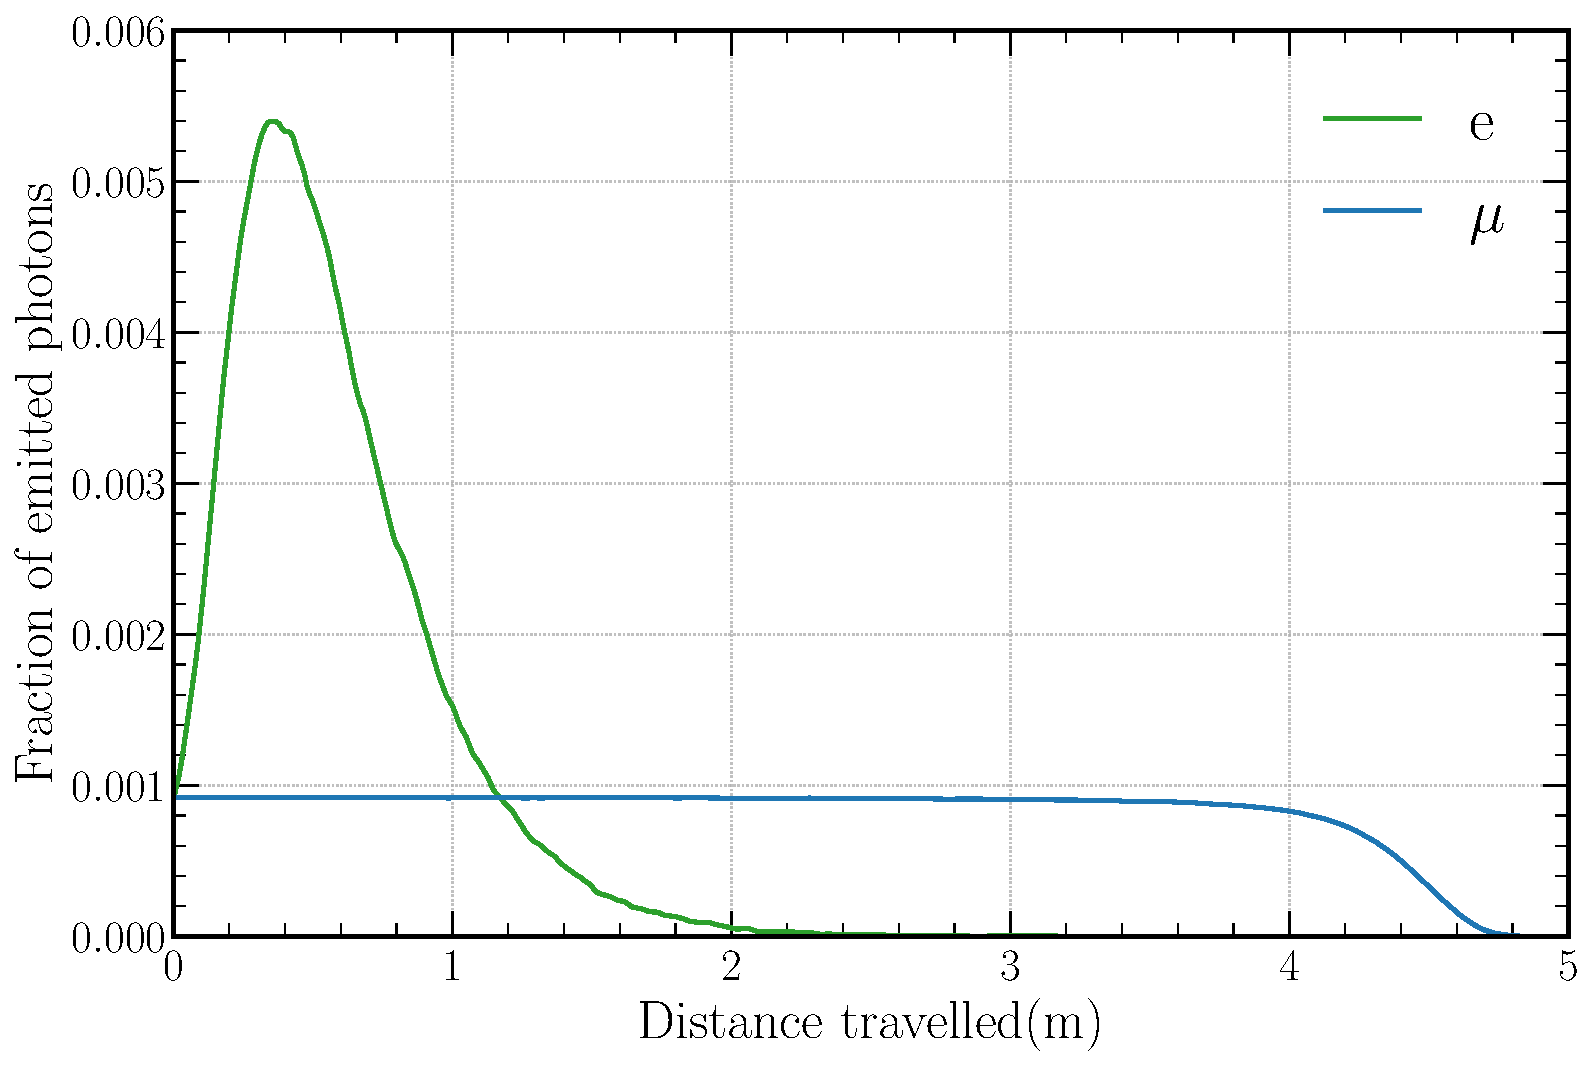
\includegraphics[width=0.6\textwidth]{diagrams/4-chips/emission_distance.pdf}
    \caption[Fraction of Cherenkov photons emitted as a function of distance.]
    {The fraction of the total number of photons emitted as a function of the distance from the
        interaction vertex for both electrons and muons with energy of \unit{2.5}{\GeV}. Multiple
        particles within the electron induced electromagnetic shower emit their Cherenkov
        radiation over a short distance and in slightly different directions. Conversely, a muon
        travels relatively much further emitting an approximately constant level of Cherenkov
        radiation as it does so, leading to a clean, sharp-edged ring.}
    \label{fig:emission distance}
\end{figure}

The situation becomes complicated when multiple charged particles above the Cherenkov threshold
are involved, common at multi-$\GeV$ energies. In this case, multiple overlapping rings are
observed, making reconstruction difficult. The worst-case scenario, however, is when two rings
entirely overlap, removing any ability to tell them apart. This topology is commonly the case for
NC interactions producing a $\pi^{0}$ in the final state, forming the primary background for CC
$\nu_{e}$ appearance.

$\pi^{0}$ particles decay to a pair of photons with a 98.82\% branching ratio, both which almost
immediately initiate an electromagnetic shower, just like an electron~\cite{particle2020}. This
process leads to two, electron like rings to be observed with a separation angle given by:
\begin{equation}
    (1-\cos\theta_{ij})=\frac{m_{\pi}^2}{2E_{i}E_{k}},
\end{equation}
where $m_{\pi}$ is the invariant mass of the $\pi^{0}$ and $E_{i}$ and $E_{j}$ are the energies of
the two photons respectively. Therefore, for a $\pi^{0}$ decaying to two \unit{1}{\GeV} photons,
there is just $\sim 8^{\circ}$ of separation between the rings, making them difficult to tell
apart. This distinction is especially hard when electron like rings are also fuzzy. Alternatively,
if the two photons have an unequal energy distribution, such that one is much more energetic than
the other, the higher energy photon ring can dominate, and the other can not be identified,
leading to what looks like a single electron ring, again a misidentification.

\section{The \chipsfive detector} %%%%%%%%%%%%%%%%%%%%%%%%%%%%%%%%%%%%%%%%%%%%%%%%%%%%%%%%%%%%%%%%
\label{sec:chips_detector} %%%%%%%%%%%%%%%%%%%%%%%%%%%%%%%%%%%%%%%%%%%%%%%%%%%%%%%%%%%%%%%%%%%%%%%

\chipsfive is the first large scale prototype detector module for the \chips project. A
\unit{25}{\mathrm{m}} wide and \unit{12}{\mathrm{m}} high cylinder once fully deployed, \chipsfive
has an inner surface area of \unit{1924}{\mathrm{m}^2} and a total target mass
\unit{5.9}{\mathrm{kton}}. Via the process of design, construction, deployment, and data taking,
\chipsfive primarily aims to refine the \chips concept for future full-scale
($\sim$\unit{15}{\mathrm{kton}}) modules. Consequently, \chipsfive is designed such that the
details outlined in this section are fully characteristic of what a full-sized \chips module is
envisioned to be. Here, the location, structure, instrumentation, water filtration, deployment,
and current status are presented. The full electronics and DAQ details are outlined in
Chapter.~\ref{chap:daq}.

\subsection{Location} %%%%%%%%%%%%%%%%%%%%%%%%%%%%%%%%%%%%%%%%%%%%%%%%%%%%%%%%%%%%%%%%%%%%%%%%%%%
\label{sec:chips_detector_location} %%%%%%%%%%%%%%%%%%%%%%%%%%%%%%%%%%%%%%%%%%%%%%%%%%%%%%%%%%%%%

\chipsfive is located at the Wentworth 2W pit in northern Minnesota, USA, near the small town of
Hoyt Lakes. A disused and flooded surface Taconite ore (a type of iron ore) mine pit, Wentworth 2W
is located \unit{7}{\mathrm{mrad}} off the \numi axis at a distance of \unit{712}{\mathrm{km}}
from the beam target. Roughly \unit{0.8}{\mathrm{km}}$\times$\unit{1.2}{\mathrm{km}} in size with
a maximum depth of \unit{60}{\mathrm{m}} ($\pm3\mathrm{m}$ throughout the year), the pit allows
for an overburden of approximately \unit{50}{\mathrm{m}} with \chipsfive resting at the bottom.
With an average daily low temperate of $-24^{\circ}\mathrm{C}$ in January, the pit freezes over
during the winter months, therefore, work is only possible during the summer months of May to
October.

A sizeable earthen ramp on the south side of the Wentworth 2W pit is used for construction on
land. The construction site is easily accessible by road and well connected to power, due to the
heavy infrastructure in place for mining. Additionally, the nearby PolyMet mining administration
building is used as a laboratory environment for construction and testing of individual components
before installation within the detector. A labelled satellite view of Wentworth 2W is given in
Fig.~\ref{fig:pit} for context, with a picture of the construction site shown in
Fig.~\ref{fig:from_the_sky}.

\begin{figure} % PIT DIAGRAM %
    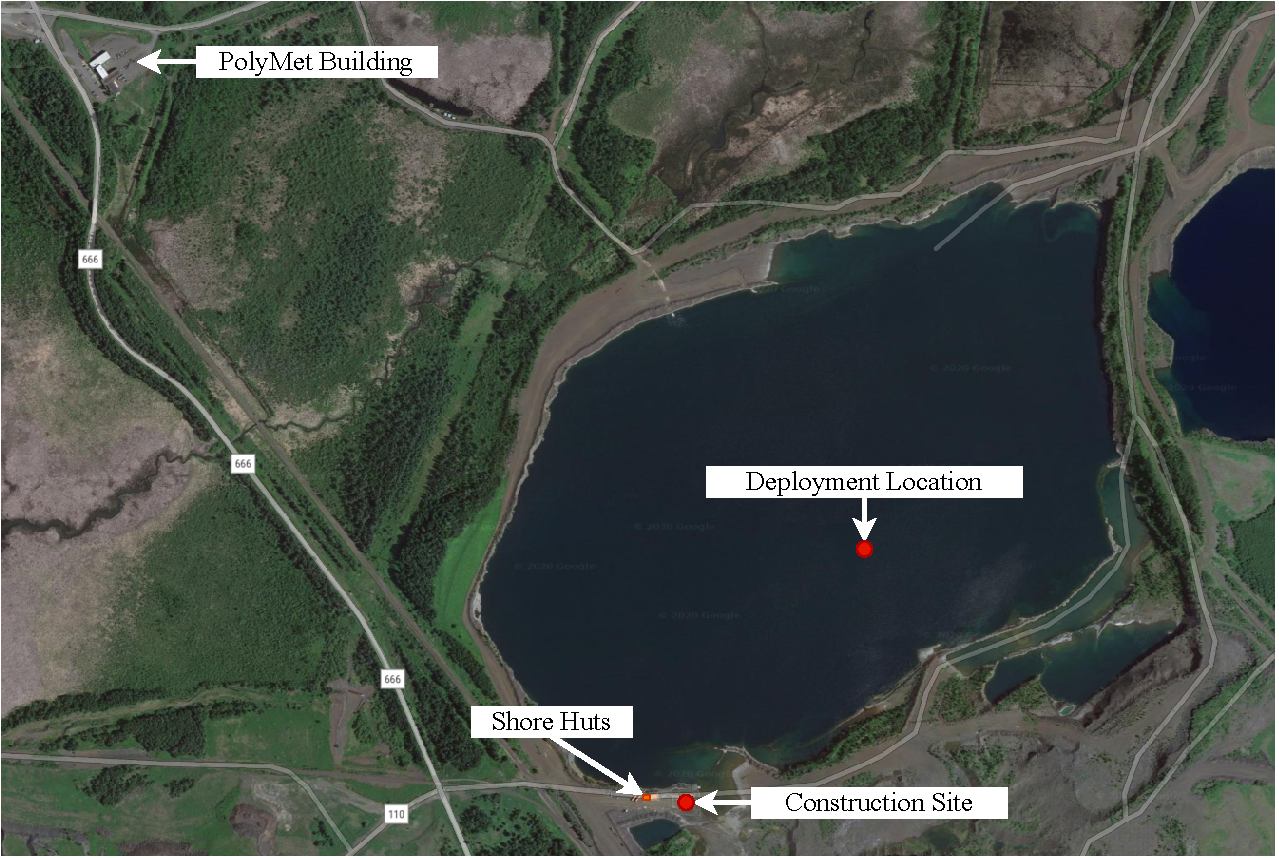
\includegraphics[width=\textwidth]{diagrams/4-chips/pit.pdf}
    \caption[Satellite view of the Wentworth 2W mine pit, with key locations.]
    {Satellite view of the Wentworth 2W flooded mine pit in northern Minnesota, showing key
        \chipsfive locations. The PolyMet building, shore huts, construction site and deployment
        location are shown. For both the construction site and deployment location the red circle
        shows the \chipsfive detector size to scale.}
    \label{fig:pit}
\end{figure}

\begin{figure} % CHIPS FROM THE SKY DIAGRAM %
    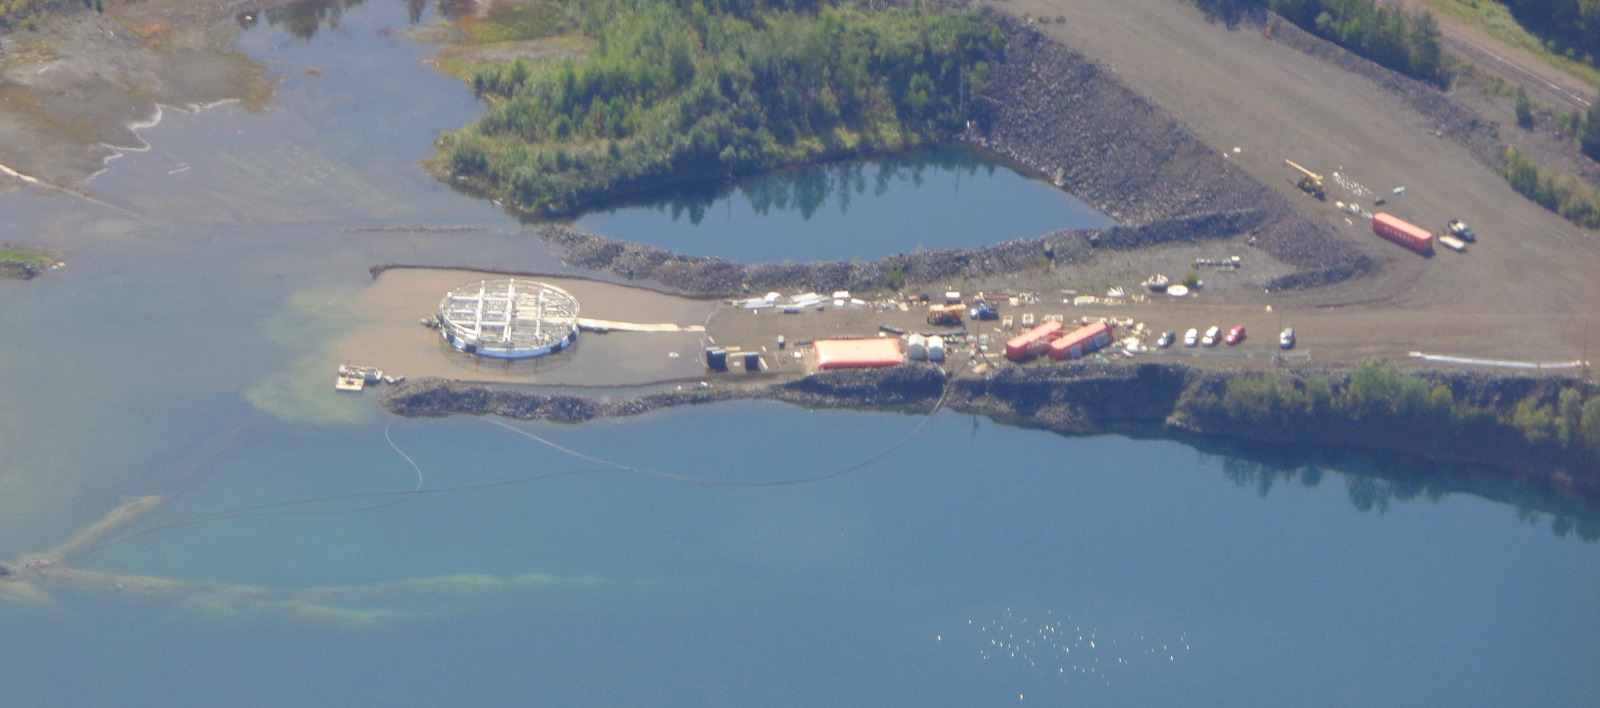
\includegraphics[width=\textwidth]{diagrams/4-chips/from_the_sky.jpg}
    \caption[Picture of the \chipsfive construction site from the air.]
    {Picture of the \chipsfive construction site from the air facing south. The Wentworth 2W pit
        is in the lower half of the image, with the part built \chipsfive detector visible at the
        bottom of the earthen construction ramp. The two white shore huts can just be seen halfway
        up the ramp.}
    \label{fig:from_the_sky}
\end{figure}

\subsection{Structure} %%%%%%%%%%%%%%%%%%%%%%%%%%%%%%%%%%%%%%%%%%%%%%%%%%%%%%%%%%%%%%%%%%%%%%%%%%%
\label{sec:chips_detector_structure} %%%%%%%%%%%%%%%%%%%%%%%%%%%%%%%%%%%%%%%%%%%%%%%%%%%%%%%%%%%%%

The structure of the \chipsfive detector module consists primarily of two \unit{26}{\mathrm{m}}
diameter and \unit{1.3}{\mathrm{m}} high lightweight stainless steel circular \emph{endcaps} that
form the top and bottom of the cylinder. During construction on land the conveniently named
\emph{top-cap} is held above the \emph{bottom-cap} by \unit{1.5}{\mathrm{m}} long steel struts as
shown in Fig.~\ref{fig:frame}. This configuration allows for the endcap instrumentation, detailed
in Section.~\ref{sec:chips_detector_instrumentation}, to be easily installed.

\begin{figure} % CHIPS FRAME DIAGRAM %
    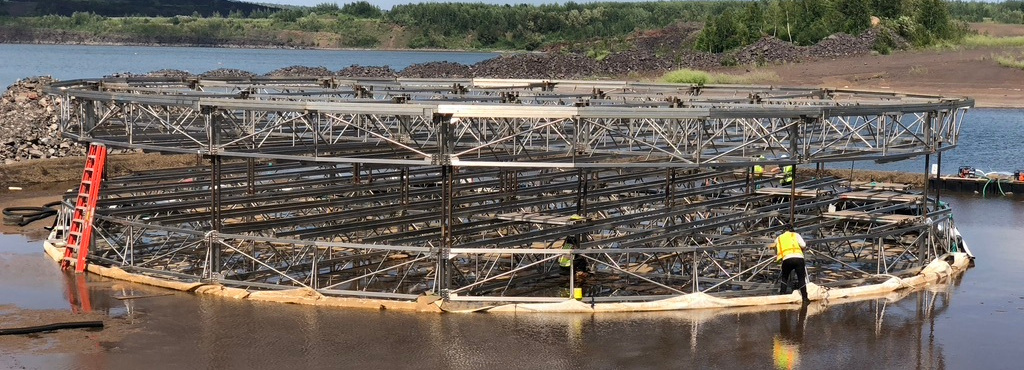
\includegraphics[width=\textwidth]{diagrams/4-chips/frame.jpeg}
    \caption[Picture of the \chipsfive structural frame.]
    {Picture of the \chipsfive structural frame, with humans for scale. The top and bottom endcaps
        can be seen separated by steel struts. Rows of stainless steel \emph{stringers}
        are attached to the inside of each endcap to mount the instrumentation.}
    \label{fig:frame}
\end{figure}

The two endcaps are connected by 28 \unit{12}{\mathrm{m}} long Dyneema cables around their
perimeter. Additionally, 48 \unit{16}{\mathrm{inch}} diameter air-filled PVC pipes are attached to
the frame of the top-cap, making it buoyant. Therefore, once deployed into the pit, the bottom-cap
sinks while the top-cap floats, this pulls the Dyneema cable until taut, forming the final
expanded detector shape, as shown in Fig.~\ref{fig:chips_render}.

\begin{figure} % CHIPS RENDER DIAGRAM %
    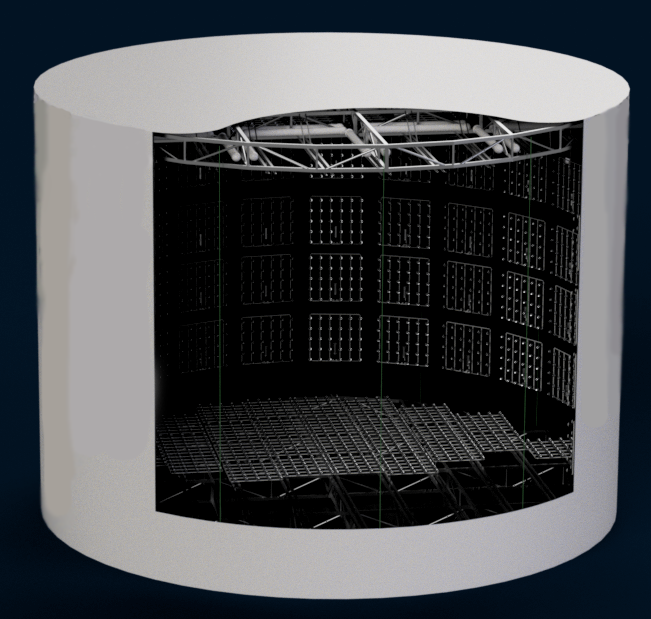
\includegraphics[width=0.6\textwidth]{diagrams/4-chips/chips_render_1.png}
    \caption[Graphical rendering of the \chipsfive detector.]
    {Graphical rendering of the fully deployed and expanded \chipsfive detector module with a
        section of the liner cutaway. The bottom endcap and wall planes are visible, as well as
        the top endcap structure and floatation. The green lines indicate the Dyneema cables
        holding the top-cap and bottom-cap together.}
    \label{fig:chips_render}
\end{figure}

A lightproof and watertight liner is also installed to surround the fully expanded structure.
Designed to isolate the clean internal water from the external pit water and to prevent
non-Cherenkov light from reaching the PMTs, the liner is made from geomembrane, a flexible
reinforced polymer membrane. Commercially available in large rolls the liner is welded together
during construction to form the top, bottom, and sides. Note that when fully deployed, the liner
does not take any of the structural strain.

\subsection{Instrumentation} %%%%%%%%%%%%%%%%%%%%%%%%%%%%%%%%%%%%%%%%%%%%%%%%%%%%%%%%%%%%%%%%%%%%%
\label{sec:chips_detector_instrumentation} %%%%%%%%%%%%%%%%%%%%%%%%%%%%%%%%%%%%%%%%%%%%%%%%%%%%%%%

The \chipsfive detector is instrumented with PMTs arranged within distinct plane like structures
called Planar Optical Modules (POMs), which take inspiration from the Digital Optical Modules
(DOMs) used by IceCube and KM3NeT~\cite{hanson2006, eijk2015}. Each POM is a roughly
\unit{2}{\mathrm{m}}$\times$\unit{3}{\mathrm{m}} array of watertight PVC tubing equipped with
anywhere between $15$ to $30$ PMTs, in addition to the lowest level of DAQ electronics and power
distribution. Standard commercially available schedule $40$ PVC piping and connectors are used to
form the structure of each plane, bound together with PVC primer and cement.

There are two types of POM used within \chipsfive, differentiated by the PMTs and the data
acquisition electronics they use and named after the institution at which they were developed.
Firstly, \emph{Nikhef} POMs use \unit{88}{\mathrm{mm}} HZC PMTs with electronics developed by the
KM3NeT experiment~\cite{katz2009, adrian2016}. Secondly, \emph{Madison} POMs use
\unit{3}{\mathrm{inch}} Hamamatsu R6091 PMTs donated from the NEMO3 experiment~\cite{arnold2005}
with novel electronics developed by \chips in collaboration with the Wisconsin IceCube Particle
Astrophysics Centre (WIPAC) in Madison, Wisconsin. The \unit{88}{\mathrm{mm}} HZC PMTs have a high
ratio of output electrons to incident photons (quantum efficiency) of 24.4\% at a wavelength of
\unit{400}{\mathrm{nm}}, compared to the low 12.0\% ratio achieved by the R6091 PMTs. Furthermore,
the first photon time resolution is $\sim2\mathrm{ns}$ and $\sim5\mathrm{ns}$ for
\unit{88}{\mathrm{mm}} HZC and R6091 PMTs respectively.

In total $6114$ \unit{88}{\mathrm{mm}} HZC and $450$ Hamamatsu R6091 PMTs are arranged into $226$
Nikhef and $30$ Madison POMs. Every PMT is housed in an assembly as shown in
Fig.~\ref{fig:nikhef_pmt_assembly} for the Nikhef case and Fig.~\ref{fig:madison_pmt_assembly} for
the Madison case. Importantly, to increase the level of light collection, each Nikhef PMT is
equipped with a \emph{light-cone} consisting of a circular reflective surface at \unit{45}{^\circ}
to the PMT normal. The Madison PMT assembly is similar but has no cover or light cone. For POMs
attached to either endcap, their PMTs are angled at \unit{45}{^\circ} facing the direction of the
beam to increase light collection furthermore.

All PMTs within a POM are connected to the lowest level of DAQ electronics contained within a
dedicated electronics box. Either an aluminium or PVC cylinder in the Nikhef or Madison case
respectively. A flexible PVC \emph{pigtail} is attached to each POM electronics box containing
connections to the higher level DAQ and power supply. A \emph{water-block} within each pigtail
ensures that even if the outside connection is flooded, every POM is capable of withstanding the
\unit{6}{\mathrm{atm}} of water pressure at the bottom of the pit. A fully assembled and installed
Nikhef POM is shown in Fig.~\ref{fig:single_plane} for reference.

\begin{figure} % NIKHEF PMT ASSEMBLY DIAGRAM %
    \centering
    \subcaptionbox{Disassembled}{%
        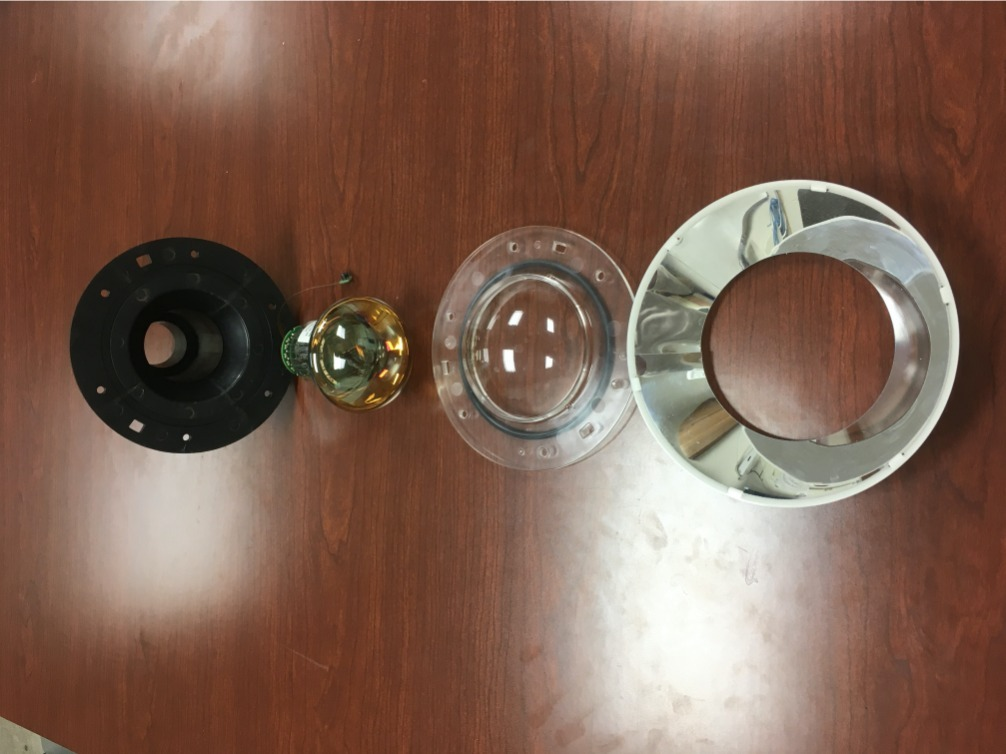
\includegraphics[height=5.5cm]{diagrams/4-chips/pmt_disassembled.jpg}%
    }
    \quad
    \subcaptionbox{Assembled}{%
        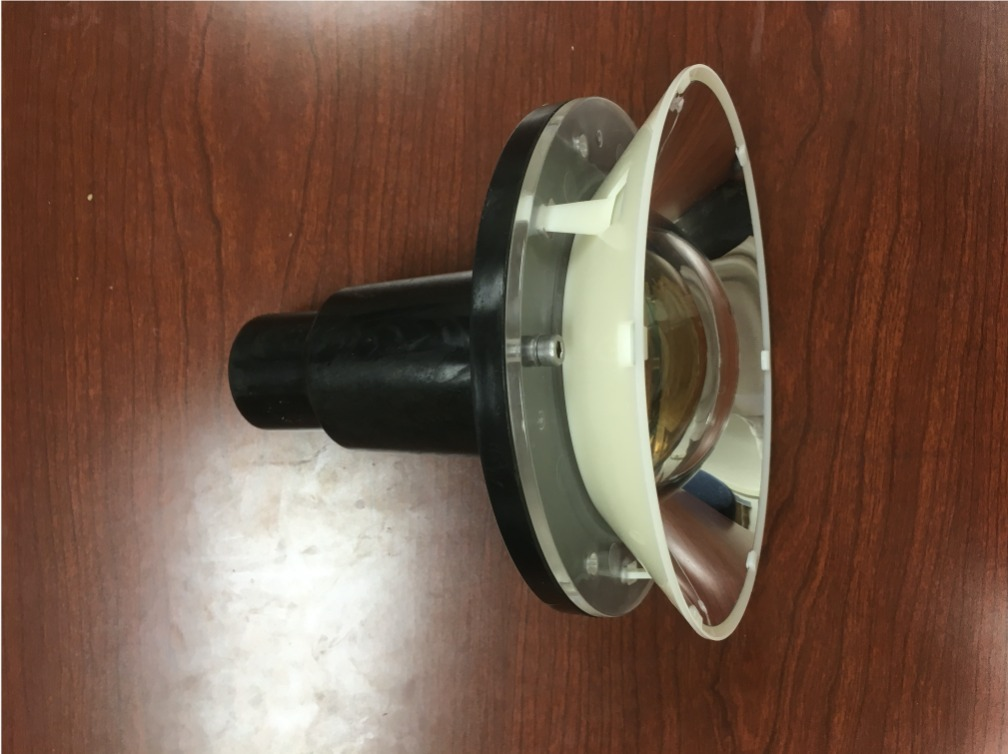
\includegraphics[height=5.5cm]{diagrams/4-chips/pmt_assembled.jpg}%
    }
    \caption[Disassembled and assembled Nikhef PMT housing components.]
    {Disassembled (a) and assembled (b) Nikhef PMT assembly components. The assembly comprises of
        a black PVC insert, a \unit{88}{\mathrm{mm}} HZC PMT, a transparent acrylic cover, and a
        reflective light cone. The PMT is glued to the inside surface of the cover using a
        silicone-based optical gel and a watertight seal is made between the insert and cover
        using an O-ring. The reflective light cone is clipped to the front of the cover and the
        whole assembly is glued into the POM PVC structure.}
    \label{fig:nikhef_pmt_assembly}
\end{figure}

\begin{figure} % MADISON PMT ASSEMBLY DIAGRAM %
    \centering
    \subcaptionbox{Outside}{%
        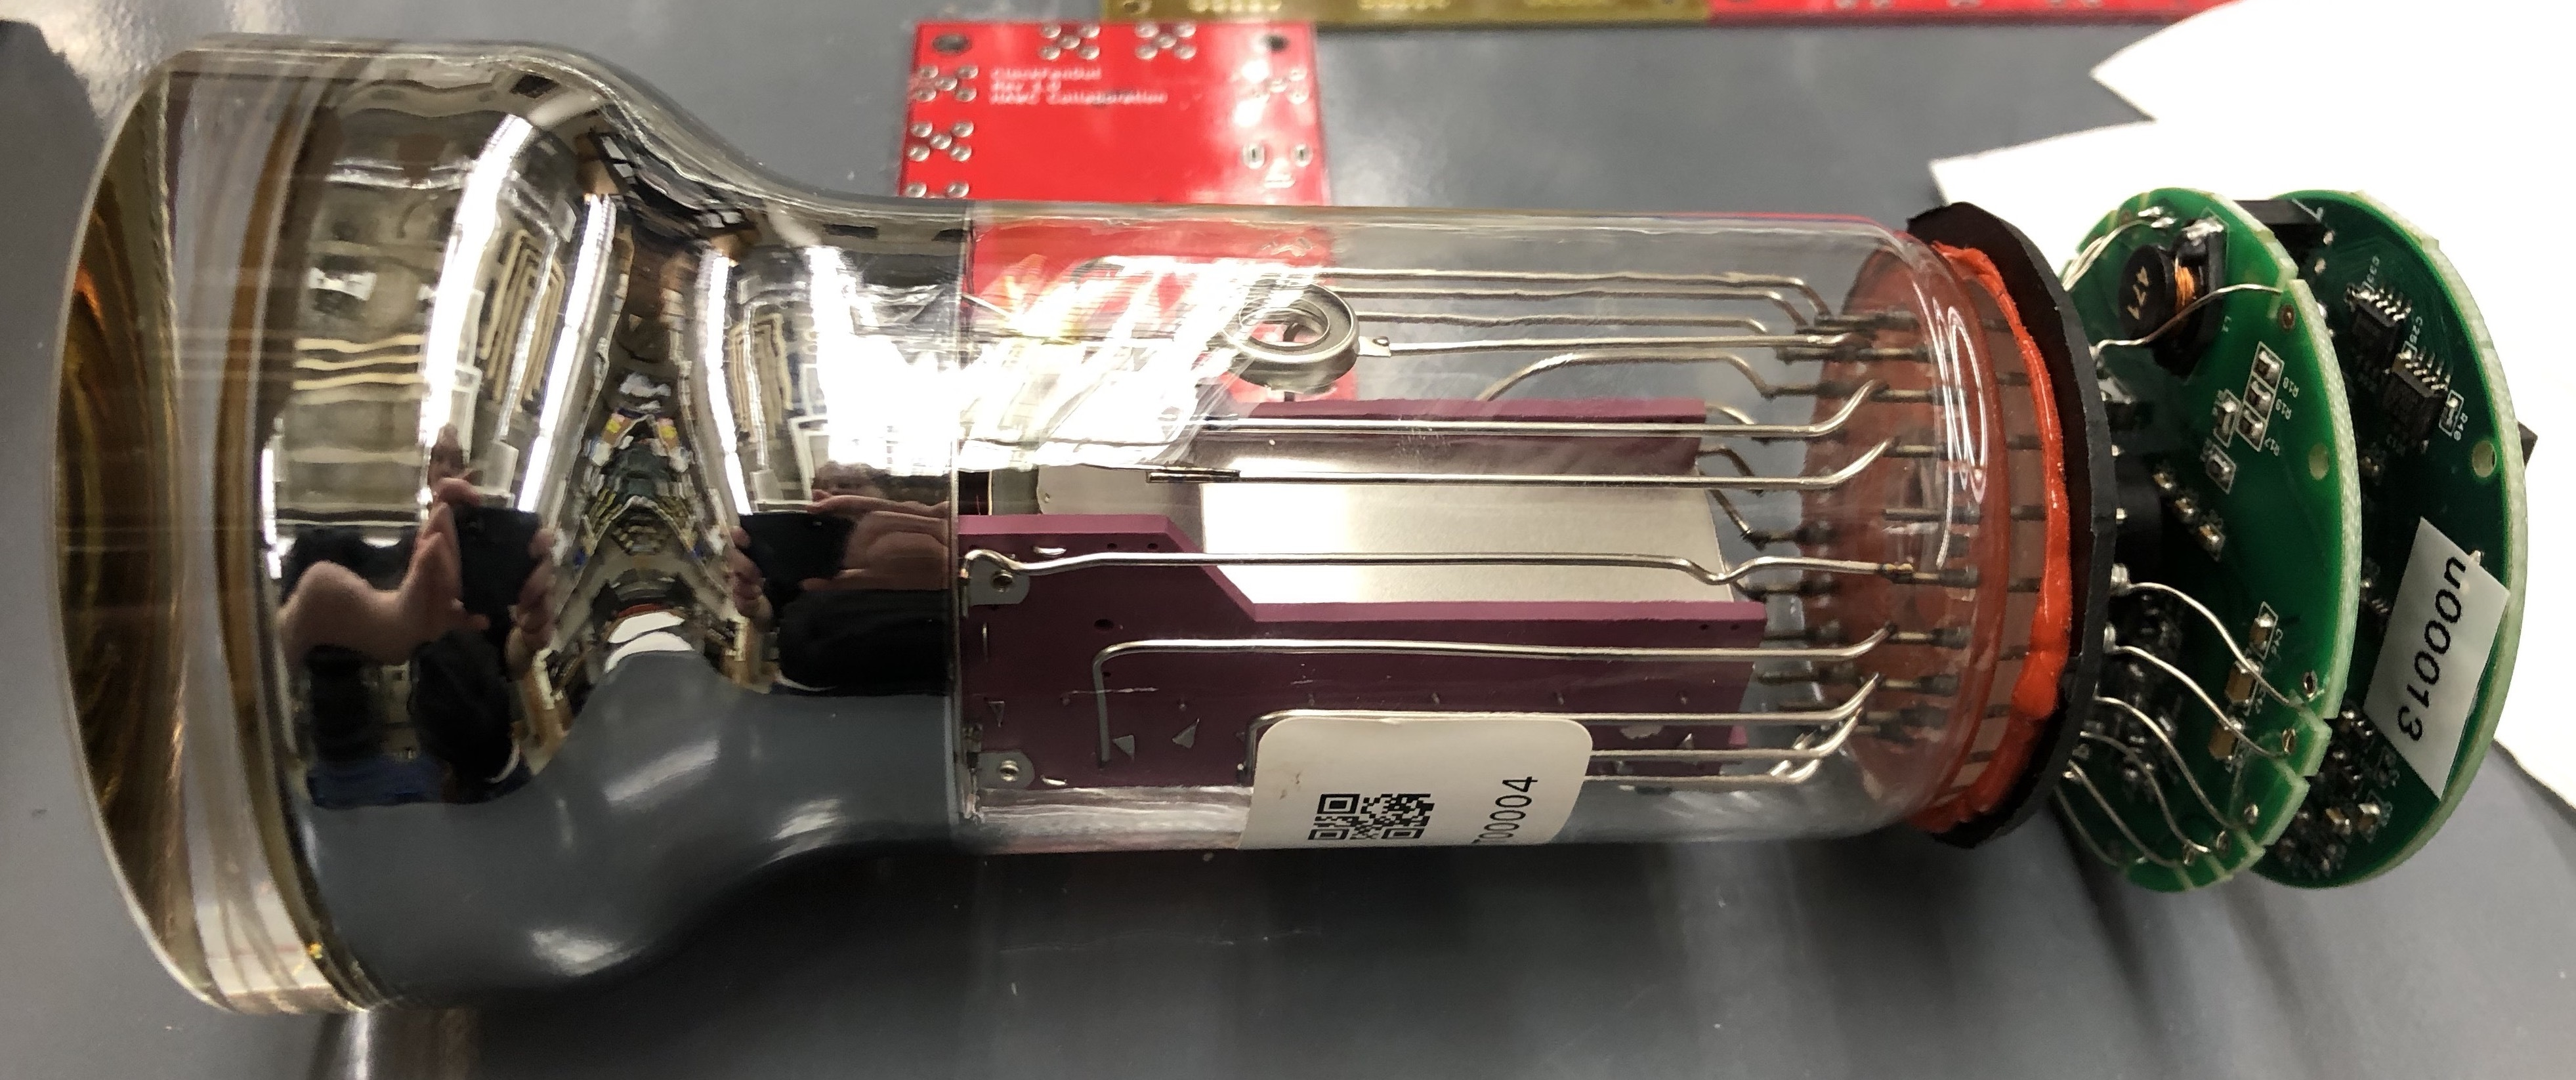
\includegraphics[angle=270,origin=c,height=4.3cm]{diagrams/4-chips/madison_pmt.jpeg}%
    }
    \quad
    \subcaptionbox{Inside}{%
        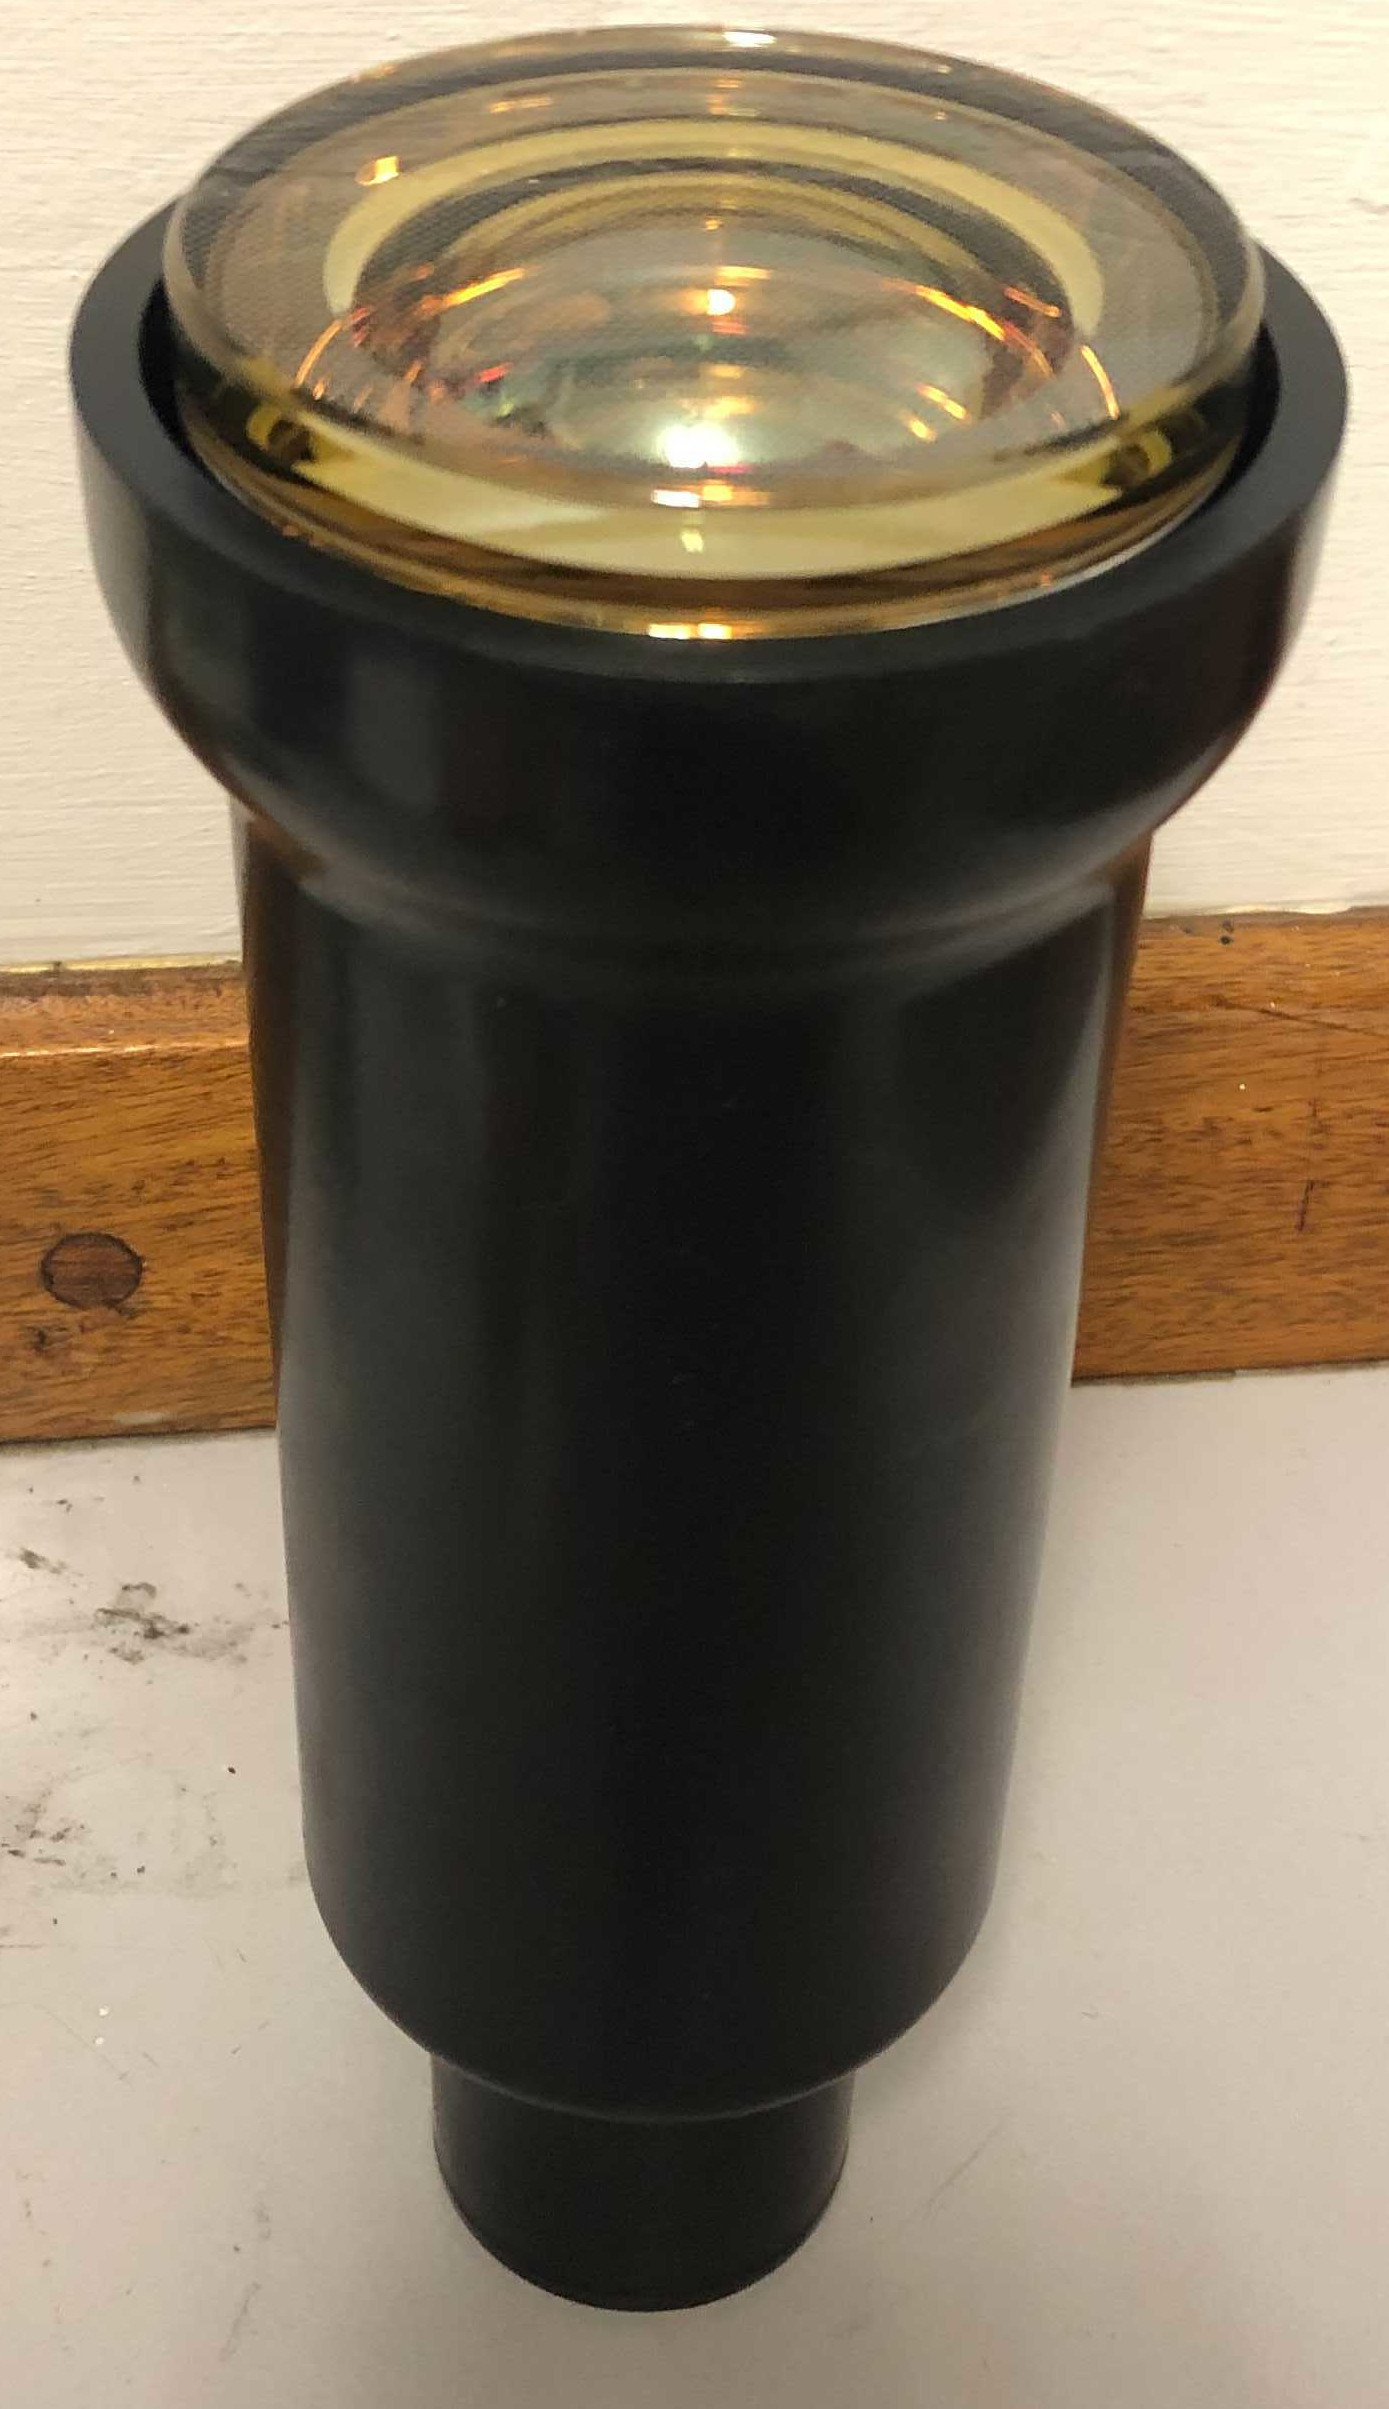
\includegraphics[height=6cm]{diagrams/4-chips/madison_assembly.jpg}%
    }
    \caption[Madison POM PMT assembly.]
    {A Hamamatsu R6091 Madison POM PMT outside (a) and inside its insert (b). The PMT is
        \emph{potted} inside its black PVC insert creating a watertight seal that can withstand the
        \unit{6}{\mathrm{atm}} of water pressure at the bottom of the pit.}
    \label{fig:madison_pmt_assembly}
\end{figure}

\begin{figure} % NIKHEF POM DIAGRAM %
    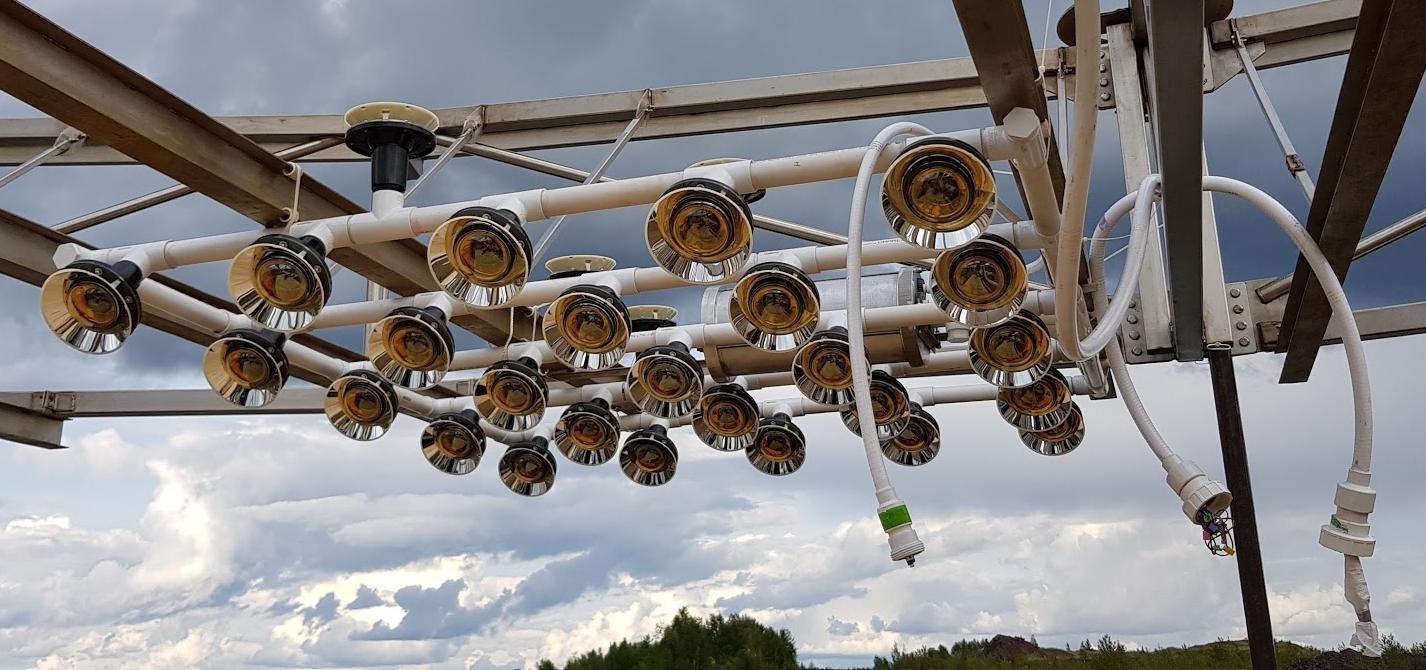
\includegraphics[width=\textwidth]{diagrams/4-chips/single_plane.jpg}
    \caption[Picture of a Nikhef POM.]
    {Picture of a single Nikhef full density POM installed on the top-cap of the \chipsfive
        detector. Both the inward-facing and veto PMTs are visible as well as the aluminium
        electronics container and pigtail whose end is covered in green tape.}
    \label{fig:single_plane}
\end{figure}

The POMs are tiled next to each other on the detector walls, attached to either the stainless
steel \emph{stringers} on the top-cap and bottom-cap, or clipped to the Dyneema cables on the
vertical walls of the \emph{barrel}. As mentioned previously, full high density and high coverage
detector instrumentation is not required for \chips detector modules, due to two main reasons.
Firstly, only highly directional accelerator beam events are to be studied. Therefore, the vast
majority of neutrino interaction Cherenkov radiation is deposited on a relatively small downstream
region of the detector walls. Secondly, beam neutrinos predominantly have multi-$\GeV$ energies,
yielding a relatively large amount of Cherenkov radiation. Therefore, a lower number of PMTs is
required to capture adequate Cherenkov radiation from an interaction.

Consequently, the distribution of the percentage of the detector walls covered by sensitive PMT
surface area (\emph{photocathode coverage}) is optimised to reduce the total number of PMTs. The
detector is split into three distinct regions of PMT photocathode coverage whose boundaries are
roughly defined by their azimuth angle $\phi$ from the centre of the downstream wall (at
$\phi=0^{\circ}$). Firstly, a \emph{full-density} Nikhef POM region in the most downstream
$\phi=\pm75^{\circ}$ region of the detector with a $\sim3\%$ photocathode coverage. Secondly, a
\emph{half-density} Nihkef POM region covering the $\phi=\pm75^{\circ}$ to $\phi=\pm180^{\circ}$
region of the endcaps and the $\phi=\pm75^{\circ}$ to $\phi=\pm140^{\circ}$ region of the barrel
with a $\sim1.5\%$ photocathode coverage. Finally, a \emph{half-density} Madison POM region
covering the $\phi=\pm140^{\circ}$ to $\phi=\pm180^{\circ}$ upstream region of the barrel with a
$\sim0.8\%$ photocathode coverage. Studies have shown that this configuration does not reduce
performance while vastly reducing the number of required PMTs~\cite{blake2016}.

Compared to the $\sim40\%$ uniform photocathode coverage of Super-Kamiokande, the \chipsfive
instrumentation configuration highlights just how significantly different detector design can be
when only studying accelerator beam neutrinos. Of importance to note is that photocathode coverage
in the upstream regions of the detector is still required, even if very low, for cosmic muon and
NC event rejection.

To further help with cosmic muon rejection, the \chipsfive detector module is equipped with a veto
region within the top-cap frame structure. Separated from the main detector volume by a
geomembrane liner, the \unit{1.3}{\mathrm{m}} high region can reject predominantly downward cosmic
muons by detecting the Cherenkov radiation they produce. $324$ \unit{88}{\mathrm{mm}} HZC PMTs are
included within the Nikhef POMs attached to the top-cap facing upwards leading to a veto
photocathode coverage of $\sim0.6\%$. A graphical rendering of all the top-cap POMs is shown in
Fig.~\ref{fig:top_cap}.

\begin{figure} % TOP CAP RENDER DIAGRAM %
    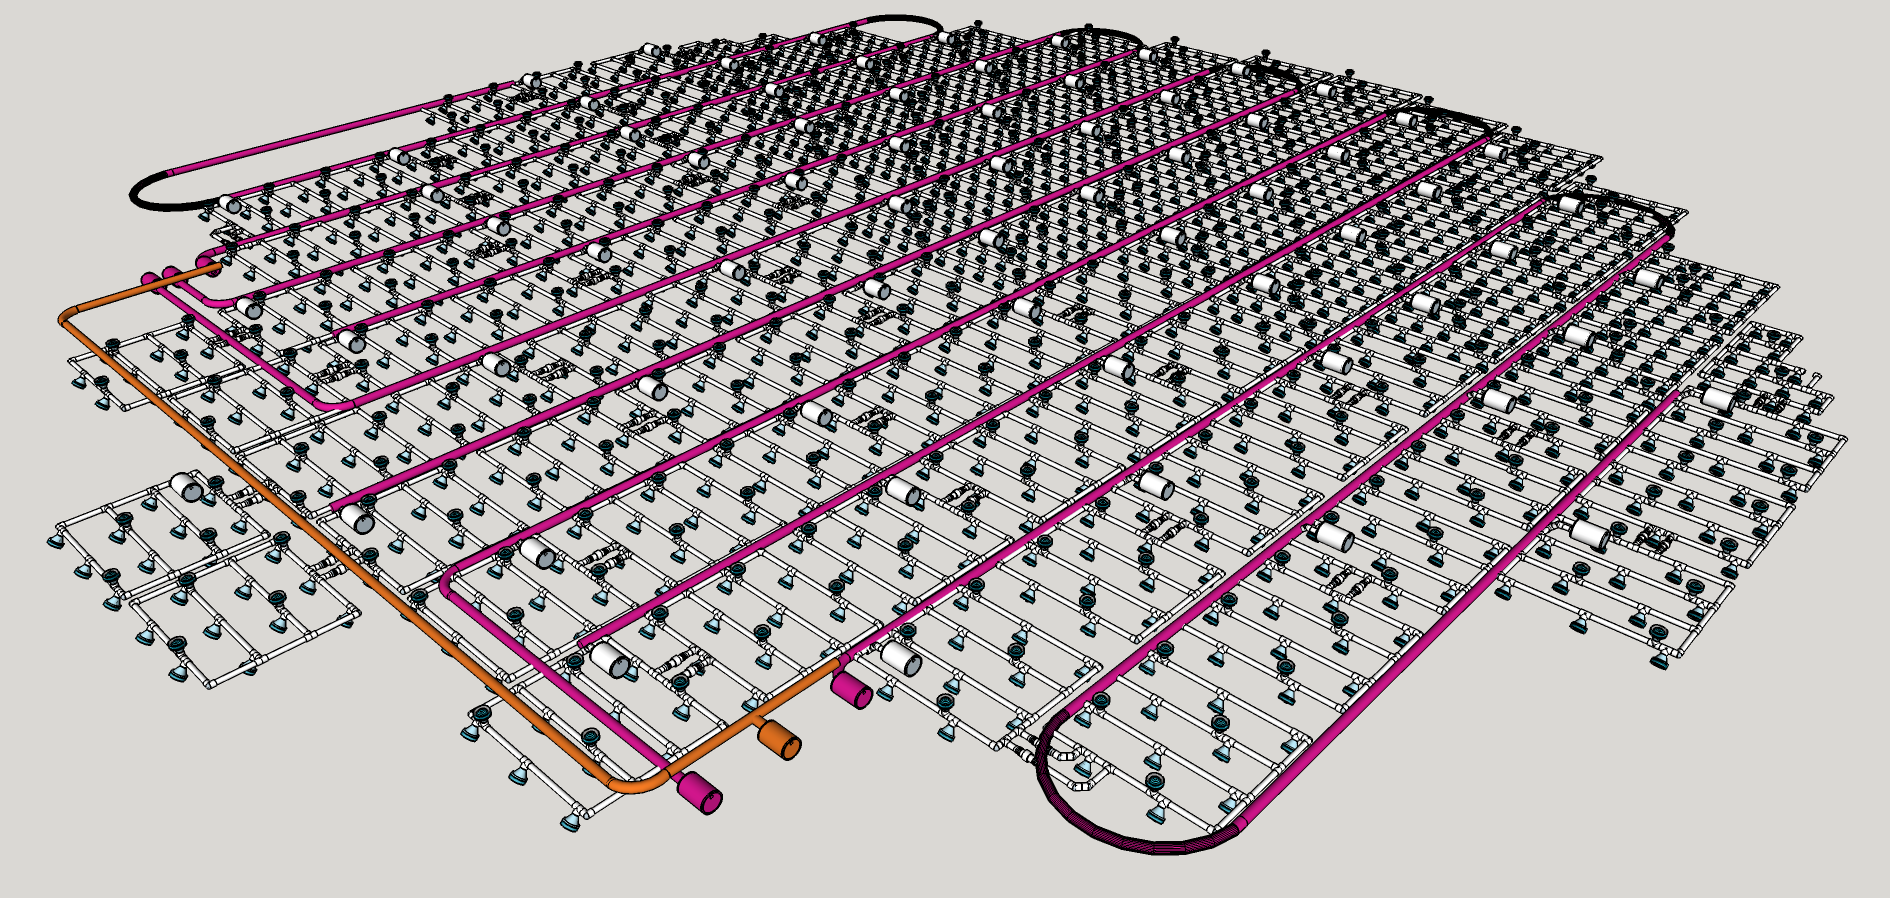
\includegraphics[width=\textwidth]{diagrams/4-chips/top_cap.png}
    \caption[Graphical rendering of the top-cap POMs.]
    {Graphical rendering of the top-cap POMs. Both the different photocathode coverage regions and
        the veto PMTs are visible.}
    \label{fig:top_cap}
\end{figure}

\subsection{Filtration} %%%%%%%%%%%%%%%%%%%%%%%%%%%%%%%%%%%%%%%%%%%%%%%%%%%%%%%%%%%%%%%%%%%%%%%%%%
\label{sec:chips_detector_water} %%%%%%%%%%%%%%%%%%%%%%%%%%%%%%%%%%%%%%%%%%%%%%%%%%%%%%%%%%%%%%%%%

Though surprisingly clear the Wentworth 2W pit water still requires filtration to reach the
required $\sim$\unit{30}{\mathrm{m}} attenuation length of light.

- Though remarkably clear the Wentworth pit water is not clean enough for the detector volume
where we require ~30m attenuation length. Need to pump water, to prevent algae blooms and
bacterial growth and remove particulates which are present in the water to begin with. An
umbilical resting on the pit floor will contain 2 fibres, 2 power cables and 2 flexible pipes for
filtering the internal water on shore. All connected to two shore huts, one for filtering and one
for data acquisition.

- A small positive pressure is kept inside the detector to prevent particulates coming in via and
leaks etc...

\subsection{Construction and deployment} %%%%%%%%%%%%%%%%%%%%%%%%%%%%%%%%%%%%%%%%%%%%%%%%%%%%%%%%%
\label{sec:chips_detector_deployment} %%%%%%%%%%%%%%%%%%%%%%%%%%%%%%%%%%%%%%%%%%%%%%%%%%%%%%%%%%%%

- How it can grow if needed - buoyant top cap anchored to the bottom one, which when fully
deployed will rest on the bottom of the pit.

\subsection{Current status} %%%%%%%%%%%%%%%%%%%%%%%%%%%%%%%%%%%%%%%%%%%%%%%%%%%%%%%%%%%%%%%%%%%%%%
\label{sec:chips_detector_status} %%%%%%%%%%%%%%%%%%%%%%%%%%%%%%%%%%%%%%%%%%%%%%%%%%%%%%%%%%%%%%%%

- No liner between veto and main volume!
- In the summer of 2018 and 2019 work on deploying \chips proceeded. Unforeseen hehe!!

This highlights one of the clear advantages of the \chips concept. No physical structure is
required on the barrel of the detector. Alongside the easier deployment discussed in
Section~\ref{sec:chips_detector_deployment} and the significantly simplified engineering, this is
the key reason as to why the \chips concept uses cylindrical rather than spherical detector
modules.

\begin{figure} % WORK DIAGRAM %
    \centering
    \subcaptionbox{gwgw}{%
        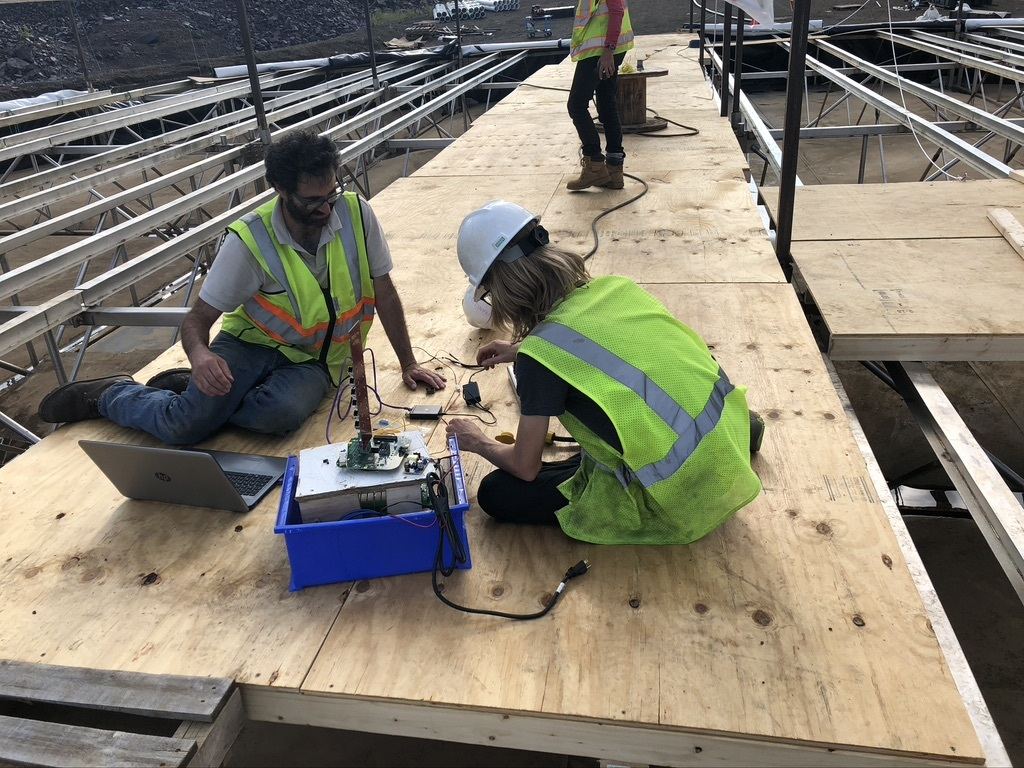
\includegraphics[height=5.5cm]{diagrams/4-chips/work1.jpeg}%
    }
    \quad
    \subcaptionbox{asgag}{%
        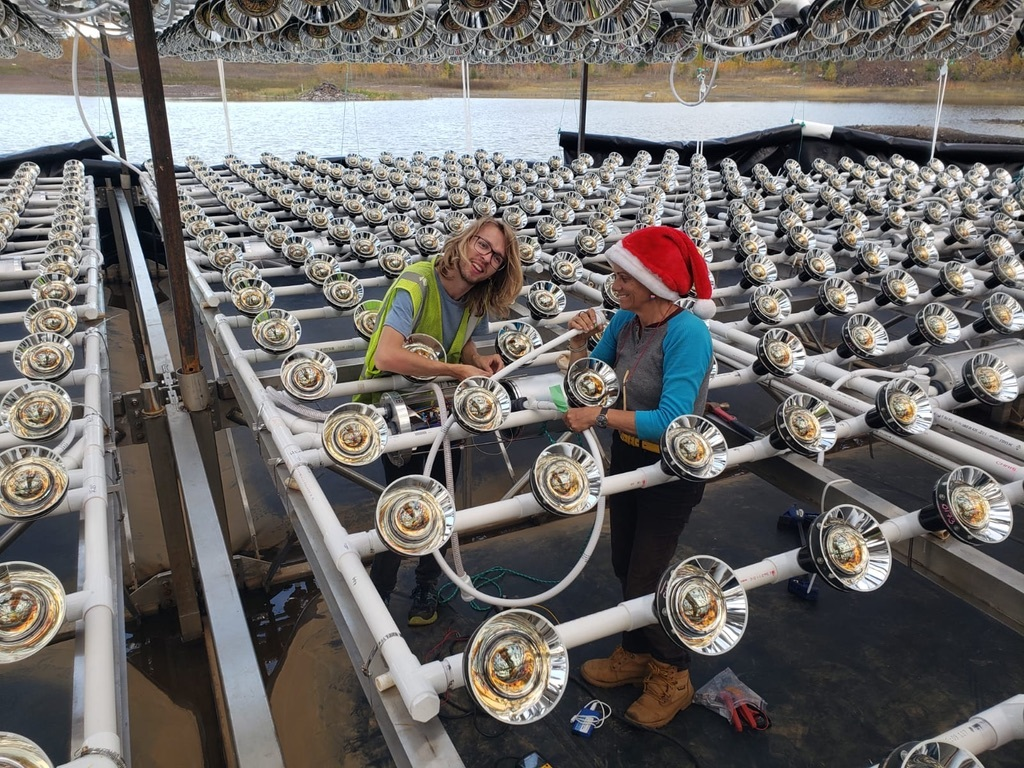
\includegraphics[height=5.5cm]{diagrams/4-chips/work2.jpeg}%
    }
    \caption[afaga]
    {afag}
    \label{fig:work}
\end{figure}

\begin{figure} % PANORAMA DIAGRAM %
    \includegraphics[width=\textwidth]{diagrams/4-chips/pan_1.jpeg}
    \caption[Panorama of the inside of \chipsfive just before deployment.]
    {Panorama of the inside of \chipsfive just before deployment. The six deployed Madison POMs
        are visible in the foreground on the bottom endcap. Additionally, the flexible tube manifolds
        can be seen connecting each POM to the higher level DAQ electronics.}
    \label{fig:pan_1}
\end{figure}

\section{Monte Carlo event generation and simulation} %%%%%%%%%%%%%%%%%%%%%%%%%%%%%%%%%%%%%%%%%%%%
\label{sec:chips_monte_carlo} %%%%%%%%%%%%%%%%%%%%%%%%%%%%%%%%%%%%%%%%%%%%%%%%%%%%%%%%%%%%%%%%%%%%

- Indispensable tool in particle physics, during the design and data analysis stages. Allows for
optimisation studies, testing of event reconstruction techniques and the study of potential
physics sensitivity.
- Useful MC simulation will provide output matching observables in a real detector. For full
analysis simulations need to be validated fully to make sure they approximate reality well enough.

\subsection{Beam event generation} %%%%%%%%%%%%%%%%%%%%%%%%%%%%%%%%%%%%%%%%%%%%%%%%%%%%%%%%%%%%%%%
\label{sec:chips_monte_carlo_beam} %%%%%%%%%%%%%%%%%%%%%%%%%%%%%%%%%%%%%%%%%%%%%%%%%%%%%%%%%%%%%%%

The expected energy spectrum (flux) of neutrinos at the \chipsfive detector location is generated
using the existing beam simulation written for the \numi beam experiments, and shown in
Fig.~\ref{fig:flux}. As the $\nu_{\tau}$ component is negligible, it is not predicted by the beam
simulation and ignored. Using the generated fluxes as input the GENIE neutrino event generator
(version 3.0.6)~\cite{andreopoulos2009, andreopoulos2015} is used to generate beam neutrino
events. Default cross-sections on water provided by GENIE are used. All initial, intermediate, and
final state particle tracks for each event are stored as output in a NUANCE formatted file for use
in the detector simulation. Note that unoscillated fluxes are used such that analyses samples must
be weighted to match the desired oscillated neutrino composition.

\begin{figure} % CHIPS FLUX DIAGRAM %
    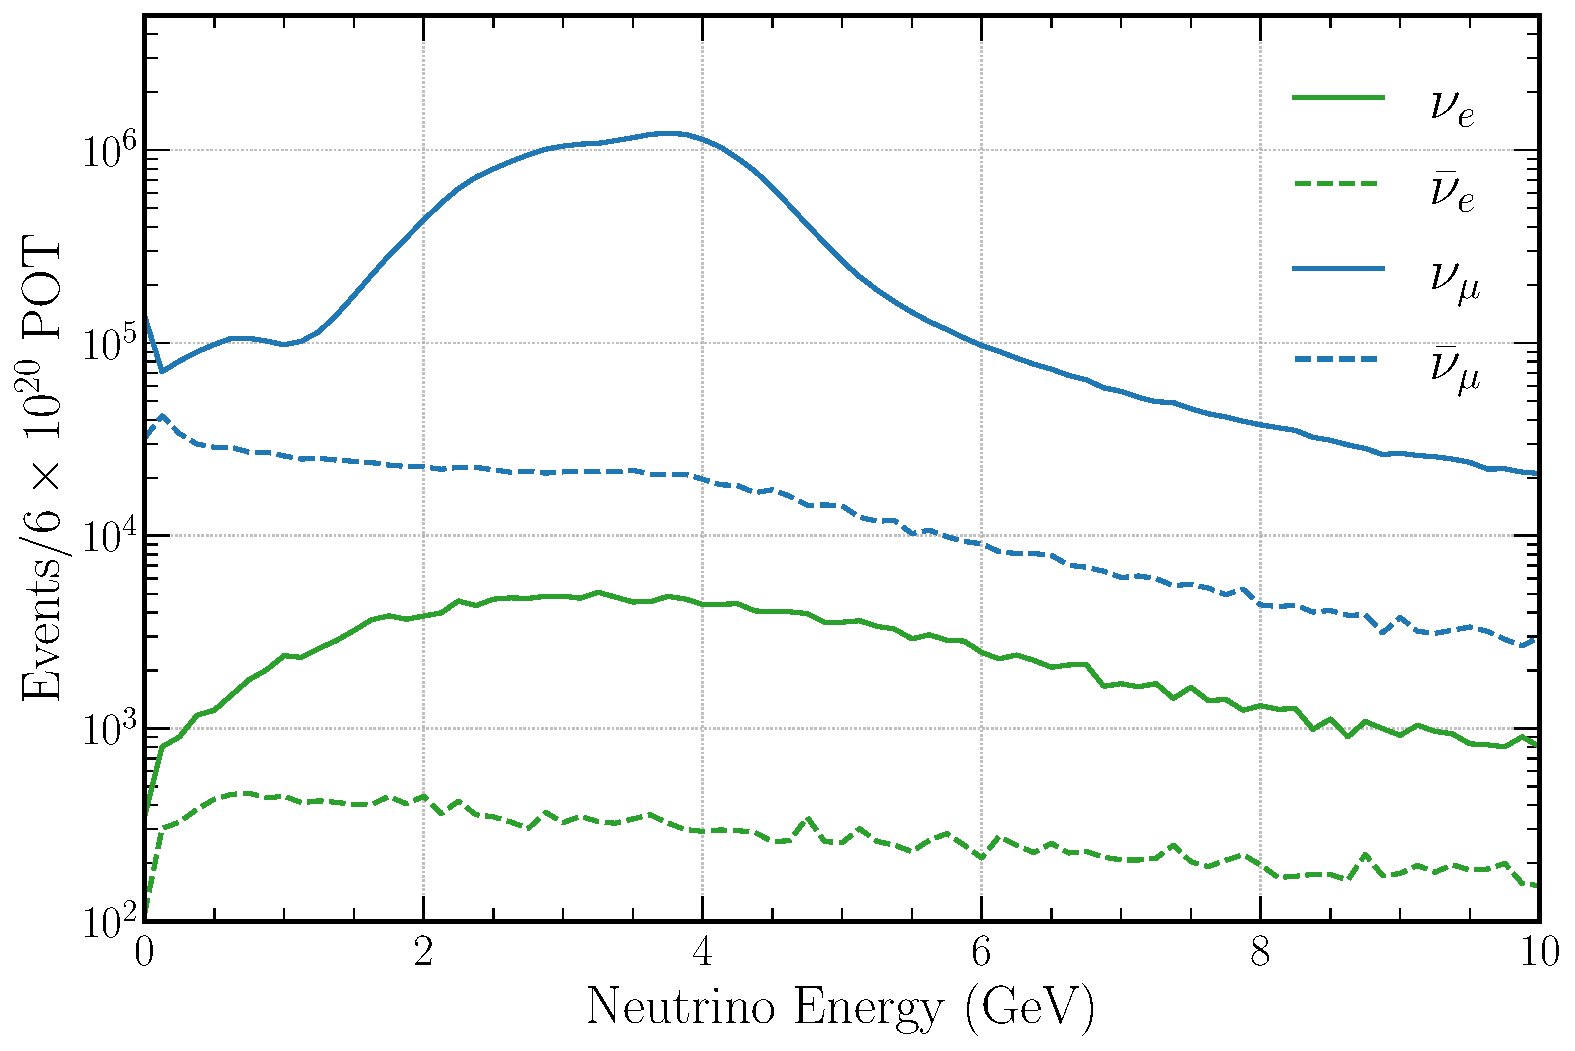
\includegraphics[width=0.8\textwidth]{diagrams/4-chips/flux.pdf}
    \caption[\numi neutrino flux at CHIPS.]
    {The neutrino mode (forward horn current) \numi beam neutrino energy spectrum at the
        \chipsfive detector module location. Shown are the separate contributions from the
        different neutrino types and signs. No cross-sections or oscillations have been applied.}
    \label{fig:flux}
\end{figure}

\subsection{Cosmic event generation} %%%%%%%%%%%%%%%%%%%%%%%%%%%%%%%%%%%%%%%%%%%%%%%%%%%%%%%%%%%%%
\label{sec:chips_monte_carlo_cosmic} %%%%%%%%%%%%%%%%%%%%%%%%%%%%%%%%%%%%%%%%%%%%%%%%%%%%%%%%%%%%%

The Cosmic-Ray Shower Library (CRY)~\cite{hagmann2012_1, hagmann2012_2} is used for cosmic ray
event generation. Both the solar cycle and Earth's geomagnetic field are taken into account, with
the \chipsfive latitude and deployment date (1st November 2019) used as input. Single muons are
generated at \emph{sea level} by CRY within a
\unit{1000}{\mathrm{m}}$\times$\unit{1000}{\mathrm{m}} area, with the detector at the centre.

Assuming a \chipsfive overburden of \unit{50}{\mathrm{m}} and a \unit{2.2}{\MeV/\mathrm{cm}^{2}}
muon energy loss in water as suggested in Ref.~\cite{klimushin2001} the muon parameters are
updated to estimate their values \unit{1}{\mathrm{m}} above the top of the detector. All muons
whose path does not cross the detector volume or do not have sufficient energy are discarded. All
accepted muon tracks are stored as output in a NUANCE formatted file for use in the detector
simulation~\cite{chipsgen2020}.

Extensive studies have looked at the likely cosmic rate for \chips detector modules at different
water overburden depths~\cite{son2013}. In this work, the fits shown in Fig.~\ref{fig:cosmic_rate}
for a cylindrical detector of both height and diameter \unit{24}{\mathrm{m}} are used to estimate
a cosmic muon rate of \unit{11.8}{\mathrm{KHz}} at \unit{50}{\mathrm{m}} of overburden for
\chipsfive. For the \unit{10}{\mu\mathrm{s}} long \numi beam spill occurring every
\unit{1.33}{\mathrm{s}} this gives an in spill cosmic rate of $\sim2.1$ million events per year
and an in spill occupancy of 9\%. Considering a typical event takes $\sim100\mathrm{ns}$ to
unfold, there is approximately a 0.3\% chance that any beam event overlaps with a cosmic muon.
This low coincidence shows just how powerful using a short beam spill is at reducing the cosmic
background.

\begin{figure} % COSMIC RATE DIAGRAM %
    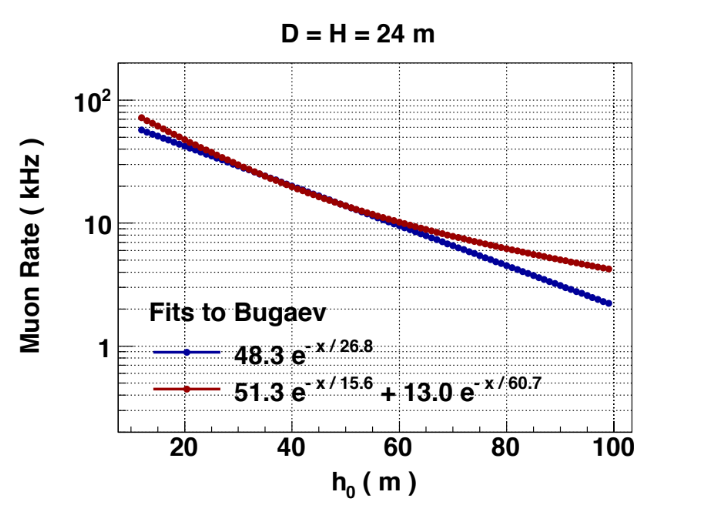
\includegraphics[width=0.6\textwidth]{diagrams/4-chips/cosmic_rate.png}
    \caption[Expected \chipsfive cosmic muon rate as a function of depth.]
    {Expected cosmic muon rate as a function of water overburden depth for a \unit{24}{\mathrm{m}}
        high and \unit{24}{\mathrm{m}} wide \chips detector module. Shown are fits made to the work
        originally conducted in Ref.~\cite{bugaev1998}. Figure taken from Ref.~\cite{son2013}.}
    \label{fig:cosmic_rate}
\end{figure}

\subsection{Detector simulation} %%%%%%%%%%%%%%%%%%%%%%%%%%%%%%%%%%%%%%%%%%%%%%%%%%%%%%%%%%%%%%%%%
\label{sec:chips_monte_carlo_sim} %%%%%%%%%%%%%%%%%%%%%%%%%%%%%%%%%%%%%%%%%%%%%%%%%%%%%%%%%%%%%%%%

The detector simulation uses the WCSim water Cherenkov simulation package~\cite{wcsim2020} built
on top of the Geant4 simulation framework~\cite{agostinelli2003, allison2006, Allison2016}.
Originally developed to simulate possible water Cherenkov detectors in the LBNE beam (now LBNF),
WCSim is now used more widely in the field for generic water Cherenkov detectors. WCSim has been
heavily modified for the \chips project to allow for generic water Cherenkov detector geometries
to be easily loaded at runtime via a series of simple XML configuration files. These changes allow
for a broad range of detector geometries to be quickly considered without recompilation of the
code.

To represent \chips detector modules, the simulation builds an n-sided, regular polygonal prism
consisting of two endcaps separated by a barrel. The prism is filled with water and lined with a
low reflectivity \emph{blacksheet}. The geometry is separated into \emph{regions} within both the
barrel and endcaps, defined either by a list of barrel sides or an opening angle respectively.
Each region is filled with a unique base unit of geometry known as the \emph{unit cell} as shown
in Fig.~\ref{fig:sim_geom}.

The unit cell defines a pattern of any number of PMTs, as well as their relative positions and in
which direction they face. The final geometry is built by tiling each of the defined regions with
their respective unit cell scaled to match the required regional photocathode coverage. Note that
although exact PMT positions are not used in this procedure, a given configuration always
generates the same geometry (it is deterministic). In this work the \chipsfive geometry is
generated with 28 sides regions matching the angles and photocathode coverage outlined in
Section.~\ref{sec:chips_detector_instrumentation}.

\begin{figure} % SIMULATION GEOM DIAGRAM %
    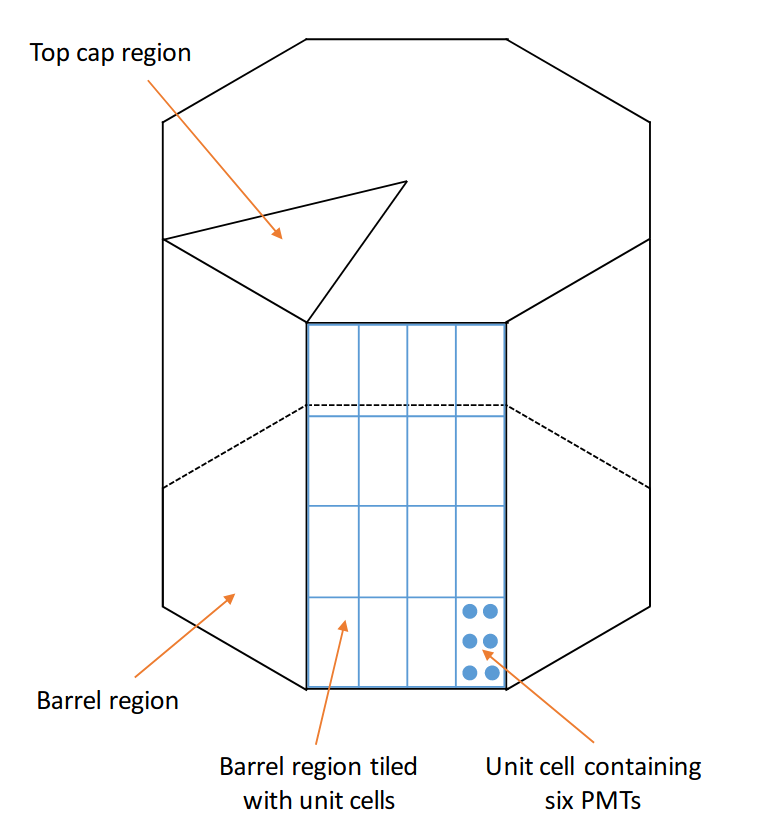
\includegraphics[width=0.6\textwidth]{diagrams/4-chips/sim_geom.png}
    \caption[Illustrative diagram of a WCSim detector geometry.]
    {Illustrative diagram of a WCSim detector geometry, showing the shape, endcap and barrel
        regions, tiled unit cells and PMTs within a unit cell. Figure taken from
        Ref.~\cite{blake2016}.}
    \label{fig:sim_geom}
\end{figure}

The geometry shape, regions, and unit cells are defined in a configuration file. Additionally, a
file for PMT definitions containing their shape, time resolution, and quantum efficiency is
defined. Light cones are described by a list of radial profile points in a further file. Although
the underlying Geant4 material properties are mostly hardcoded (taken from the Super-Kamiokande
simulation) they can be scaled by values within yet another configuration file. This file controls
the water absorption and scattering (Rayleigh and Mie) lengths, and both the blacksheet and PMT
glass reflectivity. In this work an attenuation length of \unit{50}{\mathrm{m}} at
\unit{405}{\mathrm{nm}} is used with negligible scattering, the blacksheet reflectivity is set to
be 4\% and the PMT glass reflectivity 24\%.

A veto volume can also be defined. The veto is built as either a concentric shell around the whole
inner volume with a given thickness or solely above the top-cap with a given height. Any PMTs
defined as facing outwards within a unit cell look into the veto volume instead of the inner
volume.

Once the full generation of the runtime Geant4 geometry is complete, the final state tracks for
each successive event to be simulated are loaded from either the beam or cosmic event generator
NUANCE files. Beam event vertices are randomly placed within the inner detector volume, while
cosmic vertices are kept at \unit{1}{\mathrm{m}} above the detector volume. WCSim then simulates
the passage of all particles through the detector materials, with interactions, decays, and
Cherenkov emission also considered.

Whenever a photon is calculated to have hit the photocathode of a PMT an angular dependent
acceptance efficiency is applied to see if it it is recorded. If accepted all hits within
\unit{200}{\mathrm{ns}} windows are grouped together to output a single `recorded' PMT hit, with
the smeared first photon hit time used as the recorded hit time. 

Whenever a photon is calculated to have hit the photocathode of a PMT a digitisation simulation is
used to convert the true photon hits into a `recorded' charge in photoelectrons. All hits within
\unit{200}{\mathrm{ns}} windows are grouped together for each recorded hit, with the first smeared
photon hit time used. A method similar the that used in the Super-Kamiokande simulation is used to
calculate the overall charge. For each photon a single photoelectron charge distribution is probed
and the combined sum returned. By sampling this procedure many times the probability distribution
given a number of input photons is given in Fig.~\ref{fig:digitisation}.

\begin{figure} % DIGI DIAGRAM %
    \centering
    \subcaptionbox{\label{fig:digi_method}}{%
        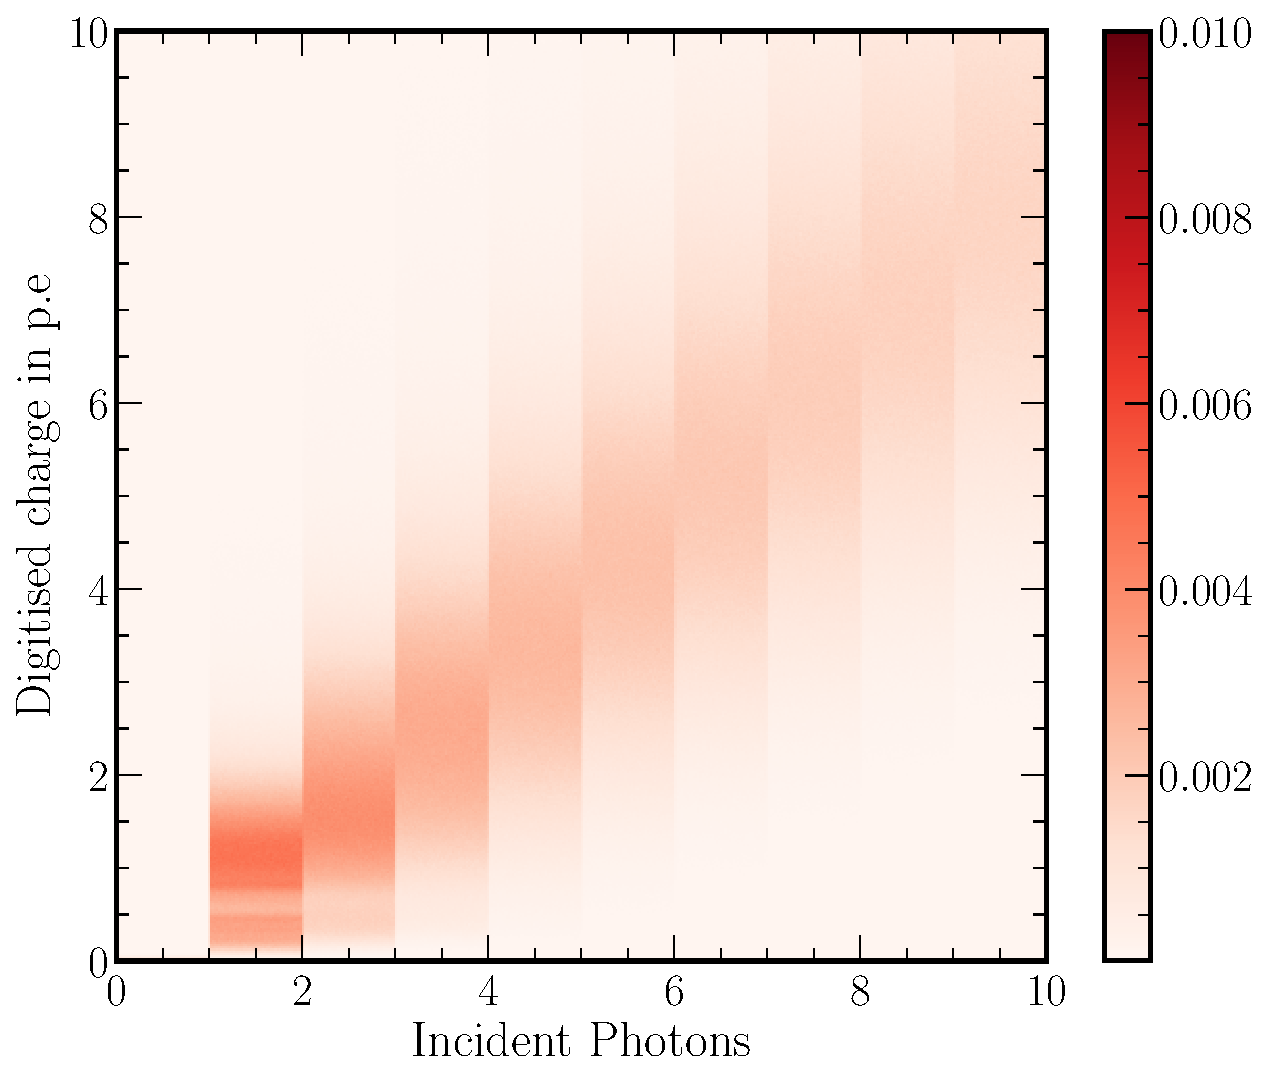
\includegraphics[height=6cm]{diagrams/4-chips/digi_method.pdf}%
    }
    \quad
    \subcaptionbox{\label{fig:digi_likelihood}}{%
        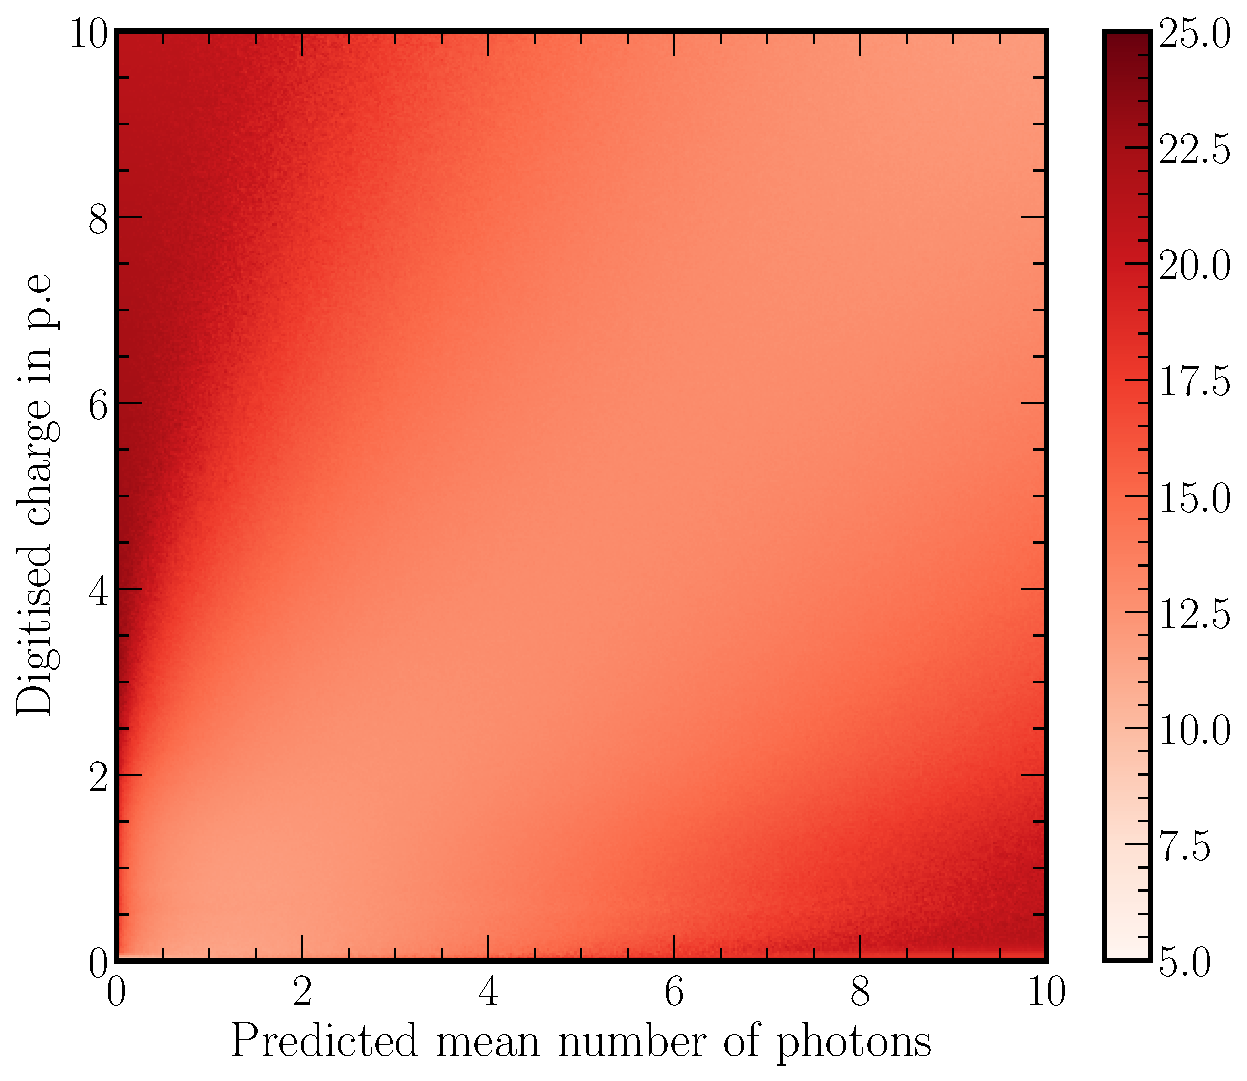
\includegraphics[height=6cm]{diagrams/4-chips/digi_likelihood.pdf}%
    }
    \caption[Detector simulation PMT digitisation function.]
    {The detector simulation digitisation probability function (a) used for the Nikhef

        (a) Digitisation probability function used within the simulation to convert incident photons
        to a measured digitised charge. (b) Likelihood of a measured digitised charge being caused
        by a number of photons incident on a PMT.}
    \label{fig:digitisation}
\end{figure}

- Angular efficiency
- default Geant4 physics list is used (QGSP\_BIC\_HP).
- The digitisation function could definitely be improved.
- All hits are recorded as output!!!

\begin{figure} % SIMULATED EVENT DISPLAY DIAGRAM %
    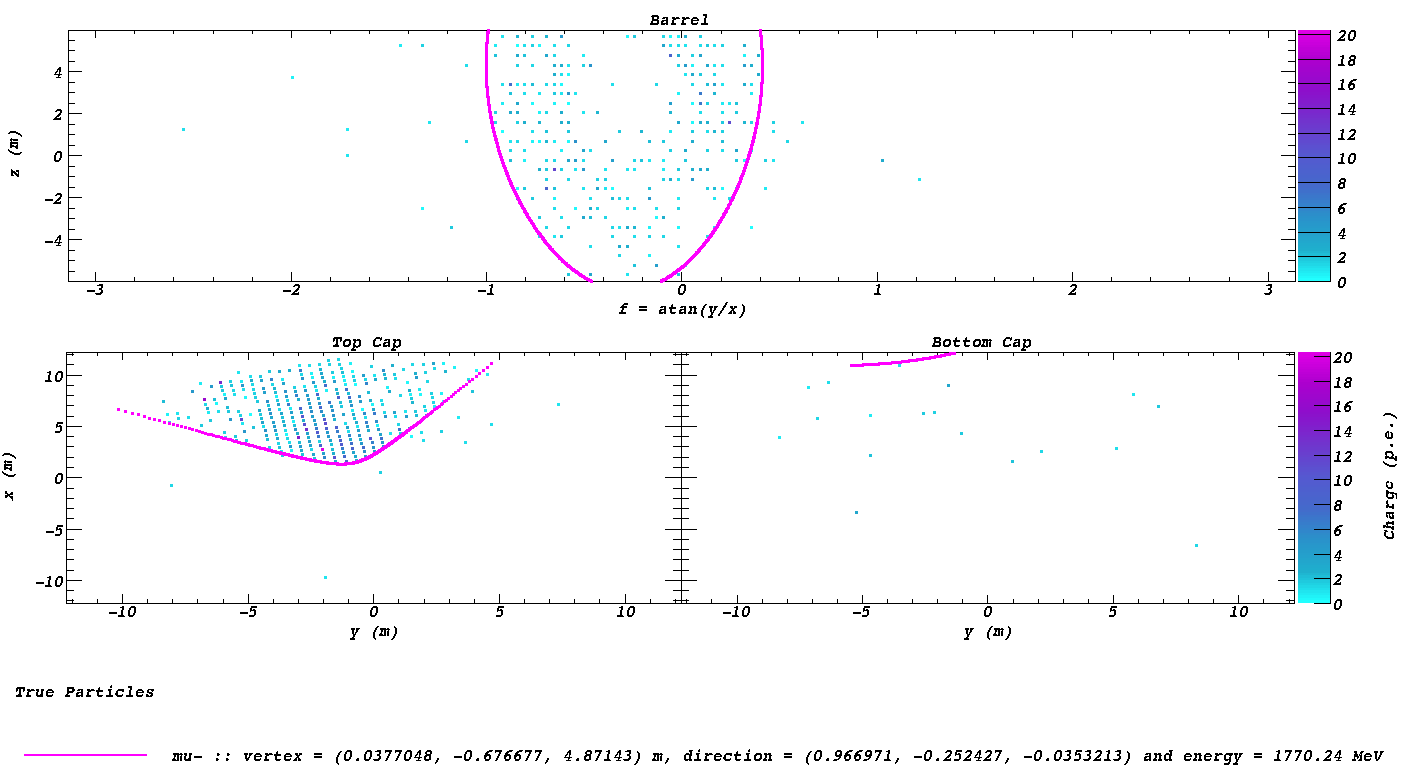
\includegraphics[width=\textwidth]{diagrams/4-chips/sim_event.png}
    \caption[sim event short]
    {Event display of a simulated CC $\nu_{\mu}$ quasi-elastic event with a single muon in the
        final state of energy \unit{1.77}{\GeV}. The display shows both the unrolled barrel of the
        \chipsfive detector as well the two endcaps. Every coloured entry represents a hit PMT
        with the color indicating the total photoelectrons (charge) collected. The pink ring is a
        projection of the true Cherenkov light cone associated with the muon track from the
        interaction vertex.}
    \label{fig:sim_event}
\end{figure}

%%%%%%%%%%%%%%%%%%%%%%%%%%
- These short spills are essential for \chips and other experiments in rejecting the massive
cosmic ray background. As all events outside the expected beam spill window at the detector can be
rejected.
- Only single cosmic muons are considered for simplicity, future work should also consider
electrons, pions and multiple cosmic muons at the same time.

    \chapter{Data acquisition for CHIPS} %%%%%%%%%%%%%%%%%%%%%%%%%%%%%%%%%%%%%%%%%%%%%%%%%%%%%%%%%%%%%
\label{chap:daq} %%%%%%%%%%%%%%%%%%%%%%%%%%%%%%%%%%%%%%%%%%%%%%%%%%%%%%%%%%%%%%%%%%%%%%%%%%%%%%%%%

The primary task of any Data Acquisition system is the processing of low-level signals measuring
real-world physics and their transfer to permanent storage for further analysis. Commonly, this
procedure also includes decision making as to whether the signal is deemed interesting enough to
record, known as a \emph{trigger}. Both these tasks can make DAQ systems incredibly complex,
especially when they must operate in an efficient and resilient manner for vast amounts of data in
real-time, while also providing detector control and monitoring.

In the context of the \chips project, the DAQ system records all PMT hits, timestamps them using a
common clock, and transfers them out of the detector to a central processing node. This node then
applies a trigger to select hits that fall within the interesting \numi beam spill time window,
before the selected hits are sliced into events and moved to permanent storage for further
analysis. Alongside these processes, the DAQ system also configures the detector and provides data
quality and detector component monitoring.

Although relatively simple when compared to the incredibly complex and time-pressured DAQ systems
of the LHC experiments, the DAQ system developed for the \chips project introduces some novel
approaches to solve the unique constraints of the \chips concept. Namely, deployment within a body
of water and a limited resource budget. In this chapter, the DAQ system for \chips as applied to
the \chipsfive prototype detector module is described alongside highlighting any novel approaches.
The description is presented in two broad categories, hardware and software, with a short
description of the timing system beforehand.

\section{White Rabbit timing} %%%%%%%%%%%%%%%%%%%%%%%%%%%%%%%%%%%%%%%%%%%%%%%%%%%%%%%%%%%%%%%%%%%%
\label{sec:daq_timing} %%%%%%%%%%%%%%%%%%%%%%%%%%%%%%%%%%%%%%%%%%%%%%%%%%%%%%%%%%%%%%%%%%%%%%%%%%%

To ensure PMT hit times are synchronised throughout \chips detectors, a common clock must be
shared across all timestamping electronics. For this purpose, \chips uses a \emph{White Rabbit}
(WR) network~\cite{lipinski2011}. Initially developed at CERN, the open-source WR project provides
an ethernet-based time distribution network with sub-nanosecond synchronisation accuracy between
nodes. By using two-way exchanges of WR messages, precise adjustment of individual node clock
phases and offsets is possible across thousands of devices, separated by tens of kilometres. All
of this is achieved in parallel with a standard data transfer network capable of
\unit{1}{\text{Gb}} speeds.

All nodes are synchronised to the clock of a \emph{GrandMaster} node, typically a WR
\emph{switch}, the most common WR hardware component. As input, the switch receives an IRIG-B
(Inter-Range Instrumentation Group timecode B) and a \unit{10}{\text{MHz}} signal from a GPS
disciplined oscillator. These inputs allow for synchronisation of the GrandMaster clock to
International Atomic Time (TAI). As \chips detector modules require synchronisation to accelerator
clocks many hundreds of kilometres away to determine the arrival time of beam spills, the GPS
disciplined timing is particularly important.

WR hardware is commercially available from many vendors. Within \chipsfive, two WR devices are
used for time synchronisation and data transfer, both shown in Fig.~\ref{fig:wr_electronics}.
Firstly, a compact version of the standard WR switch~\cite{wrswitch2020}, specially developed for
the \chips project at Nikhef~\cite{wrchromium2020}. Secondly, a WR-LEN (Lite Embedded Node) from
Seven Solutions~\cite{wrlen2020}. 

\begin{figure} % WHITE-RABBIT COMPONENTS DIAGRAM %
    \centering
    \subcaptionbox{White Rabbit switch}{%
        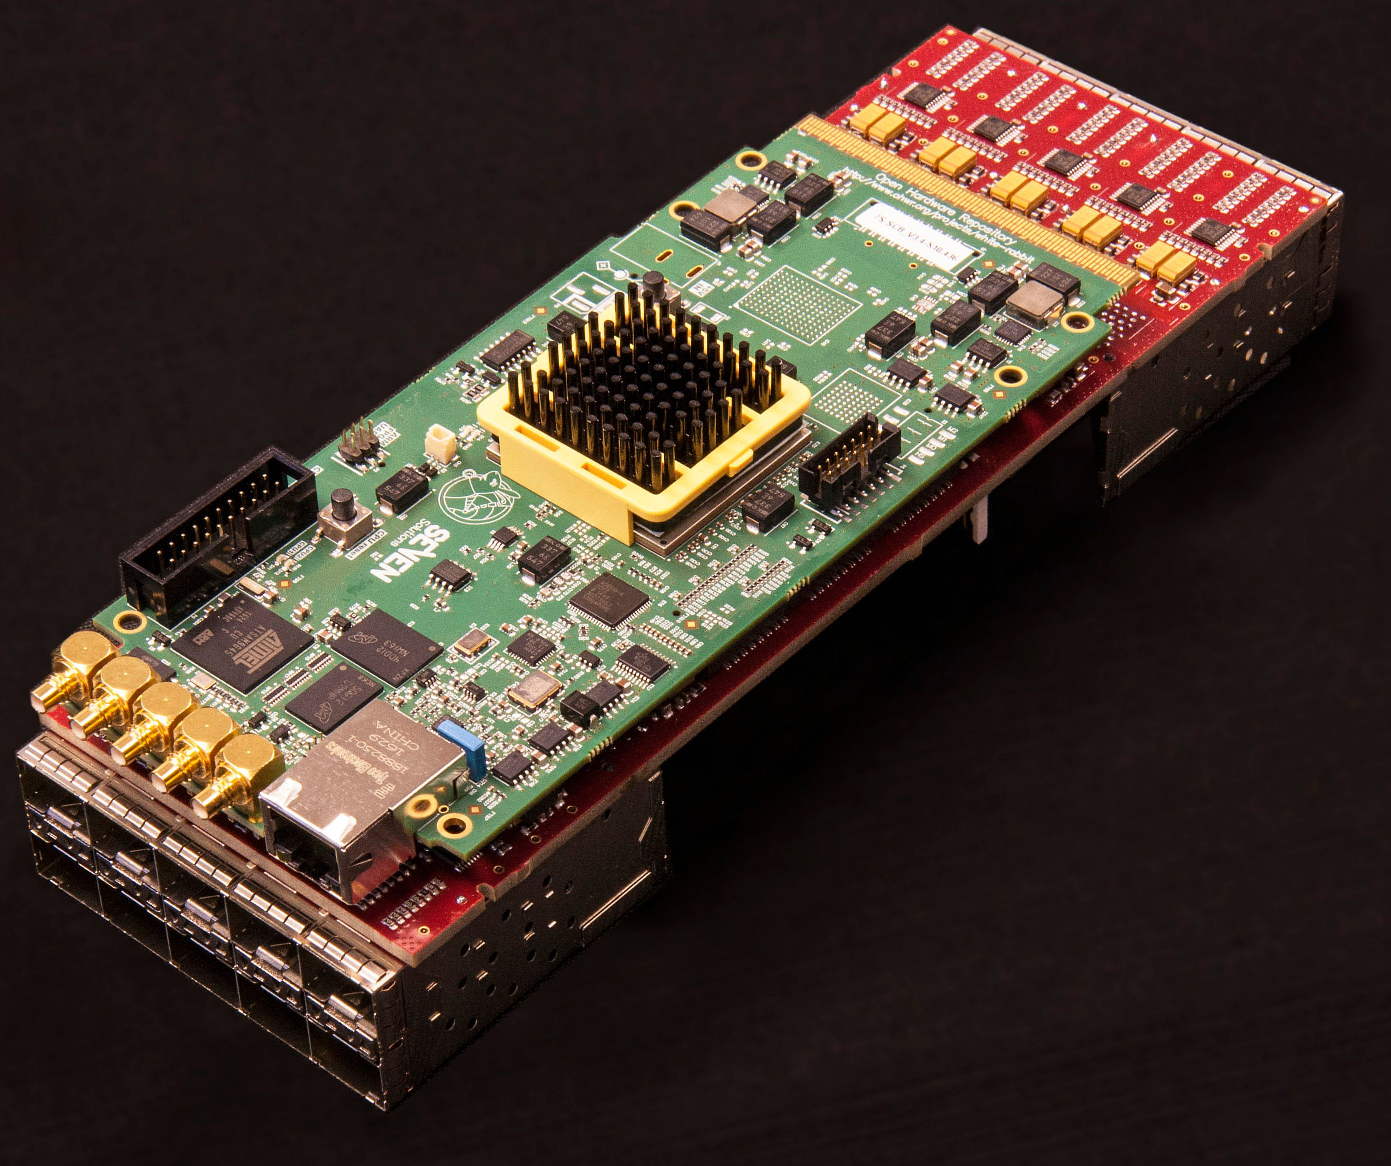
\includegraphics[height=6cm]{diagrams/5-daq/wr_switch.pdf}%
    }
    \quad
    \subcaptionbox{White Rabbit LEN}{%
        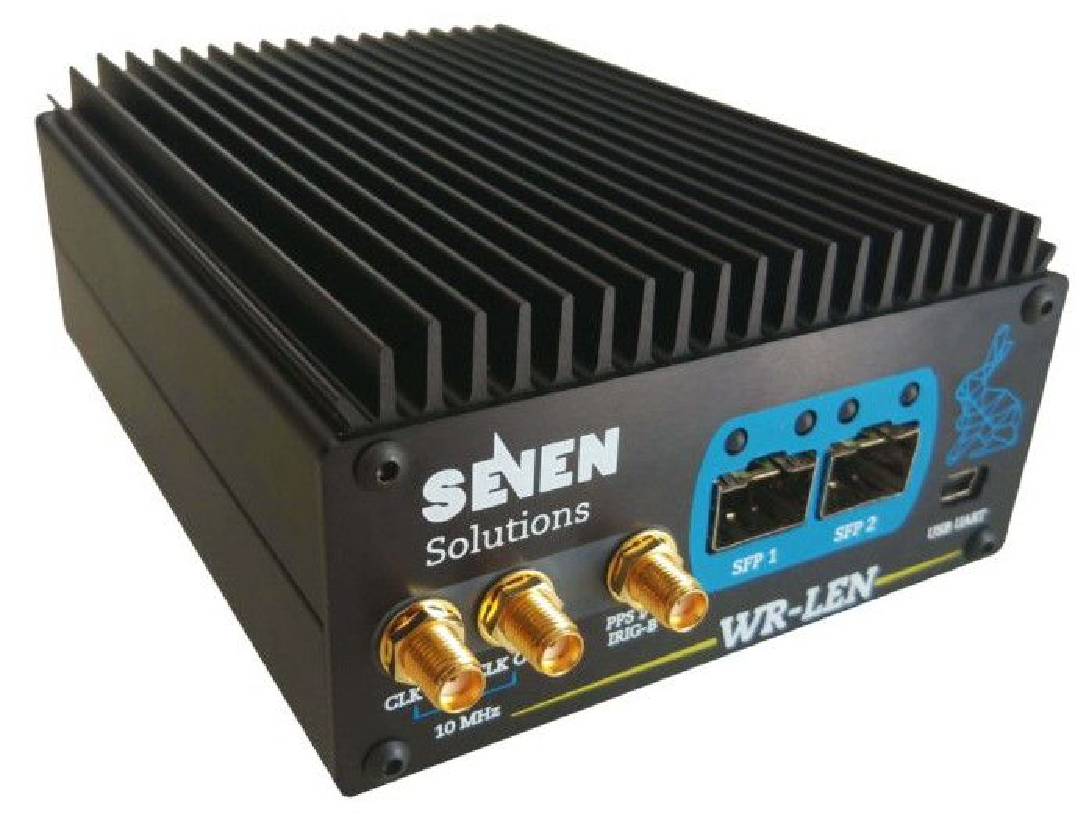
\includegraphics[height=6cm]{diagrams/5-daq/wr_len.pdf}%
    }
    \caption[Pictures of the White Rabbit timing hardware used within \chipsfive]
    {Pictures of the White Rabbit timing hardware used within \chipsfive. The compact White rabbit
        switch  specially designed for \chips is shown in (a), while the White Rabbit Lite
        Embedded Node (WR-LEN) from Seven Solutions is shown in (b).}
    \label{fig:wr_electronics}
\end{figure}

All WR components are connected using \unit{1}{\text{Gb}} bi-directional optical fibre
connections, using the \unit{1310}{\text{nm}} and \unit{1550}{\text{nm}} wavelengths via Small
Form-Factor Pluggable Transceivers (SFPs). Fig.~\ref{fig:sync} shows the subsequent WR
synchronised pulse per second clock rising edges for two \chipsfive WR switches separated by
\unit{500}{\text{m}} of fibre. With the vertical ticks representing single nanoseconds,
sub-nanosecond time synchronisation accuracy between the switches is observed.

\begin{figure} % WHITE-RABBIT SYNC DIAGRAM %
    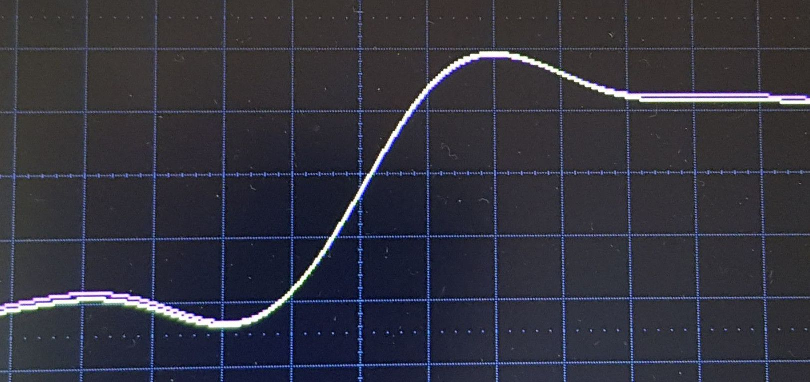
\includegraphics[width=0.7\textwidth]{diagrams/5-daq/sync.pdf}
    \caption[Picture of White Rabbit timing synchronisation seen within \chipsfive]
    {Picture of an oscilloscope display measuring the pulse per second output signal from two WR
        switches shown in pink and yellow at either end of a \unit{500}{\text{m}} long optical
        fibre. The vertical ticks are in nanoseconds showing the sub-nanosecond synchronisation
        possible with the WR timing network.}
    \label{fig:sync}
\end{figure}

\section{Hardware} %%%%%%%%%%%%%%%%%%%%%%%%%%%%%%%%%%%%%%%%%%%%%%%%%%%%%%%%%%%%%%%%%%%%%%%%%%%%%%%
\label{sec:daq_hard} %%%%%%%%%%%%%%%%%%%%%%%%%%%%%%%%%%%%%%%%%%%%%%%%%%%%%%%%%%%%%%%%%%%%%%%%%%%%%

The hardware of the \chipsfive DAQ system is split into two distinct implementations at its lower
levels (closest to the PMTs), corresponding to the Nikhef and Madison \textsc{Pom} types. \chips
R\&D efforts have principally developed the novel Madison implementation with the view to use this
hardware within detector modules exclusively. However, as a safe stepping stone, while development
and testing are still ongoing, \chipsfive mainly contains proven Nikhef hardware developed for the
KM3NeT experiment~\cite{adrian2016}.

The complete DAQ and power distribution system for \chipsfive is diagrammatically shown in
Fig.~\ref{fig:daq}. The following subsections describe each component, starting from the lowest
level and working upwards. The Nikhef and Madison descriptions are separated for clarity as well
as the high-level combined hardware systems, part of which is not physically located within the
detector but onshore in an electronics hut (separate from the water filtration hut).

\begin{figure} % DAQ DIAGRAM %
    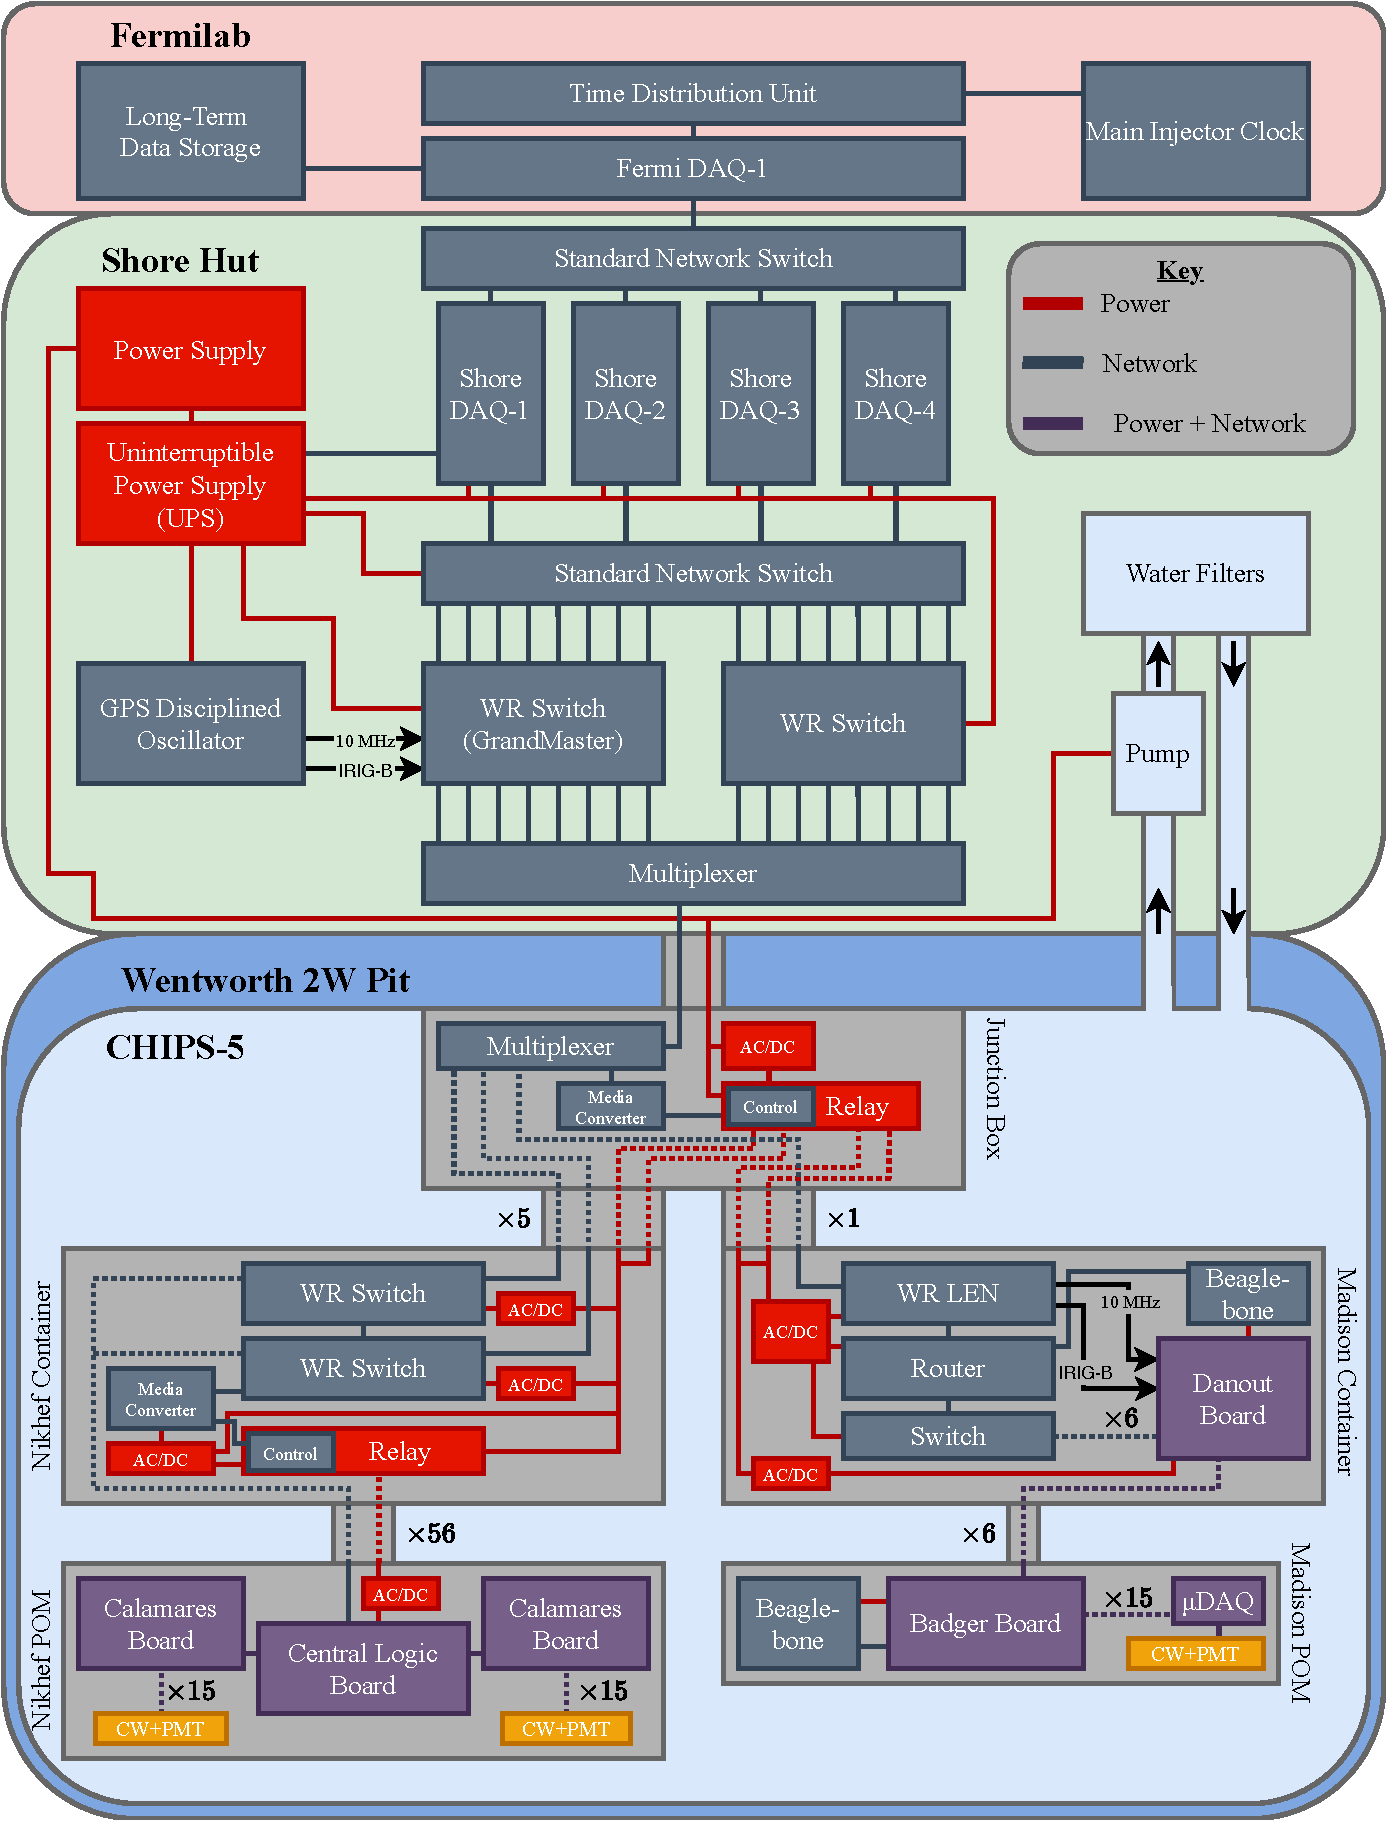
\includegraphics[width=\textwidth]{diagrams/5-daq/daq.pdf}
    \caption[Diagram of the complete \chipsfive data acquisition and power distribution system]
    {Diagram of the complete \chipsfive DAQ and power distribution system.}
    \label{fig:daq}
\end{figure}

Common to both low-level hardware implementations is the use of the Time over Threshold (ToT)
method for PMT signal digitisation. Each analogue PMT pulse is fed to a ToT discriminator coupled
with a Time to Digital Converter (TDC) to generate each digitised recorded hit, as shown in
Fig.~\ref{fig:tot}. Compared to the more common Analogue to Digital Converter (ADC) readout, ToT
values are less accurate and do not scale linearly with deposited charge. However, the ToT
methodology is used within \chips as the electronics is simpler and notably cheaper.

\begin{figure} % TOT DIAGRAM DIAGRAM %
    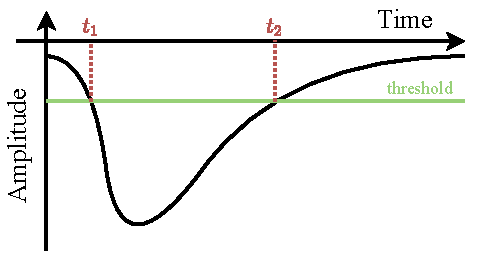
\includegraphics[width=0.6\textwidth]{diagrams/5-daq/tot.pdf}
    \caption[Illustrative diagram showing how Time over Threshold is measured]
    {Illustrative diagram showing how a ToT value is measured. As soon as the rising edge of a PMT
        charge pulse rises above a given threshold (goes below in the negative charge case) a time
        is recorded $t_{1}$, when the falling edge later falls below the threshold a second time
        $t_{2}$ is recorded. The difference in time between $t_{1}$ and $t_{2}$ is output by the
        electronics as a digitised ToT value.}
    \label{fig:tot}
\end{figure}

\subsection{Nikhef hardware} %%%%%%%%%%%%%%%%%%%%%%%%%%%%%%%%%%%%%%%%%%%%%%%%%%%%%%%%%%%%%%%%%%%%%
\label{sec:daq_hard_Nikhed} %%%%%%%%%%%%%%%%%%%%%%%%%%%%%%%%%%%%%%%%%%%%%%%%%%%%%%%%%%%%%%%%%%%%%%

All Nikhef HZC PMTs are attached directly to a simple readout board containing a high-voltage
generating Cockcroft-Walton circuit. Up to 30 such PMTs are connected to two \emph{Calamares}
boards within the electronics box of each Nikhef \textsc{Pom} via standard category 5 cables with
RJ45 connectors, as shown in Fig.~\ref{fig:nikhef_plane}. Both Calamares boards are directly
attached to a \emph{Central Logic Board} (CLB)~\cite{biagi2015, eijk2015}. The CLB contains ToT
discriminators and TDCs to digitise the recorded signals as well as electronics to synchronise to
the WR network clock for timestamping. Each Nikhef \textsc{Pom} electronics box also contains an
AC to DC power converter (AC/DC) whose output is fed into the CLB for power distribution.

\begin{figure} % NIKHEF PLANE DIAGRAM %
    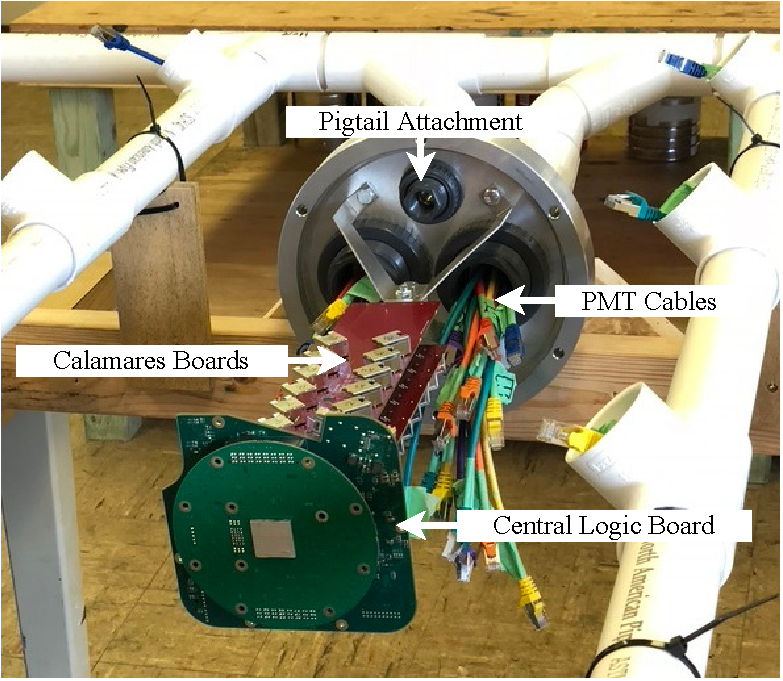
\includegraphics[width=0.8\textwidth]{diagrams/5-daq/nikhef_plane.pdf}
    \caption[Labelled picture of the Nikhef \textsc{Pom} electronics box]
    {Labelled picture of the Nikhef \textsc{Pom} electronics box without its aluminium casing.
        Both ends of the category 5 PMT cables can be seen, either at the PMT mounting points or
        entering the electronics box and not yet plugged into Calamares boards.}
    \label{fig:nikhef_plane}
\end{figure}

Every Nikhef \textsc{Pom} is connected via a single optical fibre and a single power connection to
a \emph{Nikhef-container}, the contents of which are labelled in the bottom half of
Fig.~\ref{fig:full_setup}. Two WR switches are used within each container to provide sufficient
\textsc{Pom} networking ports. Both switches are powered by independent AC to DC converters and
connected via a single optical fibre each to the higher level DAQ systems. An additional
connection between each switch ensures that if one higher-level connection fails the other can
still be used.

Each Nikhef-container also contains a relay board to control the power supply to individual
\textsc{Pom}s. The relay board control electronics are powered via an AC to DC converter and
connected to one of the switches via a media converter for networking. The media converter is
required to convert the optical fibre WR switch connection to a standard RJ45 copper cable
connection. A total of five Nikhef-containers are present within \chipsfive.

\begin{figure} % FULL SETUP DIAGRAM %
    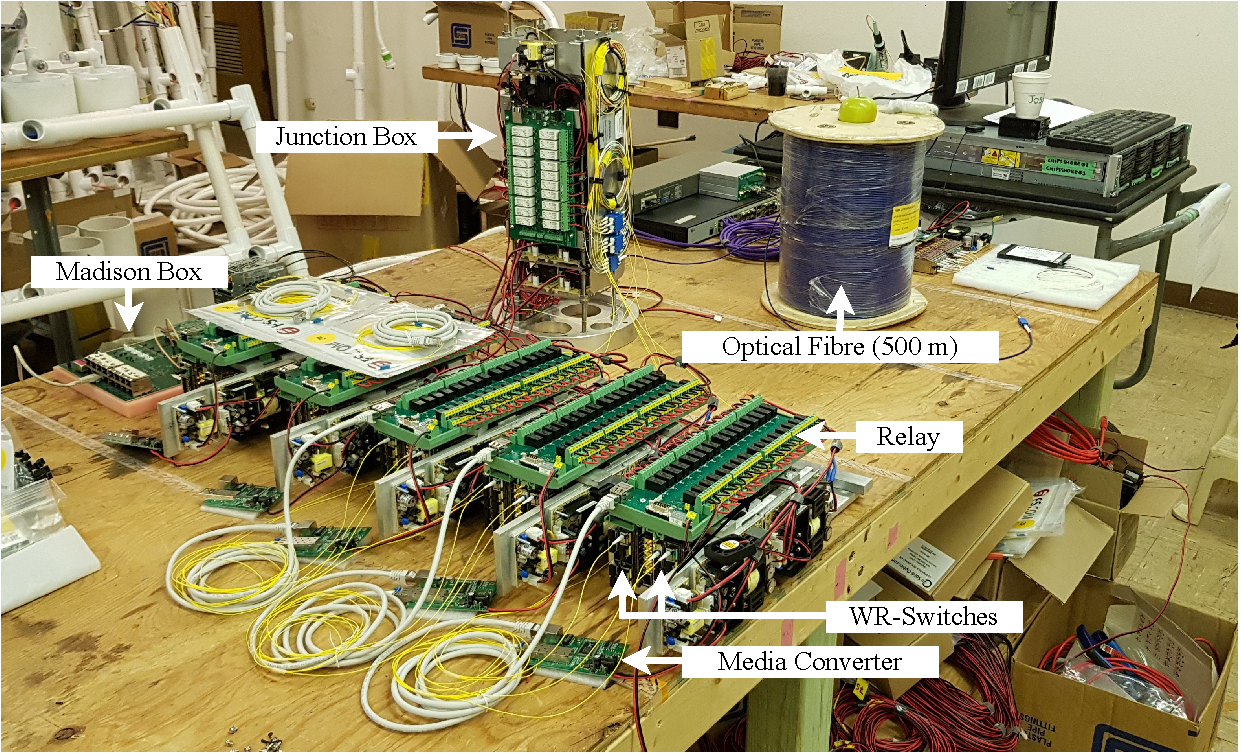
\includegraphics[width=\textwidth]{diagrams/5-daq/full_setup.pdf}
    \caption[Picture of the non \textsc{Pom} components of the \chipsfive DAQ system]
    {Picture of the non \textsc{Pom} components of the \chipsfive DAQ system arranged on a table
        at the PolyMet mining administration building.}
    \label{fig:full_setup}
\end{figure}

\subsection{Madison hardware} %%%%%%%%%%%%%%%%%%%%%%%%%%%%%%%%%%%%%%%%%%%%%%%%%%%%%%%%%%%%%%%%%%%%
\label{sec:daq_hard_madison} %%%%%%%%%%%%%%%%%%%%%%%%%%%%%%%%%%%%%%%%%%%%%%%%%%%%%%%%%%%%%%%%%%%%%

Every Madison Hamamatsu PMT is directly attached to a high-voltage generating Cockcroft-Walton
board followed by a signal processing $\micro$DAQ, as shown in
Fig.~\ref{fig:madison_pmt_assembly}. The $\micro$DAQ is a small microcontroller developed for both
IceCube and \chips at WIPAC in Madison. Capable of timestamping and digitising signals directly at
the PMT level, the $\micro$DAQ also sets the PMT operating voltage by controlling the driving
frequency of the Cockcroft-Walton board~\cite{eijk2018}.

Up to 16 $\micro$DAQs receive power, networking, and WR synchronised IRIG-B and
\unit{10}{\text{MHz}} timing signals from a \emph{badger-board}, as shown in
Fig.~\ref{fig:madison_plane}. Standard category 5 cables with RJ45 connectors are used for these
connections. The badger-board is located within the electronics box of each Madison \textsc{Pom}
and acts as a simple fanout and power control board. For logic, each badger-board has an attached
mezzanine Beaglebone~\cite{beagle2020}. This single-board Linux machine (very similar to a
Raspberry Pi) controls the power supply to, and receives hits from, the attached $\micro$DAQs.

\begin{figure} % MADISON PLANE DIAGRAM %
    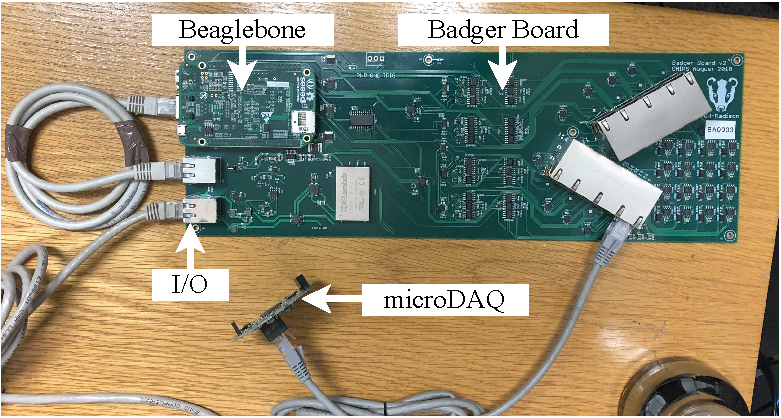
\includegraphics[width=0.8\textwidth]{diagrams/5-daq/madison_plane.pdf}
    \caption[Labelled picture of the components of the Madison \textsc{Pom} electronics box]
    {Labelled picture of the components of the Madison \textsc{Pom} electronics box.}
    \label{fig:madison_plane}
\end{figure}

Similarly, up to 16 Madison \textsc{Pom} badger-boards receive power, networking and WR
synchronised IRIG-B and \unit{10}{\text{MHz}} timing signals from a \emph{danout-board} located
within a single \emph{Madison-container}. Again, standard category 5 cables with RJ45 connectors
are used for these connections. The full contents of the Madison-container are shown in
Fig.~\ref{fig:madison_box}. Similar to the badger-board, the danout-board acts as a simple fanout
and power control board with an attached mezzanine Beaglebone. However, in this case, the attached
Beaglebone acts only to control the power provided by the danout-board.

PMT hits and other packets are instead routed through the danout-board into a networking stack.
Consisting of a WR-LEN, a router (required due to the limited WR-LEN routing table size), and a
switch (non WR), the stack provides networking to the higher-level DAQ via a single optical fibre.
The WR clock synchronised IRIG-B and \unit{10}{\text{MHz}} timing signals are output by the WR-LEN
to the danout-board for forwarding to the lower-level components. Additionally, two AC to DC
converters provide power for both the devices within the container and all lower-level components
via the danout-board.

\begin{figure} % MADISON BOX DIAGRAM %
    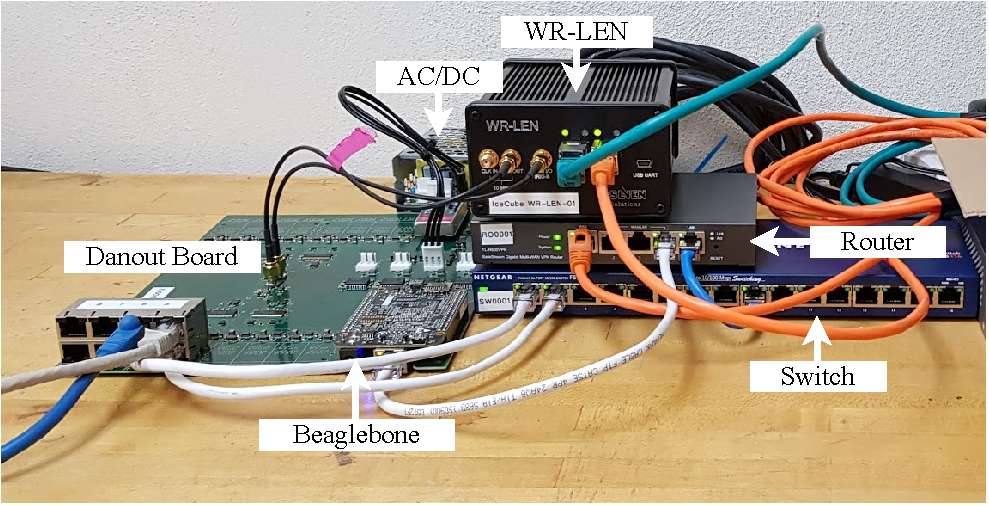
\includegraphics[width=\textwidth]{diagrams/5-daq/madison_box.pdf}
    \caption[Labelled picture of the Madison-container components]
    {Labelled picture of the Madison-container components. The blue and grey cables exiting the
        left hand side of the image go to individual Madison \textsc{Pom}s connecting to the I/O
        port shown in fig.~\ref{fig:madison_plane}. An optical fibre connection into the left SFP
        port of the WR-LEN is used in reality rather than the copper connection shown here.}
    \label{fig:madison_box}
\end{figure}

Compared to the Nikhef hardware the Madison.
\begin{itemize}
    \item By leveraging commercially available Beaglebones ($\sim£50$ each) for onboard logic and
    using vastly \textbf{cheaper} WR-LENs compared to WR switches, the Madison DAQ hardware
    implementation is drastically cheaper compared to the Nikhef (KM3NeT) approach for a minimal
    reduction in performance.
    \item By having a fully fledged Linux machine on each POM and easily reprogrammable
    $\micro$DAQ microcontrollers the DAQ software can be easily \textbf{configurable} and upgraded
    once deployed. Having so much cheap general purpose processing power close to the PMTs allows
    for most of the computation to happen at that level, additional logic can be added. Don't even
    know what we could implement yet using it. Advanced processing at lower level. 
\end{itemize}

\subsection{Combined systems} %%%%%%%%%%%%%%%%%%%%%%%%%%%%%%%%%%%%%%%%%%%%%%%%%%%%%%%%%%%%%%%%%%%%
\label{sec:daq_hard_combined} %%%%%%%%%%%%%%%%%%%%%%%%%%%%%%%%%%%%%%%%%%%%%%%%%%%%%%%%%%%%%%%%%%%%

Each Nikhef-container and Madison-container is connected to a single \emph{junction-box}, labelled
in Fig.~\ref{fig:full_setup}. This central container acts as the interface between the detector
electronics and the umbilical carrying data and power between the shore and the detector. All
connections to the junction-box (as well as those between \textsc{Pom}s and Nikhef and Madison
containers) are made within watertight, flexible PVC tubing called \emph{manifolds}. These tubes
span all corners of the \chipsfive detector, as shown in Fig.~\ref{fig:manifold}.

\begin{figure} % MANIFOLD DIAGRAM %
    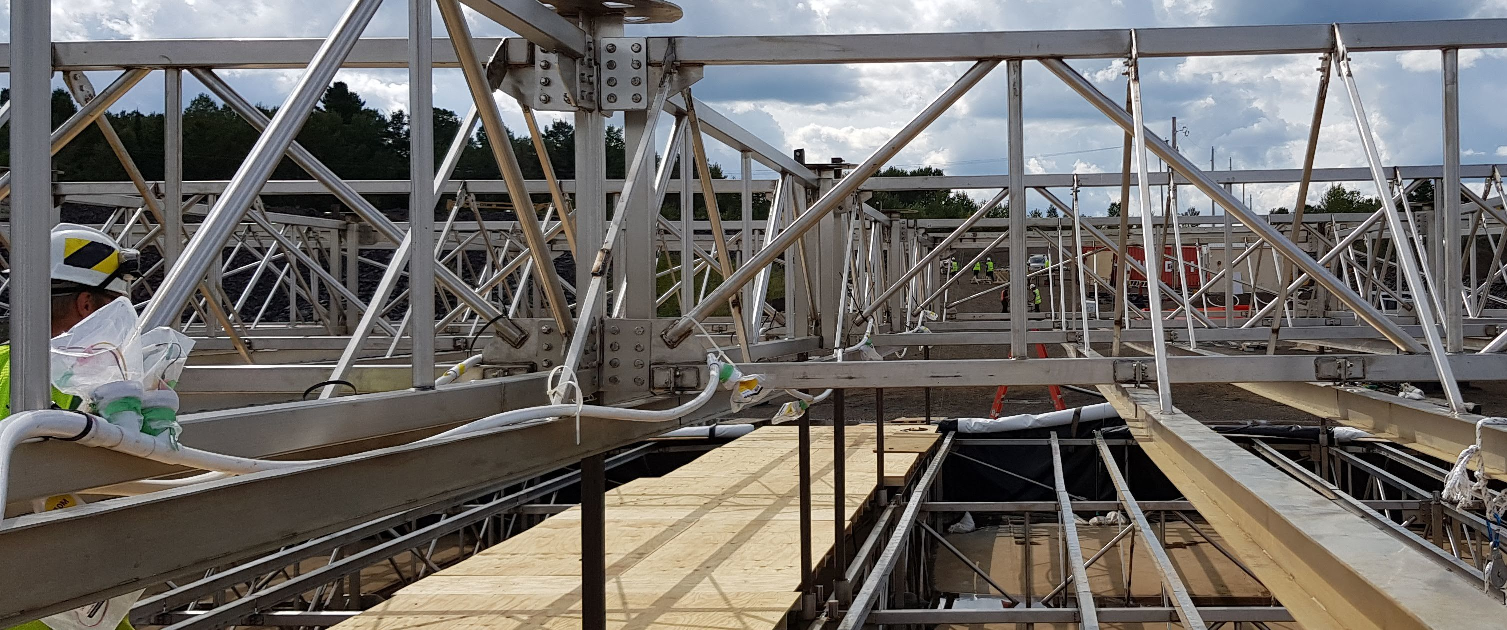
\includegraphics[width=\textwidth]{diagrams/5-daq/manifold.pdf}
    \caption[Picture of a manifold connection within the \chipsfive detector]
    {Picture of a Nikhef \textsc{Pom} to Nikhef-container manifold (in white) attached to the
        top-cap of the \chipsfive detector. In the left of the image, two unattached Nikhef
        \textsc{Pom} pigtail connections are seen, both covered in green tape and a plastic bag.}
    \label{fig:manifold}
\end{figure}

For networking the junction-box contains a Coarse Wavelength Division Multiplexing (CWDM)
multiplexer/demultiplexer (MUX/DEMUX). This device supports 32 wavelengths for a total of 16
bi-directional \unit{1}{\text{Gb}} connections over the single \unit{500}{\text{m}} long umbilical
optical fibre. Each WR-LEN or WR switch within the detector uses one of these channels exclusively
with the corresponding wavelength SFP.

The two umbilical power connections are distributed via two thick copper plates to all the relay
channels within the junction-box. Two relay boards are used to provide a sufficient number of
output channels, with their control electronics powered by separate AC to DC converters and each
connected to one of the multiplexer/demultiplexer networking channels via a media converter
(optical fibre to RJ45). Each relay channel also has a built-in \emph{trip gate} to immediately
power-off the channel if a current surge is detected. This protection is particularly crucial for
\chipsfive as water leaks are possible.

The contents of the DAQ electronics \emph{Shore Hut} are shown in Fig.~\ref{fig:hut_daq}. The
single umbilical optical fibre connection passes through a multiplexer/demultiplexer before each
of the wavelength-specific channels are passed into one of two WR switches. Multiple Virtual Local
Area Networks (VLANs) are configured on each switch such that for each wavelength channel only a
single paired port on the other physical side of the switch carries that channels data to and from
the standard networking switch (these connections are not present within Fig.~\ref{fig:hut_daq}).
Of the two WR switches, one is configured to be the GrandMaster with connections to a GPS
disciplined oscillator with an attached antenna. A single connection is also made between the WR
switches for clock synchronisation.

\begin{figure} % WHITE-RABBIT GM SETUP DIAGRAM %
    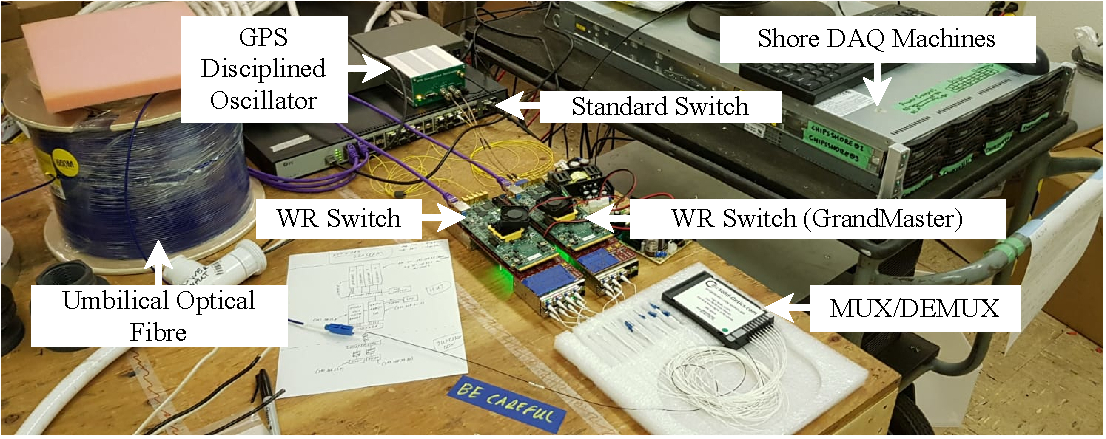
\includegraphics[width=\textwidth]{diagrams/5-daq/hut_daq.pdf}
    \caption[Picture of the onshore components of the \chipsfive DAQ system]
    {Picture of the onshore components of the \chipsfive DAQ system arranged on a table at the
        PolyMet mining administration building.}
    \label{fig:hut_daq}
\end{figure}

The standard network switch provides \unit{10}{\text{Gb}} connections to each of the Shore DAQ
computing machines whose specific roles are detailed in Section.~\ref{sec:daq_soft}. Each machine
is also connected to a second switch providing connections to the external internet and DAQ
components located at Fermilab. At Fermilab, a principle DAQ machine (Fermi DAQ-1) performs two
main roles. Firstly, it forwards \numi beam spill timing information from a Time Distribution Unit
attached to the Main Injector clock to \chipsfive. Secondly, it receives recorded detector data
from the \chipsfive located DAQ system and places it into long-term storage.

An uninterruptible power supply provides power to all devices within the Shore Hut, supplying
power for up to \unit{15}{\text{minutes}} after a power cut (sadly quite a common occurrence). The
two detector umbilical power connections do not use the uninterruptible supply and instead draw
power directly from the master supply, as does the water filtration pump.

\section{Software} %%%%%%%%%%%%%%%%%%%%%%%%%%%%%%%%%%%%%%%%%%%%%%%%%%%%%%%%%%%%%%%%%%%%%%%%%%%%%%%
\label{sec:daq_soft} %%%%%%%%%%%%%%%%%%%%%%%%%%%%%%%%%%%%%%%%%%%%%%%%%%%%%%%%%%%%%%%%%%%%%%%%%%%%%

The software of the \chipsfive DAQ system provides three main functionalities: control of the
detector instrumentation, the handling of recorded PMT hits, and the monitoring of hardware and
data quality. Each of these functions is discussed within a specific subsection below. Only the
high-level software components are detailed with the low-level CLB, Beaglebone, and $\micro$DAQ
software implementations omitted for brevity. An in-depth discussion of the CLB software can be
found in Ref.~\cite{aiello2019} while the Beaglebone and $\micro$DAQ software implementation can
be found at Ref.~\cite{microdaq2020}.

\begin{figure} % SOFTWARE DIAGRAM %
    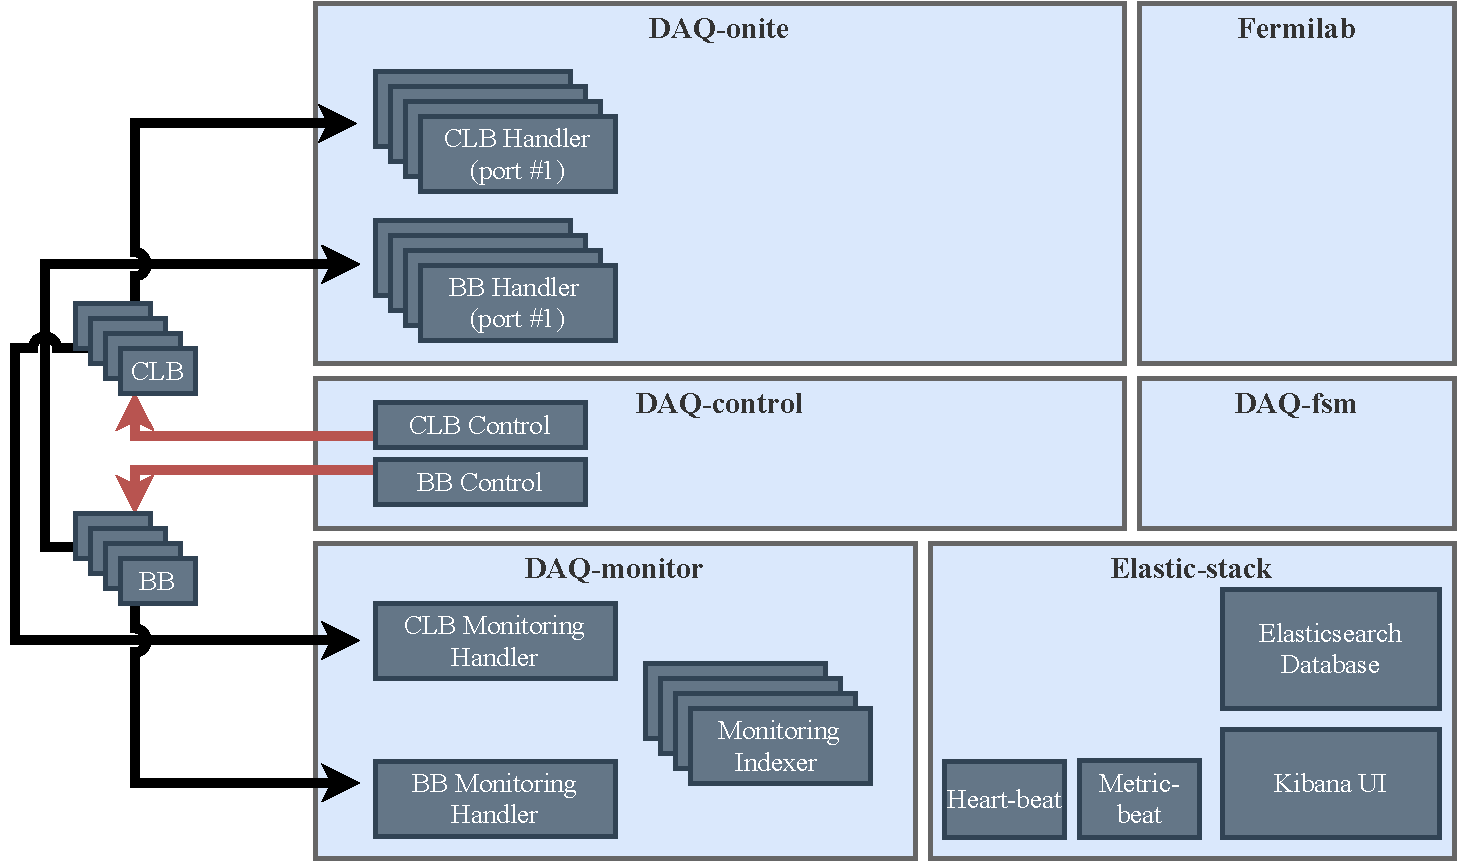
\includegraphics[width=\textwidth]{diagrams/5-daq/daq_software.pdf}
    \caption[Diagram of the \chipsfive software system in terms of the flow of data between
    components] {Diagram of the \chipsfive software system in terms of the flow of data between
    high-level components.}
    \label{fig:daq_software}
\end{figure}

The software itself is mainly written in C++ and can be found in the repository at
Ref.~\cite{chipsdaq2020}. The complete system is comprised of multiple processes, each of which is
illustratively shown within Fig.~\ref{fig:daq_software}, expressed in terms of the flow of data
between distinct software components. All DAQ processes make extensive use of multithreading and
asynchronous communication, principally implemented using the low-level Boost Asio (asynchronous
input/output) library~\cite{boost2020}. 

All central processing takes place on one of three machines: Shore DAQ-1 for hit handling, Shore
DAQ-2 control and monitoring, and Fermi DAQ-1 for \numi spill forwarding and storage. As the
processing of PMT hits is the principle software task, handled takes place exclusively on Shore
DAQ-1 without other processes to ensure maximum available processing power. Both Shore DAQ
machines have a backup machine (Shore DAQ-3 and Shore DAQ-4) to take over their functions in case
of a fault.

\subsection{Detector control} %%%%%%%%%%%%%%%%%%%%%%%%%%%%%%%%%%%%%%%%%%%%%%%%%%%%%%%%%%%%%%%%%%%%
\label{sec:daq_soft_control} %%%%%%%%%%%%%%%%%%%%%%%%%%%%%%%%%%%%%%%%%%%%%%%%%%%%%%%%%%%%%%%%%%%%%

All DAQ processes are controlled by a singular Finite State Machine (FSM) process. The FSM can be
in exactly one 

\begin{figure} % SOFTWARE DIAGRAM %
    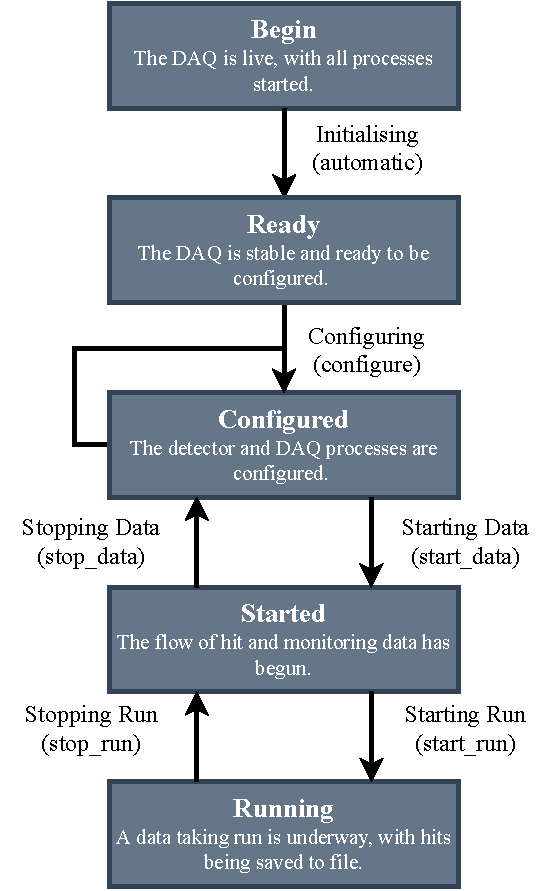
\includegraphics[width=0.6\textwidth]{diagrams/5-daq/fsm.pdf}
    \caption[fsm]
    {fsm}
    \label{fig:fsm}
\end{figure}

- inspired by the KM3NeT Java implementation
A singular Finite State Machine (FSM) process on DAQ
- Finite State Machine (FSM)
- DHCP server controls all the static ip addresses!
- Sometimes referred to as slow-control
- typically this is separated physically into a separate network, that is the best way to do the
DAQ for multiple reasons, but this would make the \chips DAQ system dramatically more complicated,
as running another cable requires so much more effort than normal, so they are combined into one.
- The detector is configured using a single human readable configuration file that defines all the
\textsc{Pom} types, MAC addresses, IP addresses, types, relay channels, which channels should be active and
their associate high voltage setting, threshold and electronic ID.
- Taking inspiration from the KM3NeT DAQ Java software
- Currently no run control system is in place to automatically control the detector according to a
scheduled run plan. Detector control is done via a simple command line interface (CLI) that
communicates with the FSM. Starting data taking, starting runs of a given type, stopping,
configuring with a given configuration file etc...

\subsection{Hit acquisition} %%%%%%%%%%%%%%%%%%%%%%%%%%%%%%%%%%%%%%%%%%%%%%%%%%%%%%%%%%%%%%%%%%%%%
\label{sec:daq_soft_hits} %%%%%%%%%%%%%%%%%%%%%%%%%%%%%%%%%%%%%%%%%%%%%%%%%%%%%%%%%%%%%%%%%%%%%%%%

As in done within KM3NeT, an `all-data-to-shore' approach is taken, where all PMT hit data is sent
via the WR network to the machines on shore. No triggering takes place within the detector. This
is done by collecting all PMT hits on each low level device (CLB or Beaglebone) within time
windows, \unit{10}{\mathrm{ms}} in length. At the end of each window, data is packaged along with
a header into User Datagram Protocol (UDP) packets and sent to shore. 

UDPavoids the overhead of error checking and correction processes, as this should be low it is not
required as allows for a higher bandwidth data stream to shore.

- How the beam spill stuffy works and how it is used to trigger hit acquisition
- Talk about the data rates for hits at full steam
- Jumbo frames etc
- Data is sent in UDP packets (not TCP so some will go missing)
- Typical ethernet frame has a maximum transmission unit (MTU) size of 1500 bytes, we use Jumbo
frames that allow for an MTU of 9000 bytes, this means we have a lot less small frames with only a
limited number of recorded hits, which proved to be taxing to the switches and lead to an increase
in the number of dropped frames.
- 1Gb links between WR switches, 10Gb link between FS switch and main DAQ machine. Provides
sufficient bandwidth, DO A SMALL CALCULATION!

\subsection{Monitoring} %%%%%%%%%%%%%%%%%%%%%%%%%%%%%%%%%%%%%%%%%%%%%%%%%%%%%%%%%%%%%%%%%%%%%%%%%%
\label{sec:daq_soft_monitor} %%%%%%%%%%%%%%%%%%%%%%%%%%%%%%%%%%%%%%%%%%%%%%%%%%%%%%%%%%%%%%%%%%%%%

- Talk about the data rates for monitoring at full steam
- Which machines run this, which is backup?

- Elasticsearch ref in~\cite{elastic2020}
- An open source RESTful, JSON-based, search engine and noSQL database.
- Data is stored in \emph{indices} in individual \emph{documents}
- Get to leverage an enormous amount of online support and the community
- daqlog: Uses for DAQ application logging with a severity
- daqstate: Used to report the current state of various DAQ applications
- monpom: Used for reporting general \textsc{Pom} monitoring information, such as temp, humidity, status
- monchannel: Used for reporting individual channel monitoring, such as rate, veto
- A series of altering rules are also set up constantly monitoring the status of the monitoring
data contained within the elasticsearch database to alert via slack or email individuals if something goes wrong.
- We index asynchronously to not block data taking, all data is backed up easily.
- Use the Kibana user interface which is accessible through a browser, means that no special
equipment, or GUIs are used, anyone on any machine has access to the full monitoring stack from
their browser. A series of dashboards ar set up to monitor everything within the detector.
- A series of indices are set up to store data which is sent via standard REST messages to the
database, the special indexing allows for quick `searching' over any time period etc... for
monitoring.
- Also means that anyone can quickly/easily look at any part of the data and make plots etc...
without needing to write an additional part of a monitoring program.
- Means the full detector and data quality monitoring is accessible to anyone with access anywhere
in the world via their normal browser.

\begin{figure} % MONITORING DIAGRAM %
    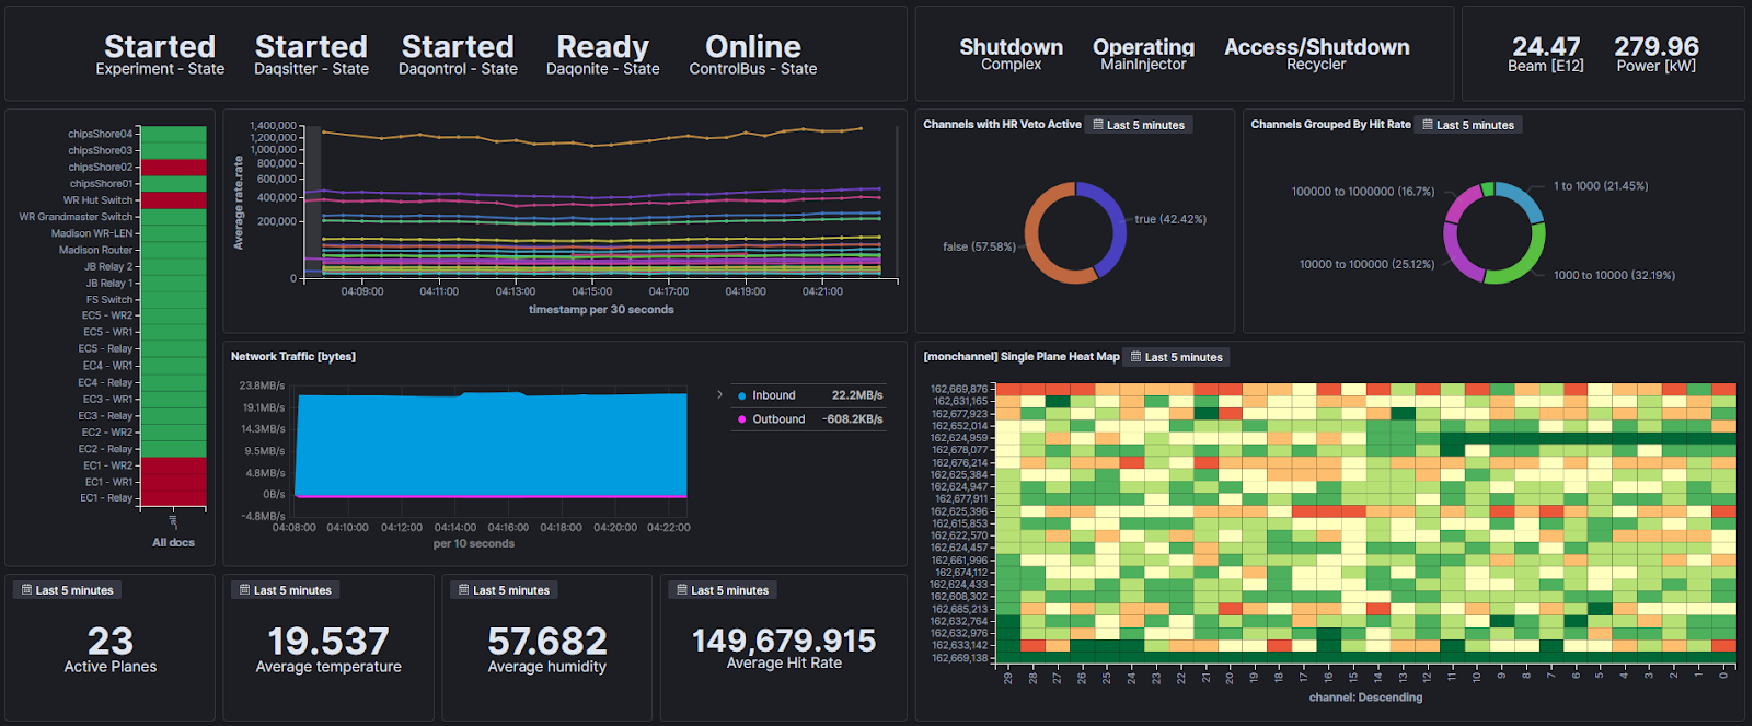
\includegraphics[width=\textwidth]{diagrams/5-daq/monitoring.pdf}
    \caption[monitoring short]
    {monitoring long}
    \label{fig:monitoring}
\end{figure}
    \chapter{Convolutional neural networks for CHIPS} %%%%%%%%%%%%%%%%%%%%%%%%%%%%%%%%%%%%%%%%%%%%%%%%
\label{chap:cnn} %%%%%%%%%%%%%%%%%%%%%%%%%%%%%%%%%%%%%%%%%%%%%%%%%%%%%%%%%%%%%%%%%%%%%%%%%%%%%%%%%

For the majority of HEP experiments, event analysis entails the separation of signal from
background, the identification of particle types, the discovery of spatial properties, and the
estimation of energies. The same is true for \chips detectors, with the primary aims being the
selection of appeared CC $\nu_{e}$ signal events from a sizeable background, and the estimation of
associated neutrino energies.

For this purpose, the \chips project has so far relied on a human implemented reconstruction
algorithm and a simple classification neural network driven by hand-engineered features. Both are
prone to human error and restricted in scope to what has been implemented in software.

The work outlined in this chapter presents a replacement event analysis methodology for \chips.
Three \emph{Convolutional Neural Networks} (CNNs)~\cite{fukushima1982}, a type of \emph{deep
learning}~\cite{goodfellow2016} neural network have been implemented to achieve the primary aims
outlined above amongst others. One for cosmic rejection, one for beam classification, and one for
neutrino energy estimation. For evaluation purposes, only the implementation as applied to the
\chipsfive detector module is considered in this work.

After mentioning previous implementations of deep learning for neutrino experiments, a description
of the current (standard) techniques is given. The theoretical background of CNNs is then outlined
before the baseline implementation for \chips is described. The specific implementations for each
of the three networks are then discussed with a comprehensive evaluation of their performance and
behaviour presented separately in the following chapter (Chapter.~\ref{chap:results}).

\section{Previous applications of deep learning for neutrino experiments} %%%%%%%%%%%%%%%%%%%%%%%%
\label{sec:cnn_previous} %%%%%%%%%%%%%%%%%%%%%%%%%%%%%%%%%%%%%%%%%%%%%%%%%%%%%%%%%%%%%%%%%%%%%%%%%

Over the last few years, neutrino experiments have started to adopt deep learning techniques for a
range of event analysis tasks~\cite{psihas2020}. This trend has closely followed the general
explosion of interest in the field amongst the global research community, especially within the
sub-field of computer vision, as can be seen in Fig.~\ref{fig:papers}.

\begin{figure} % NUMBER OF PAPERS DIAGRAM DIAGRAM %
    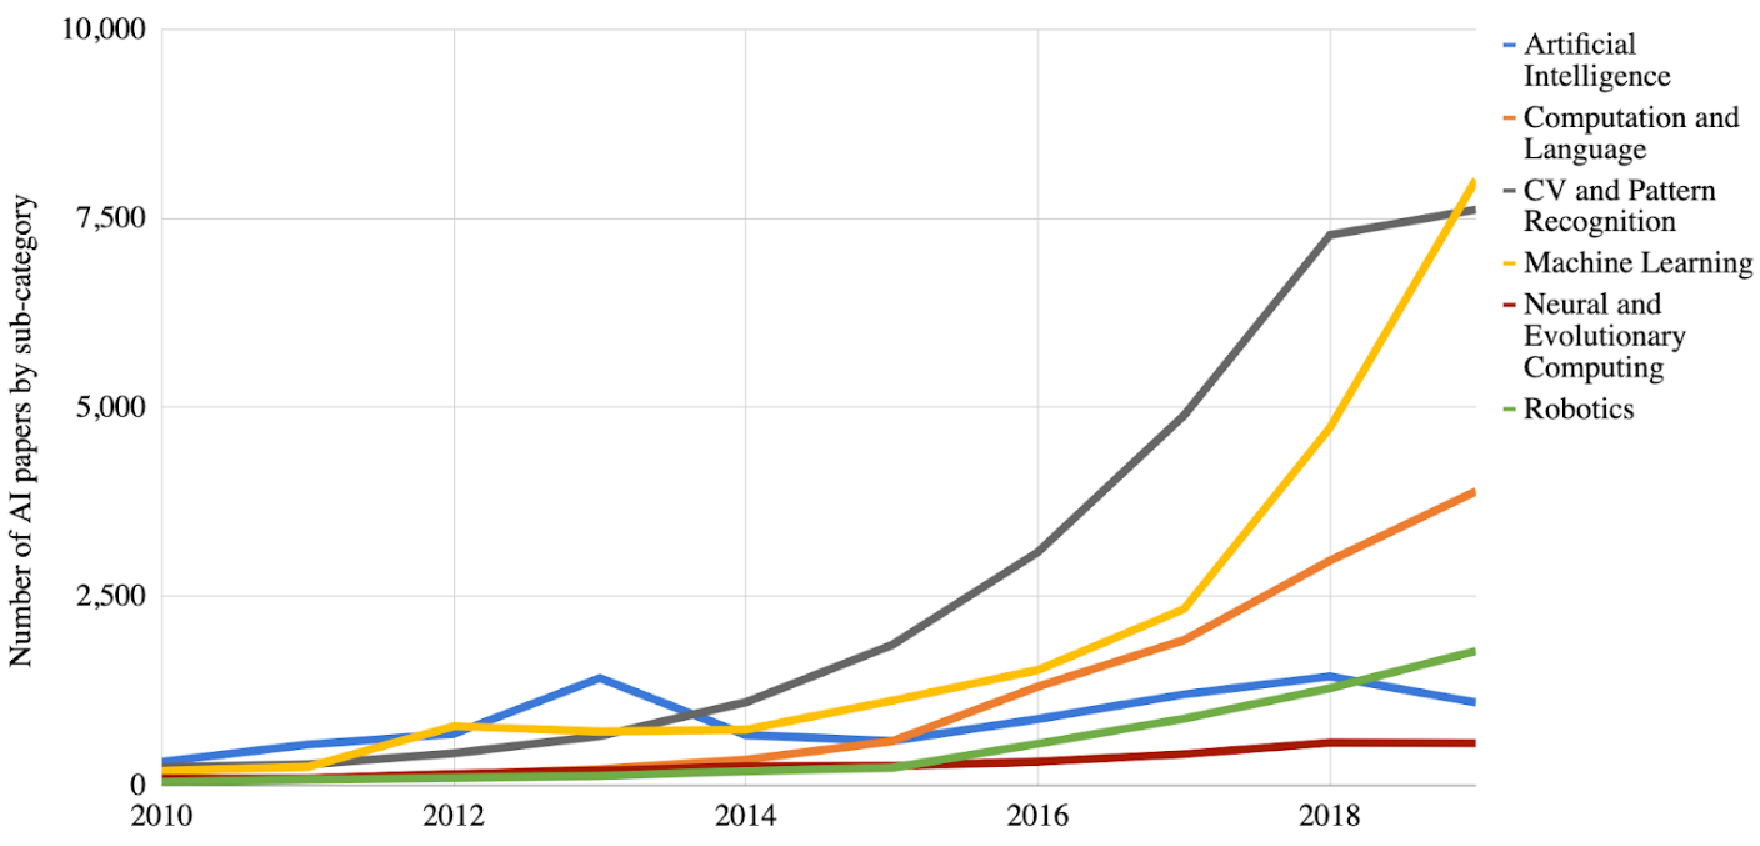
\includegraphics[width=0.8\textwidth]{diagrams/6-cnn/papers.pdf}
    \caption[The number of artificial intelligence papers submitted to arXiv]
    {The number of artificial intelligence papers submitted to arXiv, broken down by sub-category.
        Note the particularly large increase in Computer Vision (CV) and pattern recognition
        papers. Figure taken from Ref.~\cite{perrault2019}.}
    \label{fig:papers}
\end{figure}

In 2016 the \nova experiment applied a CNN to the task of classifying the interaction type of
events within their sampling calorimeter detector~\cite{aurisano2016}. Two views of raw detector
data were used as input to train a network based on the popular GoogLeNet
architecture~\cite{szegedy2015} (discussed in Section.~\ref{sec:cnn_theory_conv}). Further \nova
iterations have since been applied to both the classification of individual energy deposit
clusters~\cite{psihas2019} and $\nu_{e}$ and $e^{-}$ energy reconstruction~\cite{baldi2019}.

CNNs have also been applied to liquid argon time-projection chambers. The MicroBooNE
experiment~\cite{acciarri2017_ref} has shown that in addition to classification tasks, the spatial
localisation of single particles within events is possible~\cite{acciarri2017}. Furthermore, the
DUNE collaboration has designed a network to output both the interaction class and counts of
different particle types within an event~\cite{collaboration2020, abi2020}. This approach taken by
DUNE is called \emph{multi-task} learning and is discussed in detail within
Section.~\ref{sec:cnn_baseline_outputs}.

Applications to water Cherenkov detectors have also been made by both the Daya Bay
experiment~\cite{racah2016} and the KM3NeT/ORCA collaboration~\cite{aiello2020}. Furthermore, a
type of CNN known as a \emph{variational autoencoder} has been shown to approximate the
distribution of simulated water Cherenkov data well~\cite{abhishek2019}. If further such studies
prove successful, this could allow for training on `real' data to mitigate experimental
uncertainties and vastly increase the speed of simulated data generation.

\section{Standard event reconstruction and classification} %%%%%%%%%%%%%%%%%%%%%%%%%%%%%%%%%%%%%%%
\label{sec:cnn_old} %%%%%%%%%%%%%%%%%%%%%%%%%%%%%%%%%%%%%%%%%%%%%%%%%%%%%%%%%%%%%%%%%%%%%%%%%%%%%%

It is essential to outline the standard event reconstruction and classification methods used by
the \chips project until now. This is for two reasons. Firstly, to highlight their main weaknesses
as motivation for the new CNN approach. Secondly, to provide context for the performance
comparisons made in Chapter.~\ref{chap:results}.

A likelihood method based on that implemented by MiniBooNE~\cite{patterson2009} is used for event
reconstruction, while a simple neural network built using the TMVA package~\cite{hocker2007} is
used for event classification. Both methods are representative of the mainstream approach used by
the majority of water Cherenkov neutrino experiments for event analysis. A prime example is the
fiTQun algorithm developed for the Super-Kamiokande detector, used for both
atmospheric~\cite{jiang2019} and T2K~\cite{missert2017} analyses.

\subsection{Likelihood based reconstruction} %%%%%%%%%%%%%%%%%%%%%%%%%%%%%%%%%%%%%%%%%%%%%%%%%%%%%
\label{sec:cnn_old_reco} %%%%%%%%%%%%%%%%%%%%%%%%%%%%%%%%%%%%%%%%%%%%%%%%%%%%%%%%%%%%%%%%%%%%%%%%%

The event reconstruction methodology is simple in theory: for a given set of hypothesised charged
particle tracks, the number of Cherenkov photoelectrons and the time at which the first of these
is recorded for each PMT in the detector is predicted. By comparing this prediction with the
measured hit charges and times the likelihood that the given track hypothesis produced the
measured signals can be calculated. The parameters that describe the hypothesised tracks are then
varied until the negative logarithm of the likelihood is minimised, identifying the best-fit
parameters. A brief description of the full procedure is given below, however, for a detailed
description see Ref.~\cite{blake2016} and Ref.~\cite{perch2017}. The full C++ software
implementation can also be found in the repository at Ref.~\cite{chipsreco2020}.

\subsubsection*{Seeding} %%%%%%%%%%%%%%%%%%%%%%%%%%%%%%%%%%%%%%%%%%%%%%%%%%%%%%%%%%%%%%%%%%%%%%%%%

The first stage of event reconstruction is the effective \emph{seeding} of tracks that are then
used in the full likelihood fit. The seeding methods aim to provide a good starting point for the
minimisation, both to increase the efficiency of finding the optimal track parameters and also to
avoid a false local minimum from being returned.

Firstly, the PMT hits are sliced in both space and time. Gaps in the time ordering of hits are
used to separate the event into time slices. Each of these slices then undergoes basic filtering
and clustering to remove outlying hits and ensure only the dominant collections of hits are
considered. Each cleaned slice is then run through simple geometric vertex finding algorithms to
estimate the interaction position and time, in addition to the initial track direction.

A circular \emph{Hough transform} algorithm, traditionally used for water Cherenkov ring finding
is then applied. As output, the voting-based transformation produces a space within which rings of
PMT hits exist as peaks. The track direction values are further refined using this space before a
search for secondary peaks is carried out to indicate if multiple particles are likely to be
involved. This process results in a list of seeds, each with a score related directly to the
height of the associated peak in Hough transform space.

\subsubsection*{Likelihood fit} %%%%%%%%%%%%%%%%%%%%%%%%%%%%%%%%%%%%%%%%%%%%%%%%%%%%%%%%%%%%%%%%%%


Each particle track in a fit hypothesis comprises a vector of parameters $\vec{x}$, containing the
following:
\begin{itemize}
    \item the track interaction vertex position ($x_{0}$, $y_{0}$, $z_{0}$) and time ($t_{0}$);
    \item the initial track direction ($d_{\theta}$, $d_{\phi}$);
    \item the initial kinetic energy of the particle ($E_{k}$); and
    \item the particle type (muon, electron or photon).
\end{itemize}
For a photon hypothesis (identical to an electron hypothesis in reality) the distance between the
interaction vertex and the beginning of the electromagnetic shower is also included as a
parameter.

The hypothesised tracks are then initialised using the list of seeds found in the seeding
procedure in descending order of Hough peak height score. As the seeding algorithms do not
estimate the particle energy, a default value equal to the average particle energy observed in the
Monte Carlo simulation is assigned. Additionally, constraints can be placed on a multi-track
hypothesis to reduce the number of free parameters.

As an example, consider the NC $\pi^{0}$ case, where a multi-track two-photon hypothesis is used.
Firstly, the initial parameters for the two photons are assigned from the two highest-scoring
seeds from the seeding procedure. Secondly, the vertex position for both tracks is constrained to
remain the same, and the directions and energies are set to be constrained by the invariant mass
of the $\pi^{0}$.

In it's simplest form the likelihood $\mathcal{L}(\vec{x})$, is a simple product of two terms:
\begin{equation} % LIKELIHOOD EQUATION %
    \mathcal{L}(\vec{x})=\mathcal{L}_{unhit}(\vec{x})\mathcal{L}_{hit}(\vec{x})=
    \prod_{unhit}P_{unhit}(\vec{x})\prod_{hit}P_{charge}(\vec{x})P_{time}(\vec{x}),
    \label{eq:likelihood}
\end{equation}
where the first ($unhit$) term gives the likelihood that the hypothesis $\vec{x}$ will not predict
a hit on the PMTs that do not have a measured hit, and the second ($hit$) term gives the
likelihood that $\vec{x}$ produces the observed photoelectrons and hit times on the measured hit
PMTs. 

By considering the negative logarithm of the likelihood the computation can be simplified into a
sum of logarithms over the PMTs, such that
\begin{equation} % LIKELIHOOD SUM PMTS EQUATION %
    -\log\mathcal{L}(\vec{x})=
    -\sum_{unhit}\log(P_{unhit}(\vec{x}))
    -\sum_{hit}\log(P_{charge}(\vec{x}))
    -\sum_{hit}\log(P_{time}(\vec{x})).
    \label{eq:likelihood_sum}
\end{equation}
This form has the effect of separating the charge (number of photoelectrons) and time prediction
components, which can then be dealt with separately computationally. In the actual likelihood
calculation the $P_{unhit}(\vec{x})$ and $P_{charge}(\vec{x})$ components are combined, where the
probability of an unhit PMT is treated as a PMT with an observed charge equal to zero.

The Minuit2 algorithm contained within the ROOT software package~\cite{brun1997} is used for the
minimisation process. At each iteration, the charge and hit time predictions are made, and the
negative logarithm of the likelihood is calculated. The track parameters are then varied to
minimise the likelihood before the next iteration begins. Through a series of stages, each fixing
and freeing specific parameters, the minimisation process converges to the best-fit parameters for
the given hypothesis. This procedure typically takes two minutes on a standard batch farm
computing node.

\subsubsection*{Downsides} %%%%%%%%%%%%%%%%%%%%%%%%%%%%%%%%%%%%%%%%%%%%%%%%%%%%%%%%%%%%%%%%%%%%%%%

The charge and hit time predictions and their associated likelihood contributions depend on many
low-level inputs. Generally, these inputs describe how Cherenkov light is emitted from specific
particles and how it propagates through the detector to be detected by the PMTs. Examples of these
inputs include:
\begin{itemize}
    \item the number of Cherenkov photons emitted by a particle of a specific type and energy;
    \item the fraction of Cherenkov light emitted at each step along a specific particle's track
          length;
    \item the angular distribution of Cherenkov photon emission for each type of particle;
    \item the survival probability of photons within the detector medium as a function of distance
          and energy;
    \item a detailed description of the PMT positions and directions;
    \item the angular efficiency of each PMT relative to the incident photon angle; and
    \item the probability of a measured charge given the predicted number of photoelectrons (see
          Fig.~\ref{fig:digi_likelihood}).
\end{itemize}

The above list demonstrates a fundamental problem with the likelihood based approach. Namely, it
is heavily reliant on the accuracy of multiple low-level inputs and their associated use in human
implemented software. If a physical process is not modelled appropriately or more crucially
overlooked (such as the hadronic component of neutrino events is here), then the prediction
accuracy of PMT charges and hit times is affected, impacting the performance of the best-fit
parameters.

Moreover, the likelihood based approach requires a predefined track hypothesis per fit. This
restriction is at odds with the broad array of neutrino events expected within \chips detector
modules. Many possible combinations of final state particles are possible, making the
implementation of an approach where all possible events are considered, challenging. For example,
the very similar Super-Kamiokande fiTQun algorithm attempts multiple fits for each event,
sequentially adding charged particles to the hypothesis until the best-fit is found. This
technique vastly increases the time required to analyse a single event, still ignores some
possible scenarios, and can never be fully rigorous.

\subsection{Event classification}%%%%%%%%%%%%%%%%%%%%%%%%%%%%%%%%%%%%%%%%%%%%%%%%%%%%%%%%%%%%%%%%%
\label{sec:cnn_old_pid} %%%%%%%%%%%%%%%%%%%%%%%%%%%%%%%%%%%%%%%%%%%%%%%%%%%%%%%%%%%%%%%%%%%%%%%%%%

As the standard event reconstruction is based on the calculation of a likelihood (analogous to a
goodness-of-fit), the likelihood ratio between different hypotheses can be used for event
classification tasks. Additional hand-engineered features derived from the reconstruction outputs
are also found to have power in classifying the event type.

Two simple neural networks are used, the first for CC $\nu_{e}$ - CC $\nu_{\mu}$ separation and
the second for CC $\nu_{e}$ - NC separation. Both contain a single hidden layer (as described in
the following Section.~\ref{sec:cnn_theory}) with the number of neurons equal to the number of
input parameters plus five. Output variables from both a single electron track and single muon
track hypothesis fit to each event are used for both networks, including:
\begin{itemize}
    \item the $\Delta\log\mathcal{L}$ between $e$ and $\mu$ hypothesis for both time and charge
          components;
    \item the total number of hit PMTs ($N_{hits}$) and total collected charge;
    \item $\frac{\Delta\log\mathcal{L}_{charge}}{N_{hits}}$;
    \item the fraction of hits inside, within, and outside the ring for both the $e$ and $\mu$
          hypotheses;
    \item the fraction of predicted charge outside the ring for both the $e$ and $\mu$ hypotheses;
    \item the ratio of the total predicted charged to the total measured charge for both the $e$
          and $\mu$ hypothesis;
    \item the ratio of the reconstructed energy to the total measured charge;
    \item the reconstructed track direction under the $e$ hypothesis;
    \item the fraction of hits in the downstream half of the detector;
    \item the number of seeds generated by the Hough transform seeding algorithm; and
    \item the peak height score of the first and last seeds found by the Hough transform seeding
          algorithm.
\end{itemize}

A sample of CC $\nu_{e}$ and CC $\nu_{\mu}$ beam events characteristic of those expected to be
seen within \chipsfive are used to train the first classifier, and a corresponding sample of CC
$\nu_{e}$ and NC events for the second. The output values from both networks can then be used to
select CC $\nu_{e}$ events from the background. Note that only the selection of CC $\nu_{e}$
events has been implemented, no CC $\nu_{\mu}$ selection has been developed.

The principal limitation of this approach is that the input features are restricted to those that
have been imagined (requiring extensive domain knowledge) and then implemented in software. The
current list is undoubtedly non-exhaustive of all the possible variables and combinations of
variables that can, in theory, be used for discrimination between events. Additionally, any
mistakes in the likelihood based reconstruction and, therefore, input variables to the neural
networks, can lead to incorrect classification of events.

\section{The theory of neural networks} %%%%%%%%%%%%%%%%%%%%%%%%%%%%%%%%%%%%%%%%%%%%%%%%%%%%%%%%%%
\label{sec:cnn_theory} %%%%%%%%%%%%%%%%%%%%%%%%%%%%%%%%%%%%%%%%%%%%%%%%%%%%%%%%%%%%%%%%%%%%%%%%%%%

There are many machine learning techniques: linear regression, logistic regression, k-nearest
neighbours, decision trees, random forests, support vector machines, amongst others, all of which
learn to make predictions about data. However, none has been as successful, especially in recent
years, as the deep neural network. As both the size of datasets and the amount of available
computing power has increased, deep neural networks have proved incredibly powerful for many
tasks, as they are well suited to this paradigm.

Here we discuss the application of neural networks for \emph{supervised learning}, one of two
broad machine learning categories concerned with using labelled example data to train algorithms.
The other broad category of \emph{unsupervised learning}, where the properties of the dataset are
inferred without labelled data is not discussed, however, will be used for network
\emph{explainability} in Section.~\ref{sec:results_explain}.

\subsection{Neural network basics} %%%%%%%%%%%%%%%%%%%%%%%%%%%%%%%%%%%%%%%%%%%%%%%%%%%%%%%%%%%%%%%
\label{sec:cnn_theory_basics} %%%%%%%%%%%%%%%%%%%%%%%%%%%%%%%%%%%%%%%%%%%%%%%%%%%%%%%%%%%%%%%%%%%%

A neural network is a type of algorithm inspired by the repeating cell structure of neurons within
our brains. The basic building block of a neural network is a \emph{neuron}, which takes a vector
of $k$ inputs $\vec{x}=(x_{1}, x_{2},\dots,x_{k})$ and outputs a scalar $a(\vec{x})$. Individual
neurons are arranged into layers, with the input of one layer being the output from the previous
layer. The first layer is commonly referred to as the \emph{input layer}, the middle layers as
\emph{hidden layers}, and the final layer as the \emph{output layer}, as illustrated in
Fig.~\ref{fig:network}. In general, this simple neural network structure is referred to as
\emph{fully-connected}, as all the neurons in each layer have connections to all the neurons in
the previous and following layers.

\begin{figure} % BASIC NETWORK DIAGRAM %
    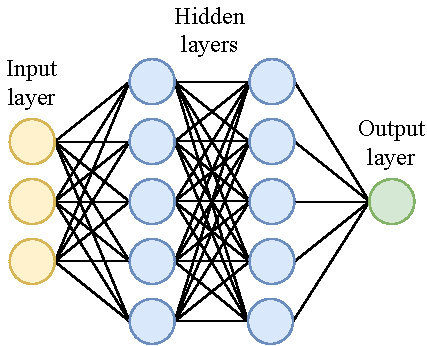
\includegraphics[width=0.6\textwidth]{diagrams/6-cnn/network.pdf}
    \caption[Illustration of a simple neural network]
    {Illustration of a simple neural network. There is a single input layer (yellow), two hidden
        layers (blue), and an output layer (green). Each node corresponds to a \emph{neuron}
        except for the input layer.}
    \label{fig:network}
\end{figure}

Input variables (traditionally hand-engineered features extracted from the raw data) are passed
into the network via the input layer. Any number of hidden layers containing any number of neurons
can then follow. The neurons contained within these layers are trained so that collectively their
$a(\vec{x})$ functions solve the task at hand. For a regression task, the output layer returns a
continuous decimal value. Conversely, for a classification task, a probability value between zero
and one is output for each class. The forward passing of information from one layer to the next is
why neural networks can also be referred to as \emph{feed-forward graphs}.

For a neuron $i$, $a_{i}(\vec{x})$ can be decomposed into a neuron specific linear operation,
followed by a non-linear operation, which is the same across all neurons. The linear operation
consists of the dot product of the input vector $\vec{x}$ with a vector of weights
$\vec{w}^{(i)}=(w_{1}^{(i)}, w_{2}^{(i)},\dots,w_{k}^{(i)})$, plus a bias term $b^{(i)}$:
\begin{equation} % NETWORK BASIC EQUATION %
    z^{(i)}=\vec{w}^{(i)}\cdot\vec{x}+b^{(i)}.
    \label{eq:network}
\end{equation}
After applying the non-linear operation $\sigma_{i}$, commonly referred to as the \emph{activation
    function}, the final neuron output can be written as
\begin{equation} % NETWORK ACTIVATION EQUATION %
    a_{i}(\vec{x})=\sigma_{i}(z^{(i)}).
    \label{eq:activation}
\end{equation}

Traditionally, a step-function (for networks called \emph{perceptrons}) was used for the
activation function. However, as is shown in Section.~\ref{sec:cnn_theory_training}, a non-zero
gradient (only valid at $x=0$ for a step-function) is required for the practical training of
neural networks. In fact, the choice of activation function can greatly affect how the network
trains and performs.

Therefore, common activation function choices have been the \emph{hyperbolic tangent} and the
\emph{sigmoid} functions, primarily because they are bounded and differentiable at all points.
Recently, the \emph{ReLU} and other similar functions have become popular, mainly due to their
avoidance of \emph{vanishing} gradients which occur when the tanh and sigmoid functions become
saturated at large values of $x$. All of these functions are shown in Fig.~\ref{fig:activations}
for reference.

\begin{figure} % ACTIVATIONS DIAGRAM %
    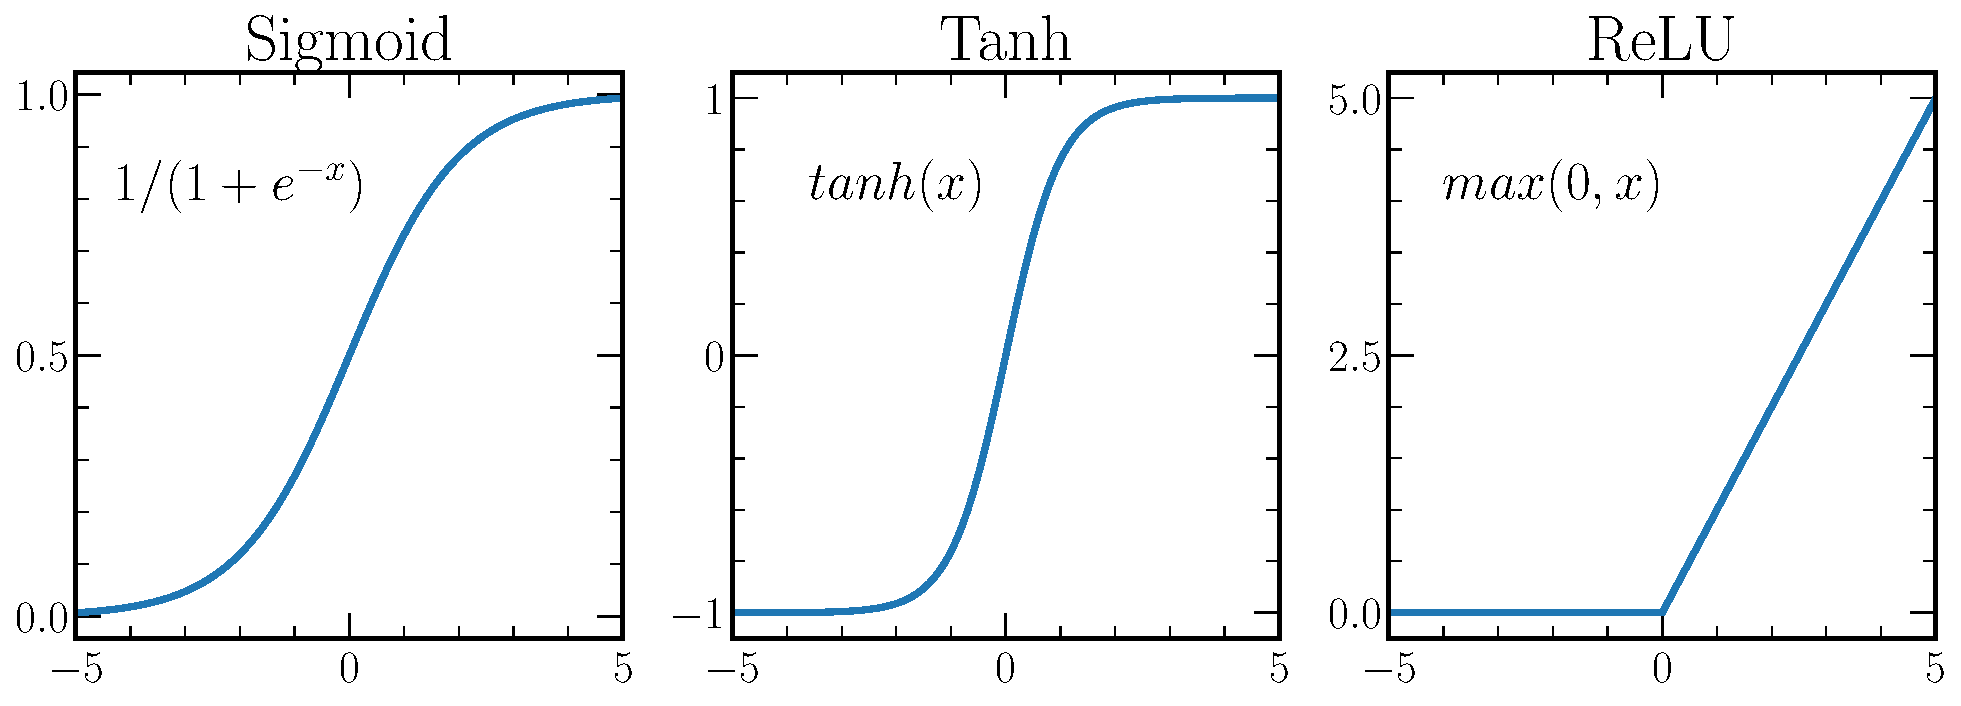
\includegraphics[width=\textwidth]{diagrams/6-cnn/activations.pdf}
    \caption[Common non-linear activation functions]
    {Common non-linear activation functions used for the neurons within neural networks.}
    \label{fig:activations}
\end{figure}

\subsection{Training neural networks} %%%%%%%%%%%%%%%%%%%%%%%%%%%%%%%%%%%%%%%%%%%%%%%%%%%%%%%%%%%%
\label{sec:cnn_theory_training} %%%%%%%%%%%%%%%%%%%%%%%%%%%%%%%%%%%%%%%%%%%%%%%%%%%%%%%%%%%%%%%%%%

Supervised neural network training uses labelled example data to iteratively find the optimal
weights and biases (the network parameters) to maximise output performance. A \emph{loss function}
$E(\vec{w})$ is defined to quantify the difference between the network output and truth label for
each example, where $\vec{w}$ is the vector of network parameters. For a given input example
$(\vec{x}_{i}, y_{i})$, with $\vec{x}_{i}$ being the input parameters and $y_{i}$ the known truth
label, the network generates an output $\hat{y}_{i}(\vec{w})$. Using this notation, we can
construct loss functions suitable for different tasks.

In the case of simple binary classification the most commonly used function is the \emph{binary
cross-entropy}, where
\begin{equation} % BINARY CROSS-ENTROPY EQUATION %
    E(\vec{w})=
    -\displaystyle\sum_{i=1}^{n}y_{i}\log\hat{y}_{i}(\vec{w})+
    (1-y_{i})\log[1-\hat{y}_{i}(\vec{w})],
    \label{eq:binary_cross_entropy}
\end{equation}
with the number of examples given by $n$. For a classification task where the number of classes is
greater than two $y$ can instead take on $M$ values. In this case we redefine each example so that
$y$ is instead a vector $y_{im}$, such that
\begin{equation} % ONE-HOT EQUATION %
    y_{im}=
    \begin{cases}
        1 & \text{if $y_{i}=m$,} \\
        0 & \text{otherwise.}   \\
    \end{cases}
\end{equation}
This is commonly named a \emph{one-hot} vector. The cross-entropy then becomes the
\emph{categorical cross-entropy}, given by
\begin{equation} % CATEGORICAL CROSS-ENTROPY EQUATION %
    E(\vec{w})=
    -\displaystyle\sum_{i=1}^{n}\displaystyle\sum_{m=0}^{M-1}y_{im}\log\hat{y}_{im}
    (\vec{w})+(1-y_{im})\log[1-\hat{y}_{im}(\vec{w})].
    \label{eq:categorical_cross_entropy}
\end{equation}
For a regression task predicting a continuous output variable, the \emph{mean-squared error} is
most often used as the loss function, with
\begin{equation} % MEAN-SQUARED ERROR LOSS EQUATION %
    E(\vec{w})=
    \frac{1}{n}\displaystyle\sum_{i=1}^{n}(y_{i}-
    \hat{y}_{i}(\vec{w}))^{2}.
    \label{eq:mse}
\end{equation}

To find the optimal network parameters for the given task the loss function output (the
\emph{loss}) is iteratively minimised until it converges to the minimum (or in reality a local
minimum that performs well). This is done by updating the network parameters at each iteration $t$
to move in the direction of the loss gradient, using the update rule
\begin{equation} % UPDATE EQUATION %
    \vec{w}_{t+1}=\vec{w}_{t}-\eta_{t}\nabla_{\vec{w}}E(\vec{w}),
    \label{eq:update_rule}
\end{equation}
where $\eta_{t}$ is the \emph{learning rate} which determines the size of the step taken at each
iteration. This methodology is known as \emph{gradient descent} and is illustrated in
Fig.~\ref{fig:gradient_descent}.

\begin{figure} % GRADIENT DESCENT DIAGRAM %
    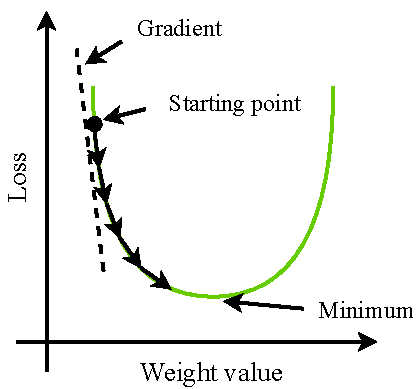
\includegraphics[width=0.5\textwidth]{diagrams/6-cnn/gradient_descent.pdf}
    \caption[Illustration of the gradient descent process]
    {Simplified illustration of the gradient descent procedure. Shown is the case for a loss
        function dependent on a single weight.}
    \label{fig:gradient_descent}
\end{figure}

Therefore, to use gradient descent, we require that the gradient of the loss function with respect
to the parameters of the network can be calculated. Doing this for each parameter at every
iteration would render neural networks impossible to train due to the vast computational
requirements. Instead, an innovative application of the chain rule, in an algorithm called
\emph{backpropagation} is used~\cite{werbos1974}. Here we follow the derivation of the four main
backpropagation equations given in Ref.~\cite{mehta2019}.

For a network containing $L$ layers, we can index the individual layers using $l=1,\dots,L$. The
weight associated with the connection between the $k$-th neuron in layer $l-1$ and the $j$-th
neuron in layer $l$ can be denoted as $w^{l}_{jk}$, with the bias of the layer $l$ neuron
correspondingly written as $b^{l}_{j}$. The activation of the $j$-th neuron in layer $l$ is then
related to the outputs from the previous layer by
\begin{equation} % PREVIOUS LAYER EQUATION %
    a^{l}_{j}=\sigma(z^{l}_{j})=\sigma\left(\sum_{k}w^{l}_{jk}a^{l-1}_{k}+b^{l}_{j}\right),
    \label{eq:feedforward}
\end{equation}
where $\sigma$ is the non-linear activation function.

The change in the loss function with respect to the linear weighted sum $z^{L}_{j}$ of the $j$-th
neuron in the last layer $L$, defines the error $\Delta^{L}_{j}$, such that
\begin{equation} % PREVIOUS LAYER EQUATION %
    \Delta^{L}_{j}=\frac{\partial E}{\partial z^{L}_{j}}.
\end{equation}
Using the chain rule and the fact that $a^{L}_{j}=\sigma(z^{L}_{j})$, the error is found to be
equivalent to
\begin{equation} % BACKPROP EQUATION 1 %
    \Delta^{L}_{j}=\frac{\partial E}{\partial a^{L}_{j}}
    \sigma '(z^{L}_{j}),
    \label{eq:backprop_1}
\end{equation}
where $\sigma '(z^{L}_{j})$ denotes the derivative of the non-linear activation function at
$z^{L}_{j}$. This (Eq.~\ref{eq:backprop_1}) is the first of the backpropagation equations.

The error $\Delta^{l}_{j}$, of the $j$-th neuron in layer $l$ can be expressed in terms of the
error in the following layer $l+1$, by using
\begin{equation} % BACKPROP EQUATION 3 %
    \begin{aligned}[b]
        \Delta^{l}_{j} &=\frac{\partial E}{\partial z^{l}_{j}}, \\
        &=\sum_{k}\frac{\partial E}{\partial z^{l+1}_{k}}
        \frac{\partial z^{l+1}_{k}}{\partial z^{l}_{j}}, \\
        &=\sum_{k}\Delta^{l+1}_{k}\frac{\partial z^{l+1}_{k}}{\partial z^{l}_{j}}, \\
        &=\left(\sum_{k}\Delta^{l+1}_{k}w^{l+1}_{kj}\right)\sigma '(z^{l}_{j}).
        \label{eq:backprop_2}
    \end{aligned}
\end{equation}
The chain rule has again been used in addition to the fact that
\begin{equation}
    z^{l+1}_{k}=\sum_{j}w^{l+1}_{kj}\sigma(z^{l}_{j})+b^{l+1}_k,
\end{equation}
to give the second of the backpropagation equations (Eq.~\ref{eq:backprop_2}).

As $\partial b^{l}_{j}/\partial z^{l}_{j}=1$, the error can also be viewed as the partial
derivative of the loss function with respect to the bias, such that
\begin{equation} % BACKPROP EQUATION 2 %
    \Delta^{l}_{j}=\frac{\partial E}{\partial z^{l}_{j}}
    =\frac{\partial E}{\partial b^{l}_{j}}\frac{\partial b^{l}_{j}}{\partial z^{l}_{j}}
    =\frac{\partial E}{\partial b^{l}_{j}},
    \label{eq:backprop_3}
\end{equation}
giving the third of the backpropagation equations (Eq.~\ref{eq:backprop_3}).

The final backpropagation equation is given by the differential of the cost function with respect
to the weight $w^{l}_{jk}$, which can be written as
\begin{equation} % BACKPROP EQUATION 4 %
    \frac{\partial E}{\partial w^{l}_{jk}}
    =\frac{\partial E}{\partial z^{l}_{j}}\frac{\partial z^{l}_{j}}{\partial w^{l}_{jk}}
    =\Delta^{l}_{j}a^{l-1}_{k}.
    \label{eq:backprop_4}
\end{equation}

The full backpropagation algorithm then proceeds as follows:
\begin{enumerate}
    \item After calculating the activations $a^{1}_{j}$ for all neurons in the input layer, use
          the feed-forward architecture of the network to calculate all the activations at every
          layer using Eq.~\ref{eq:feedforward}.
    \item Use Eq.~\ref{eq:backprop_1} to calculate the errors of the last layer neurons, requiring
          both the derivatives of the loss and activation functions.
    \item Use Eq.~\ref{eq:backprop_2} to `backpropagate' the error through the network from the
          last layer to the input layer, calculating all $\Delta^{l}_{j}$ values.
    \item Calculate the gradient of the loss function for all the weights and biases using
          Eq.~\ref{eq:backprop_3} and Eq.~\ref{eq:backprop_4}.
\end{enumerate}

A single activation finding \emph{forward pass} followed by a single error propagating
\emph{backward pass} is all that's required to calculate the gradients for all weights and biases
within the network. This incredibly efficient procedure allows for the use of gradient descent
when training neural networks.

\subsection{Convolutional neural networks} %%%%%%%%%%%%%%%%%%%%%%%%%%%%%%%%%%%%%%%%%%%%%%%%%%%%%%%
\label{sec:cnn_theory_conv} %%%%%%%%%%%%%%%%%%%%%%%%%%%%%%%%%%%%%%%%%%%%%%%%%%%%%%%%%%%%%%%%%%%%%%

The broad category of deep learning covers multiple neural network techniques spanning a range of
application fields such as computer vision, speech recognition, and natural language processing.
By stacking many layers on top of each other to form a `deep' network, these methods offer
increased problem solving capacity by allowing higher-order non-linear functions to form
throughout the network. As a direct consequence, instead of requiring hand-engineered features as
input, deep networks can learn to extract the most powerful features for a given task from raw
data. Here we outline just the specific deep learning technique used in this work; the CNN.

\subsubsection*{CNN operations} %%%%%%%%%%%%%%%%%%%%%%%%%%%%%%%%%%%%%%%%%%%%%%%%%%%%%%%%%%%%%%%%%%

At their core, CNNs make use of a mathematical operation called \emph{convolution}, which either
entirely or in part replaces the simple vector multiplication seen in the fully-connected networks
of Section.~\ref{sec:cnn_theory_basics}. This difference makes CNNs incredibly powerful for
applications with grid-like input data such as computer vision tasks.

Using standard CNN terminology, the discrete convolution between the \emph{input} $x$, and the
\emph{kernel} $w$, is given by
\begin{equation}
    f_{i}=(x*w)_{i}=\sum^{\infty}_{j=-\infty}x_{j}w_{i-j},
    \label{eq:convolution}
\end{equation}
where $f$ is commonly referred to as the \emph{feature map}. In typical applications, the input is
a two-dimensional array $X$. Therefore, both the kernel $W$, and the resulting feature map $F$,
also become two-dimensional. In this case the convolution operation becomes
\begin{equation}
    F_{i}=(X*W)_{i,j}=\sum_{m}\sum_{n}X_{i+m,j+n}W_{m,n},
    \label{eq:conv}
\end{equation}
where the infinite sum in Eq.~\ref{eq:convolution} has been replaced with a discrete sum over
two-dimensional elements. Analogous to the simple neural network weights $\vec{w}$, first
described in Eq.~\ref{eq:network}, the elements of $W_{m,n}$ are trained to minimise the loss,
with the output feature maps passed through a non-linear activation function at each layer.

To illustrate the convolution operation, Fig.~\ref{fig:conv_input} displays examples of a $4
\times 4$ input grid and a $3 \times 3$ kernel. The output feature map is generated by sliding the
kernel across both dimensions of the input grid, summing the products of all associated elements
at each step according to Eq.~\ref{eq:conv}, as shown in Fig.~\ref{fig:conv_operation}.

\begin{figure} % CONV INPUTS DIAGRAM %
    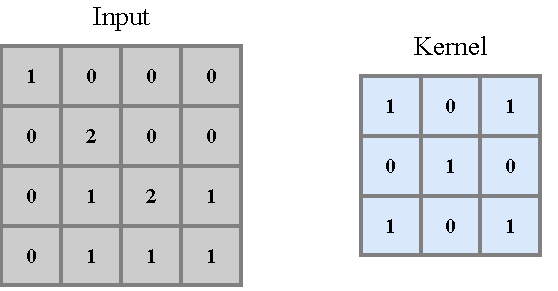
\includegraphics[width=0.7\textwidth]{diagrams/6-cnn/conv_input.pdf}
    \caption[Example of a Convolutional Neural Network input grid and kernel]
    {Example of an input grid (left) and kernel (right). The specific kernel shown is sensitive to
        x-shaped features}
    \label{fig:conv_input}
\end{figure}

\begin{figure} % CONV OPERATION DIAGRAM %
    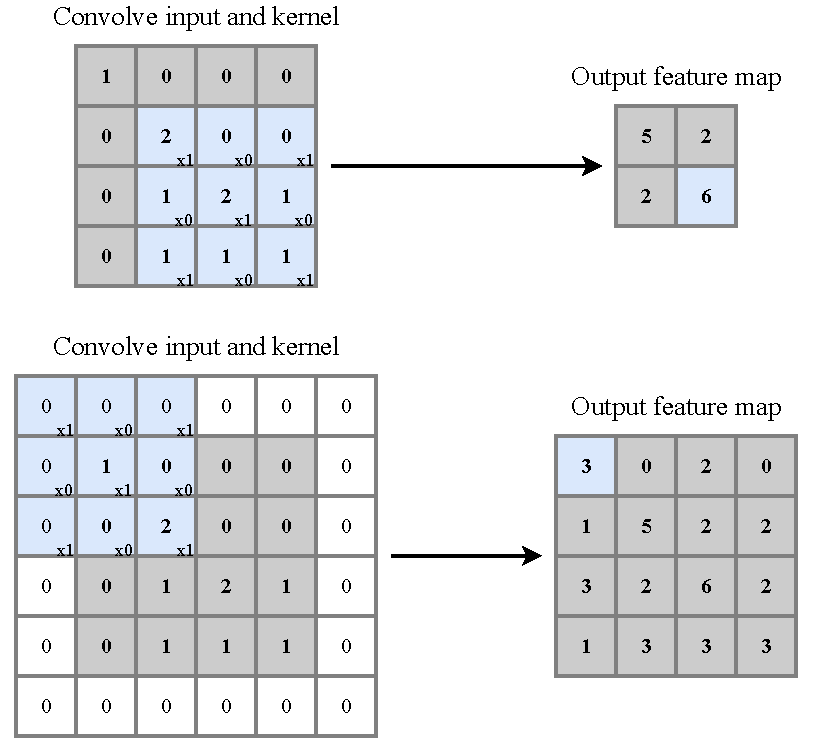
\includegraphics[width=0.8\textwidth]{diagrams/6-cnn/conv_operation.pdf}
    \caption[Example of a convolution operation]
    {Example of a $\text{stride}=1$ convolution operation involving the input grid and kernel from
        Fig.~\ref{fig:conv_input}. Both the operation for the case of \emph{valid} (top) and
        \emph{same} (bottom) padding is shown. The blue square in the top-left of the output
        feature maps indicates the output generated from the specific operation shown on the left,
        also in blue.}
    \label{fig:conv_operation}
\end{figure}

Two additional parameters impacting the feature map output size are introduced in
Fig.~\ref{fig:conv_operation}. The \emph{stride} and \emph{padding}. The stride $S$, governs how
far the kernel moves at each step while the padding $P$, decides how the input grid is padded with
zeros around its border. If $L$ is the size of the input (both height and width) and $K$ is the
kernel size, the output feature map size $O$, is given by
\begin{equation}
    O=\frac{(L-K+2P)}{S}+1.
    \label{eq:conv_size}
\end{equation}

The other essential operation used within CNNs is pooling. Pooling layers coarse-grain the spatial
information of the input to reduce the number of network parameters. \emph{Max pooling} or
\emph{average pooling} are the two common ways this is achieved. In both cases, the input is first
divided into rectangular regions, and then either the maximum or average value of the region is
returned as output, for max or average pooling respectively. Both pooling procedures are
illustrated in Fig.~\ref{fig:pooling}.

\begin{figure} % POOLING DIAGRAM %
    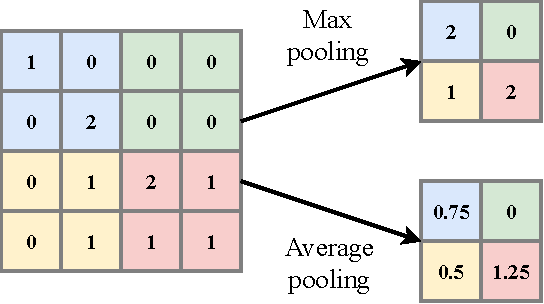
\includegraphics[width=0.7\textwidth]{diagrams/6-cnn/pooling.pdf}
    \caption[Example of pooling operation]
    {Example of both a max and average $2 \times 2$ pooling operation with $\text{stride}=2$.}
    \label{fig:pooling}
\end{figure}

Taking inspiration from how neurons behave in the visual cortex of animals~\cite{lecun2015}, small
kernels are typically used to only scan over a small patch of the input at a time. Combined with
the loss of absolute position information from pooling, a key feature of CNNs is highlighted. They
exhibit translational invariance and respect the local structure contained within the input. In
simpler terms, they do not care wherein the input image a particular feature exists, just that it
exists.

\subsubsection*{CNN architectures} %%%%%%%%%%%%%%%%%%%%%%%%%%%%%%%%%%%%%%%%%%%%%%%%%%%%%%%%%%%%%%%

In 2012 the AlexNet CNN lowered the error rate on the ubiquitous ImageNet classification
task~\cite{deng2009} from 28\% to 16\%~\cite{krizhevsky2012}. Since this breakthrough, the
standard CNN has adopted a similar architecture to AlexNet. Multiple convolutional layers are
stacked on top of each other, periodically interspersed with pooling layers. Once the output
feature map size no longer allows for additional pooling, one or more fully-connected layers are
appended before the output layer, as is illustrated in Fig.~\ref{fig:conv_diagram}.

\begin{figure} % CONV DIAGRAM %
    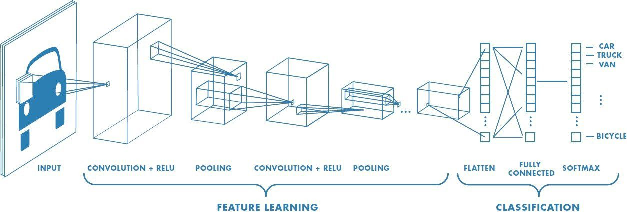
\includegraphics[width=\textwidth]{diagrams/6-cnn/conv_diagram.pdf}
    \caption[Typical Convolutional Neural Network architecture]
    {Illustration of a typical CNN architecture, containing convolutional, pooling and
        fully-connected layers before the final output layer.}
    \label{fig:conv_diagram}
\end{figure}

Led primarily by large research teams at the technology giants, improvements upon this standard
architecture have since been made. Initially, this process involved the addition of extra
convolutional layers to form deeper and deeper networks, as was done by the VGG architecture in
2014~\cite{simonyan2014}. Another approach was the introduction of the \emph{inception module}
within the GoogLeNet~\cite{szegedy2015} architecture, allowing for different feature scales to be
considered.

ResNet introduced residual connections in 2016~\cite{he2016_original, he2016_improved}. By adding
connections skipping specific layers, a larger gradient could reach the lower layers of the
network, increasing learning. Recently, the inception module and ResNet concepts have been
combined~\cite{szegedy2016}, and there has been a significant push for efficient rather than just
deeper networks~\cite{sandler2018, tan2019}. The common repeating layer patterns that form the
above networks are shown in Fig.~\ref{fig:blocks} for reference.

\begin{figure} % BLOCKS DIAGRAM %
    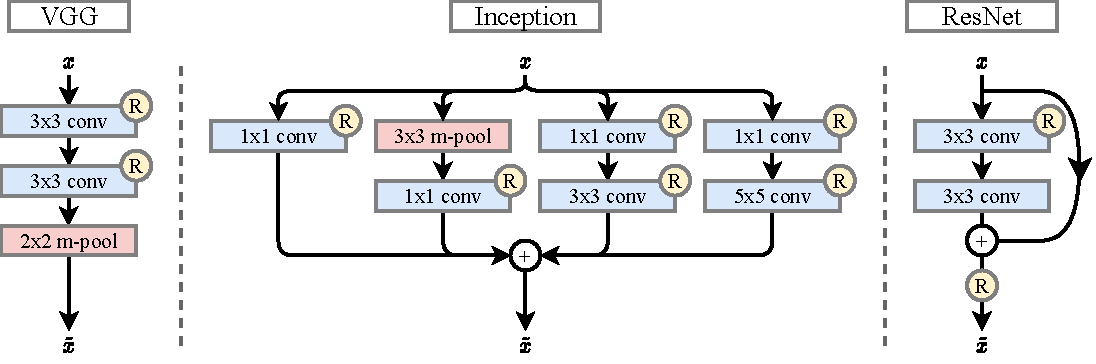
\includegraphics[width=\textwidth]{diagrams/6-cnn/blocks.pdf}
    \caption[Common Convolutional Neural Network architecture blocks]
    {Common repeating layer \emph{blocks} used within CNN architectures, taking $x$ as input and
        producing $\tilde{x}$ as output through operations whose forward pass is shown with the
        arrows. The blue and red boxes represent convolutional (conv) and max-pooling (m-pool)
        layers respectively, with the size of the operation shown. The circular yellow $R$
        indicates the use of the ReLU activation function.}
    \label{fig:blocks}
\end{figure}

\subsection{Regularisation} %%%%%%%%%%%%%%%%%%%%%%%%%%%%%%%%%%%%%%%%%%%%%%%%%%%%%%%%%%%%%%%%%%%%%%
\label{sec:cnn_theory_reg} %%%%%%%%%%%%%%%%%%%%%%%%%%%%%%%%%%%%%%%%%%%%%%%%%%%%%%%%%%%%%%%%%%%%%%%

A key challenge when training supervised machine learning models is ensuring that they can
generalise to new, previously unseen data, not within the training dataset. With networks
typically containing millions of trainable parameters, it can become effortless for them to learn
specific features and noise of the training dataset, rather than generalisable features. This
unwanted learning, called \emph{overfitting}, is ubiquitous when training CNNs. Methods used
within this work to prevent overfitting are outlined below, all of which are commonly referred to
as \emph{regularisation} techniques.

\subsubsection*{Stochastic gradient descent} %%%%%%%%%%%%%%%%%%%%%%%%%%%%%%%%%%%%%%%%%%%%%%%%%%%%%

The gradient descent update equation outlined in Eq.~\ref{eq:update_rule} updates the network
weights at each training iteration using the gradient calculated over the full dataset. This
procedure is called \emph{batch training}. It is instead much more common to calculate an
approximation to the complete gradient at each iteration using a \emph{minibatch} of the full
dataset. This is done by considering just a subset of the training data with a size commonly
referred to as the \emph{batch size} and typically equal to a power of two for computational
reasons.

This modification to standard batch training gradient descent is called \emph{stochastic gradient
    descent} as it introduces stochasticity to the training process, providing two main
    advantages. Firstly the computational speed of each iteration is significantly reduced, and
    crucially the memory requirements lowered. Secondly, the addition of minibatch specific noise
    decreases the chance that the minimisation will get stuck in a local minimum suited to
    overfitting the training dataset.

\subsubsection*{Early stopping} %%%%%%%%%%%%%%%%%%%%%%%%%%%%%%%%%%%%%%%%%%%%%%%%%%%%%%%%%%%%%%%%%%

\emph{Early stopping} is another simple regularisation procedure. During training, the training
dataset is commonly iterated over multiple times, with each iteration called an \emph{epoch}. By
evaluating the error on an independent \emph{validation} dataset at the end of each epoch, the
point at which overfitting starts to occur can be determined, as illustrated in
Fig.~\ref{fig:early_stopping}. At the determined epoch, the training is stopped to return the best
possible generalised model. In practice, it is common only to stop training after $n$ number of
epochs have passed with no validation error improvement.

\begin{figure} % EARLY STOPPING DIAGRAM %
    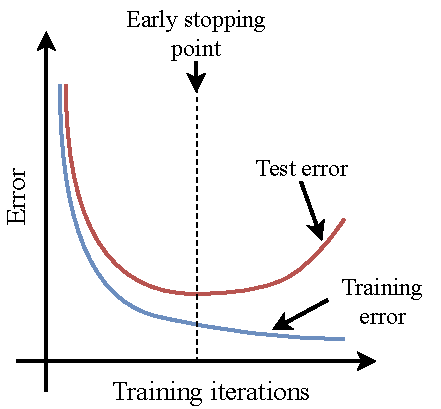
\includegraphics[width=0.5\textwidth]{diagrams/6-cnn/early_stopping.pdf}
    \caption[Illustration of the early stopping procedure]
    {Illustration of the early stopping procedure. Initially both the training and test error
        decreases, but, at some point the test error will start to increase due to overfitting, at
        this point the training is stopped.}
    \label{fig:early_stopping}
\end{figure}

\subsubsection*{Batch normalisation} %%%%%%%%%%%%%%%%%%%%%%%%%%%%%%%%%%%%%%%%%%%%%%%%%%%%%%%%%%%%%

The training of a neural network is found to work best when the inputs of each neuron are centred
on zero with respect to the bias of the neuron. This is because large input values can cause
saturation of the activation function and subsequent vanishing of the associated gradient,
reducing the ability of the network to learn. To counter this, \emph{batch normalisation}
introduces layers that standardise the inputs by using both the mean and variance of each
minibatch~\cite{ioffe2015}. This modification not only speeds up training by preventing the
vanishing of gradients, but also reduces overfitting by using the stochasticity of the minibatch.

\subsubsection*{Dropout} %%%%%%%%%%%%%%%%%%%%%%%%%%%%%%%%%%%%%%%%%%%%%%%%%%%%%%%%%%%%%%%%%%%%%%%%%

\emph{Dropout} is another simple technique to reduce overfitting~\cite{hinton2012}. At each
training iteration, each neuron has a probability $p_{d}$ to be \emph{dropped out} and ignored for
that iterations calculation. This is illustrated in Fig.~\ref{fig:dropout}. By ignoring a subset
of neurons at each iteration, it is difficult for the network to form the particularly strong
connections that are usually responsible for overfitting, leading to greater generalisation.

\begin{figure} % DROPOUT DIAGRAM %
    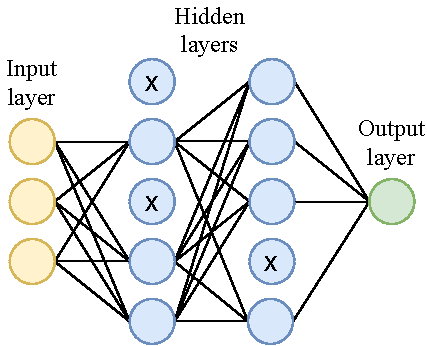
\includegraphics[width=0.6\textwidth]{diagrams/6-cnn/dropout.pdf}
    \caption[Illustration of dropout]
    {Example of dropout applied to the network shown in Fig.~\ref{fig:network}. Neurons are
        randomly \emph{dropped out} and not considered at each training step. This reduces the
        strong connections between neurons that can lead to overfitting.}
    \label{fig:dropout}
\end{figure}

\section{A baseline implementation for CHIPS} %%%%%%%%%%%%%%%%%%%%%%%%%%%%%%%%%%%%%%%%%%%%%%%%%%%%
\label{sec:cnn_baseline} %%%%%%%%%%%%%%%%%%%%%%%%%%%%%%%%%%%%%%%%%%%%%%%%%%%%%%%%%%%%%%%%%%%%%%%%%

The raw output from a water Cherenkov detector, such as those envisioned by the \chips concept, is
a simple image of each event where two channels of information are known for each PMT: the number
of collected photoelectrons, and the associated hit times. Therefore, it is a natural fit to use
CNNs developed for image-based computer vision tasks for \chips event analysis.

For this purpose, a Python-based software package named \emph{chipsnet}~\cite{chipsnet2020} has
been built. By using the high-level \emph{Application Programming Interfaces} (APIs) provided by
the Tensorflow framework (version 2.3.0)~\cite{tf2015}, a full pipeline including data
preparation, network training, and performance evaluation has been implemented. In this section,
the baseline CNN implementation built into chipsnet is outlined. The specific network
implementations described in Section.~\ref{sec:cnn_specific} share this common baseline with a few
specific differences.

\subsection{Baseline inputs} %%%%%%%%%%%%%%%%%%%%%%%%%%%%%%%%%%%%%%%%%%%%%%%%%%%%%%%%%%%%%%%%%%%%%
\label{sec:cnn_baseline_inputs} %%%%%%%%%%%%%%%%%%%%%%%%%%%%%%%%%%%%%%%%%%%%%%%%%%%%%%%%%%%%%%%%%%

The primary difficulty in the application of CNNs to \chips is determining how to map an event
captured on a cylindrical surface to a two-dimensional grid. Furthermore, this must be done in
such a way as not to distort the underlying Cherenkov emission topology which could inhibit
network learning. As a solution, this work takes inspiration and then builds upon the ideas
outlined in Ref.~\cite{theodore2016}. Simply put, an event is mapped onto a two-dimensional grid
as though it is viewed from its estimated interaction vertex position. The primary motivation
behind this is to remove any detector shape effects and to focus on the underlying event topology
and Cherenkov emission profiles.

To estimate the interaction vertex position for each event, the top-scoring seed from the seeding
procedure introduced in Section.~\ref{sec:cnn_old_reco} is used. This process, unlike the full
likelihood fit, requires no track hypothesis and typically takes under \unit{0.1}{\text{seconds}}
per event on a standard batch farm computing node. The seed estimated vertex position resolutions
for a sample of expected beam events are shown in Fig.~\ref{fig:explore_true_reco_vtx}. The $x$
component is commonly estimated closer to the downstream wall of the detector than reality,
however, as the $y$ and $z$ components perpendicular to the beam primarily drive event
distortions, the impact on event topology is small.

\begin{figure} % HOUGH VTX RES DIAGRAM %
    \includegraphics[width=\textwidth]{diagrams/7-results/explore_true_reco_vtx.pdf}
    \caption[Seeding estimated interaction vertex position resolutions]
    {Seeding estimated interaction vertex position resolution, split by component. The large
        negative tail for the $x$ component shows the tendency of the seeding procedure to
        estimate the $x$ component closer to the downstream detector wall than reality.}
    \label{fig:explore_true_reco_vtx}
\end{figure}

Using $\theta$ and $\phi$ components calculated as viewed from the estimated interaction vertex
position facing along the x-axis (downstream), hit PMTs are mapped onto a $64 \times 64$ grid.
This procedure is used to generate two event \emph{maps}. Firstly, a \emph{hit-charge} map where
each grid bin is given by the total collected photoelectrons from all PMTs mapped to that bin.
Secondly, a \emph{hit-time} map where each grid bin is given by the first hit time (in
nanoseconds) across all PMTs mapped to that bin. Each hit-time map is further corrected so that
the first hit time across all bins lies at zero. Note that within this work veto PMTs are ignored
for simplicity.

By design, the Hough transform within the seeding procedure uses the estimated interaction vertex
position to generate the transform space. Therefore, by re-binning the transform space to a $64
\times 64$ grid a third \emph{hough-height} map is generated for each event. This event map aims
to provide a complementary but different representation of the event where Cherenkov rings are
instead represented as peaks, allowing for additional discriminating features to be learnt.

All three event maps: hit-charge, hit-time, and hough-height are down-sampled (from 32-bit floats)
using 8-bit encoding. The encoding not only significantly reduces storage requirements but also
dramatically increases the speed with which data can be loaded during training (which turns out to
be the primary training bottleneck). For each map type, a range over which to encode from zero up
to a \emph{cap-point} is chosen to minimise the number of bin values that are capped at the
maximum encoded value of 255. Table.~\ref{tab:encoding} shows the cap-points and the associated
percentage of bin values capped for each map type, while Fig.~\ref{fig:explore_8_bit_range} shows
the distribution of bin values for each event map across the encoded range.

\begin{table}
    \begin{tabular}{lrr}
        Event map    & Cap-point & Capped percentage \\
        \midrule
        hit-charge   & 25 p.e    & 0.10\%            \\
        hit-time     & 120 ns    & 0.15\%            \\
        hough-height & 3500 p.e  & 0.23\%            \\
    \end{tabular}
    \caption[Table of input event map 8-bit cap-points and percentages]
    {Table showing the input event map cap-points (maximum value of the encoding range) and the
        associated percentage of bin values that are capped at the maximum 8-bit value of 255 as a
        consequence. The cap-points are specifically chosen so that the capped percentage is
        approximately 0.1\%, keeping any information loss low.}
    \label{tab:encoding}
\end{table}

\begin{figure} % 8-BIT DIAGRAM %
    \includegraphics[width=0.7\textwidth]{diagrams/7-results/explore_8_bit_range.pdf}
    \caption[Event map encoded 8-bit distributions]
    {The distribution of encoded 8-bit values for the hit-charge, hit-time and hough-height event
        maps. Note the maximum (capped) bin at an 8-bit value of 255.}
    \label{fig:explore_8_bit_range}
\end{figure}

Event maps for example events generated using the above procedure are shown in
Fig.~\ref{fig:explore_nuel_ccres_event} for a CC resonant $\nu_{e}$ event, in
Fig.~\ref{fig:explore_numu_ccdis_event} for a CC DIS $\nu_{\mu}$ event, in
Fig.~\ref{fig:explore_nuel_ncdis_event} for a NC DIS event, and in
Fig.~\ref{fig:explore_cosmic_event} for a cosmic muon event.

\begin{figure} % NUEL EVENT DIAGRAM %
    \includegraphics[width=\textwidth]{diagrams/7-results/explore_nuel_ccres_event.pdf}
    \caption[Example of a CC resonant $\nu_{e}$ event]
    {Three map representation of a CC resonant $\nu_{e}$ event. Initiated by a $\nu_{e}$ of energy
        \unit{3.3}{\GeV} the final state particles above the Cherenkov threshold include a $e^{-}$
        of energy \unit{2.8}{\GeV} and a \unit{0.3}{\GeV} $\pi^{0}$.}
    \label{fig:explore_nuel_ccres_event}
\end{figure}

\begin{figure} % NUMU EVENT DIAGRAM %
    \includegraphics[width=\textwidth]{diagrams/7-results/explore_numu_ccdis_event.pdf}
    \caption[Example of a CC DIS $\nu_{\mu}$ event]
    {Three map representation of a CC DIS $\nu_{\mu}$ event. Initiated by a $\nu_{\mu}$ of energy
        \unit{3.5}{\GeV} the final state particles above the Cherenkov threshold include a
        $\mu^{-}$ of energy \unit{1.9}{\GeV}, a proton of energy\unit{2.0}{\GeV}, and a
        \unit{0.2}{\GeV} $\pi^{-}$.}
    \label{fig:explore_numu_ccdis_event}
\end{figure}

\begin{figure} % NC EVENT DIAGRAM %
    \includegraphics[width=\textwidth]{diagrams/7-results/explore_nuel_ncdis_event.pdf}
    \caption[Example of a NC DIS event]
    {Three map representation of a NC DIS event. Initiated by a $\nu_{e}$ of energy
        \unit{9.3}{GeV} the final state particles above the Cherenkov threshold include a proton
        of energy \unit{2.6}{\GeV} and a \unit{2.5}{\GeV} $\pi^{-}$.}
    \label{fig:explore_nuel_ncdis_event}
\end{figure}

\begin{figure} % COSMIC MUON EVENT DIAGRAM %
    \includegraphics[width=\textwidth]{diagrams/7-results/explore_cosmic_event.pdf}
    \caption[Example of a cosmic muon event]
    {Three channel representation of a cosmic muon event, containing a $\mu^{-}$ of energy
        \unit{2.9}{\GeV}.}
    \label{fig:explore_cosmic_event}
\end{figure}

\subsection{Baseline architecture} %%%%%%%%%%%%%%%%%%%%%%%%%%%%%%%%%%%%%%%%%%%%%%%%%%%%%%%%%%%%%%%
\label{sec:cnn_baseline_arch} %%%%%%%%%%%%%%%%%%%%%%%%%%%%%%%%%%%%%%%%%%%%%%%%%%%%%%%%%%%%%%%%%%%%

An illustrative diagram of the baseline chipsnet architecture is shown in Fig.~\ref{fig:chipsnet}.
Based on the VGG network previously mentioned in Section.~\ref{sec:cnn_previous} and detailed in
Ref.~\cite{simonyan2014} there are a few key differences from the literature defined network.

\begin{figure} % CHIPSNET DIAGRAM %
    \includegraphics[width=0.7\textwidth]{diagrams/6-cnn/chipsnet.pdf}
    \caption[Illustrative diagram of the baseline chipsnet architecture]
    {Illustrative diagram of the baseline chipsnet architecture. The three input event maps are
        separately passed through two VGG blocks each before their outputs are combined and passed
        through a further three VGG blocks together. The flattened VGG blocks outputs are then
        concatenated with five seed parameters (seed pars) and passed through two fully-connected
        (FC) layers of 512 neurons each before the output layer. Both the number of convolutional
        units and kernels is shown for each block. The detailed VGG block structure is shown
        within the grey box. The circular yellow $R$ and $Bn$ indicate the use of the ReLU
        activation function and batch normalisation, respectively.}
    \label{fig:chipsnet}
\end{figure}

\begin{itemize}
    \item Each of the three event maps: hit-charge, hit-time, and hough-height are initially fed
          into three separate branches. Each branch contains two VGG blocks with two convolutional
          layers each (four convolutional layers in total). The outputs from each branch are
          merged using a concatenation layer before being fed to the rest of the network. This
          configuration allows for event map specific features to be learnt independently before
          combined features are learnt by the rest of the network.

    \item Batch normalisation as described in Section.~\ref{sec:cnn_theory_reg} is included before
          the activation (ReLU) function for every convolutional layer.

    \item Squeeze-and-excitation units, as detailed in Ref.~\cite{hu2018} are included after the
          max-pooling operation in all VGG blocks. These units introduce extra parameters to model
          the interdependencies between output feature maps, allowing the network to learn how to
          weight each feature map effectively.

    \item Dropout is included at the end of each VGG block as well as after the final
          fully-connected layer. Instead of dropping individual kernel elements, the dropout
          within the VGG blocks drops entire kernels at each training iteration, this is commonly
          called \emph{two-dimensional spatial dropout}. The dropout after the fully-connected
          layers is standard, in that it drops out individual fully-connected neurons.

    \item Five output parameters from the seeding process (seed pars) are concatenated with the
          flattened layer before the fully-connected layers. Included are the three components of
          the estimated interaction vertex position ($s_{x},s_{y}, s_{z}$), and the two components
          of the estimated track direction ($s_{\theta},s_{\phi}$). These parameters provide the
          network with spatial context as to where in the detector the input event maps have been
          generated and the dominant direction of PMT activity.
\end{itemize}

The chipsnet baseline architecture is implemented using the Keras~\cite{chollet2015} API built
into Tensorflow. Keras allows for predefined common layers such as a two-dimensional convolution
or a max-pooling layer to be easily structured into a full network definition.

\subsection{Baseline outputs} %%%%%%%%%%%%%%%%%%%%%%%%%%%%%%%%%%%%%%%%%%%%%%%%%%%%%%%%%%%%%%%%%%%%
\label{sec:cnn_baseline_outputs} %%%%%%%%%%%%%%%%%%%%%%%%%%%%%%%%%%%%%%%%%%%%%%%%%%%%%%%%%%%%%%%%%

Many CNN applications are found to benefit from learning multiple tasks at the same time. This is
believed to be the case as training with multiple tasks tends to return a network with an improved
generalised representation of the inputs, with features learnt for one task improving the
performance of another. Additionally, multiple tasks work to regularise any one output from
overfitting. Commonly named \emph{multi-task} learning, this methodology is used extensively in
this work.

To train a network with multiple tasks (outputs), a loss function $E_{tot}$ must be defined to
combine the individual loss functions for each task $E_{i}$. The simplest way to do this is via a
linear weighted sum, such that
\begin{equation}
    E_{tot} = \sum_{i=1}^{i=N}w_{i}E_{i},
    \label{eq:multi_simple}
\end{equation}
where $N$ is the number of tasks and $w_{i}$ are the associated weights. In this work this is
referred to as the \emph{simple} multi-task loss.

However, the final network performance can strongly depend on the relative weighting between loss
functions, especially when the values returned by each differ by many order of magnitude (common
when combining regression and classification tasks). Therefore, finding the optimal $w_{i}$
weights can be both difficult and time-consuming. Another approach outlined in
Ref.~\cite{kendall2018} remedies this problem by learning the optimal weighting between loss
functions. This is done by introducing an additional trainable parameter $\sigma_{i}$, for each
loss function, such that
\begin{equation}
    E_{tot}= \sum_{i=1}^{i=N}\frac{1}{2\sigma_{i}^2}E_{i}+ \log\sigma_{i}.
    \label{eq:multi_learnt}
\end{equation}
In this work we refer to this as the \emph{learnt} multi-task loss.

The specific number and nature of outputs for the specific networks are detailed in
Section.~\ref{sec:cnn_specific}. Although physically motivated to some degree, the exact set of
tasks and the loss combination technique used is mainly driven by extensive trial-and-error. The
chipsnet software is specifically designed to enable this process by making it easy to configure
the network outputs via a simple configuration file.

\subsection{Baseline training} %%%%%%%%%%%%%%%%%%%%%%%%%%%%%%%%%%%%%%%%%%%%%%%%%%%%%%%%%%%%%%%%%%%
\label{sec:cnn_baseline_training} %%%%%%%%%%%%%%%%%%%%%%%%%%%%%%%%%%%%%%%%%%%%%%%%%%%%%%%%%%%%%%%%

All networks are trained on an 18 core CPU (36 thread) machine equipped with four NVIDIA GeForce
RTX 2080 graphics processing units (GPUs). The Tensorflow dataset API is used to create an
efficient input data pipeline where data is loaded on-the-fly at training time. This procedure
ensures all CPU threads are utilised loading, decoding, and preprocessing data for the primary GPU
based network calculations before being needed, maximising computational efficiency.

During preprocessing, all 8-bit input event map values are converted to 32-bit float values
bounded between zero and one. Furthermore, a random factor scaling is applied to each map bin.
Generated from a normal distribution centred on one with a standard deviation of $\sigma_{r}$, by
fluctuating the bin values the network is forced to focus less on the absolute bin values and more
on the underlying event topology. Not only does this process provide valuable regularisation to
reduce overfitting, but also makes the trained networks robust to small changes within the input
(explored within Section.~\ref{sec:results_robust}).

A minibatch training strategy of minibatch size of $n_{b}$, using the Adam
optimiser~\cite{kingma2014} ($\beta_{1}=0.9$, $\beta_{2}=0.999$, and $\epsilon = 1e-7$) is used.
The exact training sample size and composition for each specific network are given in
Section.~\ref{sec:cnn_specific}, but for all networks a 95\% training to 5\% validation data split
is employed across the full training sample. Consequently, early stopping is used. The learning
rate for each epoch $\eta_{e}$ is set to decrease throughout training according to
\begin{equation}
    \eta_{e}=\frac{\eta_{0}}{1+c_{d}(e-1)},
\end{equation}
where $\eta_{0}$ is the initial learning rate, $e$ is the epoch number (starting at one), and
$c_{d}$ is the learning rate decay coefficient.

Therefore, when training each network there is a list of tunable \emph{hyperparameters}. All are
optimised specifically for each network using the SHERPA hyperparameter tuning
framework~\cite{hertel2020}. To maximise performance, random configurations are tested within
SHERPA across a specific range or selection of choices for each hyperparameter, with:
\begin{itemize}
    \item the \textbf{initial learning rate $\eta_{0}$}, in a range from $0.00005$ to $0.001$;
    \item the \textbf{learning rate decay coefficient $c_{d}$}, in a range from $0.2$ to $0.8$;
    \item the \textbf{dropout probability $p_{d}$}, in a range from $0.0$ to $0.5$;
    \item the \textbf{random scaling size $\sigma_{r}$}, in a range from $0.0$ to $0.1$;
    \item the \textbf{minibatch size $n_{b}$}, choosing from either $32$, $64$, $128$, or $256$;
    and
    \item the \textbf{multi-task loss combination strategy}, choosing from either simple or
    learnt.
\end{itemize}

\section{Specific implementations for CHIPS} %%%%%%%%%%%%%%%%%%%%%%%%%%%%%%%%%%%%%%%%%%%%%%%%%%%%%
\label{sec:cnn_specific} %%%%%%%%%%%%%%%%%%%%%%%%%%%%%%%%%%%%%%%%%%%%%%%%%%%%%%%%%%%%%%%%%%%%%%%%%

The specific CNN implementations for cosmic rejection, beam classification, and energy estimation
are outlined below. It is important to note that the exact configuration of networks outlined here
is the result of extensive testing designed to maximise the selection of a pure and efficient
sample of CC $\nu_{e}$ beam events whose neutrino energy can also be accurately determined.

As an example of an alternative implementation, if cosmic rejection and beam classification are
combined into a single network, both objectives see a reduction in performance. The same is also
true if either cosmic rejection or beam classification is combined with neutrino energy
estimation. However, specific secondary outputs such as counting the number of primary particles
in conjunction with beam classification are seen to improve performance. It is clear, therefore,
that the multi-task approach only works for tasks that require a similar learnt representation of
the inputs. Put simply; the tasks must be similar.

\subsection{Cosmic rejection} %%%%%%%%%%%%%%%%%%%%%%%%%%%%%%%%%%%%%%%%%%%%%%%%%%%%%%%%%%%%%%%%%%%%
\label{sec:cnn_specific_cosmic} %%%%%%%%%%%%%%%%%%%%%%%%%%%%%%%%%%%%%%%%%%%%%%%%%%%%%%%%%%%%%%%%%%

The cosmic rejection network aims to prevent the vast cosmic muon background from contaminating
the final selected sample of beam events. Therefore, the primary task is a simple binary
classification between beam and cosmic events. Additionally, training the network to also separate
events where the primary charged lepton escapes the detector volume or not, is found to improve
cosmic rejection performance. As a large proportion of cosmic muons are relatively high in energy
and, therefore, escape the detector in this fashion, there is motivation as to why this additional
task is helpful.

The network is trained on a sample of 3.15 million simulated events produced using the detector
simulation and event generation methods outlined in Section.~\ref{sec:chips_monte_carlo}. Roughly
$1/3^{rd}$ are $\nu_{\mu}$ beam events, $1/3^{rd}$ $\nu_{e}$ beam events, and $1/3^{rd}$ cosmic
muon events, the counts of which are shown in Fig.~\ref{fig:cosmic_training_sample}. All beam
events (both $\nu_{\mu}$ and $\nu_{e}$) are generated using the expected \chipsfive $\nu_{\mu}$
energy spectrum to closely mimic the dominant $\nu_{\mu}$ beam component and appeared $\nu_{e}$
signal. Every event in the sample is used for training with no preselection, as this is found to
be the best for cosmic rejection performance.

\begin{figure} % COSMIC TRAINING SAMPLE DIAGRAM %
    \includegraphics[width=0.7\textwidth]{diagrams/7-results/explore_cosmic_training_sample.pdf}
    \caption[Number of training events per category for the cosmic rejection network]
    {Number of training events per category for the cosmic rejection network. All beam event
        interaction types are shown, however, all are classed as beam events (blue) in training
        against cosmic events (red).}
    \label{fig:cosmic_training_sample}
\end{figure}

There are two outputs to the cosmic rejection network:
\begin{enumerate}
    \item \textbf{Cosmic score (1 classification neuron):} Returns a score between zero and one
          corresponding to whether the event is beam or cosmic like. The binary cross-entropy loss
          function in Eq.~\ref{eq:binary_cross_entropy} is used for training with a simple
          multi-task weight of $1$.
    \item \textbf{Escapes score (1 classification neuron):} Returns a score between zero and one
          corresponding to whether the charged lepton in an event is contained or escapes the
          detector. The binary cross-entropy loss function in Eq.~\ref{eq:binary_cross_entropy} is
          used for training with a simple multi-task weight of $1$. NC beam events without a
          charged lepton are masked (do not contribute to the loss) during training for this
          output.
\end{enumerate}

The network is allowed to train for up to 30 epochs using the SHERPA optimised hyperparameters:
$\eta_{0}=0.00005$, $c_{d}=0.7$, $p_{d}=0.1$, $\sigma_{r}=0.02$, and $n_{b}=128$, with a simple
multi-task loss combination as given in Eq.~\ref{eq:multi_simple}. Typically, only 6 epochs are
required to reach the maximum validation sample \emph{cosmic score} accuracy, with early stopping
halting training after 11 epochs (taking 15 hours), as can be seen in
Fig.~\ref{fig:final_cosmic_history}.

\begin{figure} % COSMIC HISTORY DIAGRAM %
    \includegraphics[width=0.7\textwidth]{diagrams/7-results/final_cosmic_history.pdf}
    \caption[Loss and accuracy throughout training for the cosmic rejection network]
    {Total loss and \emph{cosmic score} accuracy for both the training sample (solid) and
        validation sample (dashed) throughout training for the cosmic rejection network. The final
        network weights are taken at epoch 6 as shown by the vertical black line.}
    \label{fig:final_cosmic_history}
\end{figure}

\subsection{Beam classification}%%%%%%%%%%%%%%%%%%%%%%%%%%%%%%%%%%%%%%%%%%%%%%%%%%%%%%%%%%%%%%%%%%
\label{sec:cnn_specific_beam} %%%%%%%%%%%%%%%%%%%%%%%%%%%%%%%%%%%%%%%%%%%%%%%%%%%%%%%%%%%%%%%%%%%%

The beam classification network aims to separate beam events by their neutrino and interaction
type to primarily select a pure and efficient sample of appeared $\nu_{e}$ events, but also a
sample of survived CC $\nu_{\mu}$ events. Therefore, the principal task is a categorical
classification between CC $\nu_{e}$, CC $\nu_{\mu}$, and NC events. No attempt is made to separate
the appeared CC $\nu_{e}$ and intrinsic beam CC $\nu_{e}$ components as they are impossible to
tell apart, except for their distribution in neutrino energy.

Similar to the implementation used by DUNE~\cite{collaboration2020}, alongside the core
classification additional classification and particle counting tasks outlined below are included
to improve performance. Note that the particle counting tasks are not used in this work for
anything but increasing the primary classification performance. Future work, however, could
exploit any ability to separate exclusive final states, deduced from these particle counts, to
reduce both energy resolution and systematic errors. As an example of a method already in use,
\nova use their ability to accurately determine the hadronic energy of an event to split their CC
$\nu_{\mu}$ sample into populations of different energy resolution. Each population can then be
treated separately in the analysis before being combined, increasing overall
performance~\cite{acero2018}.

The network is trained on a sample of 1.67 million simulated events produced using the detector
simulation and event generation methods outlined in Section.~\ref{sec:chips_monte_carlo}. Roughly
half are $\nu_{\mu}$ beam events, with the other half being $\nu_{e}$ beam events, as shown in
Fig.~\ref{fig:beam_training_sample}. All events (both $\nu_{\mu}$ and $\nu_{e}$) are generated
using the expected \chipsfive $\nu_{\mu}$ energy spectrum to closely mimic the dominant
$\nu_{\mu}$ beam component and appeared $\nu_{e}$ signal. All events are used for training with no
preselection as this is found to be the best for beam classification performance, especially NC
rejection.

\begin{figure} % BEAM TRAINING SAMPLE DIAGRAM %
    \includegraphics[width=0.7\textwidth]{diagrams/7-results/explore_beam_training_sample.pdf}
    \caption[Number of training events per category for the beam classification network]
    {Number of training events per category for the beam classification network. All beam event
        interaction types are shown.}
    \label{fig:beam_training_sample}
\end{figure}

There are nine outputs to the beam classification network:
\begin{enumerate}
    \item \textbf{Combined category (3 classification neurons):} Returns a classification
          probability score between zero and one for each of CC $\nu_{e}$, CC $\nu_{\mu}$, and NC
          (summing to one). The categorical cross-entropy loss function in
          Eq.~\ref{eq:categorical_cross_entropy} is used for training with a simple multi-task
          weight of $1$.
    \item \textbf{CC category (6 classification neurons):} Returns a classification probability
          score between zero and one for each of CC-QEL, CC-Res, CC-DIS, CC-Coh, CC-MEC and
          CC-other (summing to one). The categorical cross-entropy loss function in
          Eq.~\ref{eq:categorical_cross_entropy} is used for training with a simple multi-task
          weight of $1$. NC events are masked (do not contribute to the loss) during training for
          this output.
    \item \textbf{NC category (4 classification neurons):} Returns a classification probability
          score between zero and one for each of NC-Res, NC-DIS, NC-Coh and NC-other (summing to
          one). The categorical cross-entropy loss function in
          Eq.~\ref{eq:categorical_cross_entropy} is used for training with a simple multi-task
          weight of $1$. CC events are masked (do not contribute to the loss) during training for
          this output.
    \item \textbf{Electron count (4 classification neurons):} Returns a classification probability
          score between zero and one for each of 0, 1, 2, and 3+ electrons in the final state
          (summing to one). The categorical cross-entropy loss function in
          Eq.~\ref{eq:categorical_cross_entropy} is used for training with a simple multi-task
          weight of $1$.
    \item \textbf{Muon count (4 classification neurons):} Returns a classification probability
          score between zero and one for each of 0, 1, 2, and 3+ muons in the final state (summing
          to one). The categorical cross-entropy loss function in
          Eq.~\ref{eq:categorical_cross_entropy} is used for training with a simple multi-task
          weight of $1$.
    \item \textbf{Proton count (4 classification neurons):} Returns a classification probability
          score between zero and one for each of 0, 1, 2, and 3+ protons in the final state
          (summing to one). The categorical cross-entropy loss function in
          Eq.~\ref{eq:categorical_cross_entropy} is used for training with a simple multi-task
          weight of $1$.
    \item \textbf{$\pi^{\pm}$ count (4 classification neurons):} Returns a classification
          probability score between zero and one for each of 0, 1, 2, and 3+ charged pions in the
          final state (summing to one). The categorical cross-entropy loss function in
          Eq.~\ref{eq:categorical_cross_entropy} is used for training with a simple multi-task
          weight of $1$.
    \item \textbf{$\pi^{0}$ count (4 classification neurons):} Returns a classification
          probability score between zero and one for each of 0, 1, 2, and 3+ neutral pions in the
          final state (summing to one). The categorical cross-entropy loss function in
          Eq.~\ref{eq:categorical_cross_entropy} is used for training with a simple multi-task
          weight of $1$.
    \item \textbf{Photon count (4 classification neurons):} Returns a classification probability
          score between zero and one for each of 0, 1, 2, and 3+ photons in the final state
          (summing to one). The categorical cross-entropy loss function in
          Eq.~\ref{eq:categorical_cross_entropy} is used for training with a simple multi-task
          weight of $1$.
\end{enumerate}

The network is allowed to train for up to 30 epochs using the SHERPA optimised hyperparameters:
$\eta_{0}=0.0002$, $c_{d}=0.5$, $p_{d}=0.1$, $\sigma_{r}=0.02$, and $n_{b}=128$, with a simple
multi-task loss combination as given in Eq.~\ref{eq:multi_simple}. Typically, only 7 epochs are
required to reach the maximum validation sample \emph{combined category} accuracy, with early
stopping halting training after 12 epochs (taking 15 hours), as can be seen in
Fig.~\ref{fig:final_beam_history}.

\begin{figure} % BEAM HISTORY DIAGRAM %
    \includegraphics[width=0.7\textwidth]{diagrams/7-results/final_beam_history.pdf}
    \caption[Loss and accuracy throughout training for the beam classification network]
    {Total loss and \emph{combined category} accuracy for both the training sample (solid) and
        validation sample (dashed) throughout training for the beam classification network. The
        final network weights are taken at epoch 7 as shown by the vertical black line.}
    \label{fig:final_beam_history}
\end{figure}

\subsection{Energy estimation} %%%%%%%%%%%%%%%%%%%%%%%%%%%%%%%%%%%%%%%%%%%%%%%%%%%%%%%%%%%%%%%%%%%
\label{sec:cnn_specific_energy} %%%%%%%%%%%%%%%%%%%%%%%%%%%%%%%%%%%%%%%%%%%%%%%%%%%%%%%%%%%%%%%%%%

Accurate neutrino energy estimation is accomplished using multiple networks trained on separate
samples of $\nu_{e}$ and $\nu_{\mu}$ events across multiple CC interaction types. It is found that
separation such as this results in greater performance than if a single energy estimation network
or even separate $\nu_{e}$ and $\nu_{\mu}$ networks are trained. This is expected as a single set
of network weights is unlikely to be able to capture the specific topological features that
contribute to the energy for all types of event.

Alongside the primary neutrino energy regression task, additionally learning the primary charged
lepton energy and the interaction vertex position and time is found to improve performance.
Although this improvement is relatively small for neutrino energy estimation, it dramatically
improves primary charged lepton energy estimation when compared to being predicted alone. With two
energy tasks, the network is encouraged to learn how the primary charged lepton and neutrino
energies are related. As the interaction vertex position within the detector and hence distance
from the instrumented wall can impact the number of deposited photoelectrons, there is motivation
as to why these additional tasks are also helpful.

Separate networks are trained for each of CC-QEL (and CC-MEC), CC-Res, and CC-DIS for both
$\nu_{e}$ and $\nu_{\mu}$ events (8 in total) using 250000 corresponding simulated events each.
All events (both $\nu_{\mu}$ and $\nu_{e}$) are produced using the detector simulation and event
generation methods outlined in Section.~\ref{sec:chips_monte_carlo}. The expected \chipsfive
$\nu_{\mu}$ energy spectrum is used to generate all events to closely mimic the dominant
$\nu_{\mu}$ beam component and appeared $\nu_{e}$ signal. Only events for which the primary
charged lepton is fully contained within the detector volume are used for training, with no
additional preselection applied. Note that CC-QEL and CC-MEC energy estimation is combined into a
single network as both have incredibly similar final state topologies (a single charged lepton).

There are six outputs to each of the energy estimation networks:
\begin{enumerate}
    \item \textbf{Neutrino energy (1 regression neuron):} Returns the estimated neutrino energy.
          The mean-squared error loss function in Eq.~\ref{eq:mse} is used for training.
    \item \textbf{Charged lepton energy (1 regression neuron):} Returns the estimated primary
          charged lepton energy. The mean-squared error loss function in Eq.~\ref{eq:mse} is used
          for training.
    \item \textbf{Interaction vertex x-position (1 regression neuron):} Returns the estimated
          interaction vertex x-position. The mean-squared error loss function in Eq.~\ref{eq:mse}
          is used for training.
    \item \textbf{Interaction vertex y-position (1 regression neuron):} Returns the estimated
          interaction vertex y-position. The mean-squared error loss function in Eq.~\ref{eq:mse}
          is used for training.
    \item \textbf{Interaction vertex z-position (1 regression neuron):} Returns the estimated
          interaction vertex z-position. The mean-squared error loss function in Eq.~\ref{eq:mse}
          is used for training.
    \item \textbf{Interaction time (1 regression neuron):} Returns the estimated interaction time
          relative to the first PMT hit for each event. The mean-squared error loss function in
          Eq.~\ref{eq:mse} is used for training.
\end{enumerate}

Each network is allowed to train for up to 30 epochs using the SHERPA optimised hyperparameters:
$\eta_{0}=0.0002$, $c_{d}=0.5$, $p_{d}=0.1$, $\sigma_{r}=0.0$, and $n_{b}=128$, with a learnt
multi-task loss combination as given in Eq.~\ref{eq:multi_learnt}. Early stopping typically halts
training after approximately 20 epochs (taking 2 hours). An example of how an energy estimation
networks training typically proceeds is given in Fig.~\ref{fig:final_energy_history}.

\begin{figure} % ENERGY HISTORY DIAGRAM %
    \includegraphics[width=0.7\textwidth]{diagrams/7-results/final_energy_history.pdf}
    \caption[Loss and mean absolute error throughout training for the energy estimation network]
    {Total loss and \emph{neutrino energy} mean absolute error for both the training dataset
        (solid) and validation dataset (dashed) throughout training for the energy estimation
        network trained on CC-QEL and CC-MEC $\nu_{e}$ events. The final network weights are taken
        at epoch 16 as shown by the vertical black line.}
    \label{fig:final_energy_history}
\end{figure}
    \chapter{Network evaluation} %%%%%%%%%%%%%%%%%%%%%%%%%%%%%%%%%%%%%%%%%%%%%%%%%%%%%%%%%%%%%%%%%%%%%
\label{chap:results} %%%%%%%%%%%%%%%%%%%%%%%%%%%%%%%%%%%%%%%%%%%%%%%%%%%%%%%%%%%%%%%%%%%%%%%%%%%%%

This chapter provides a comprehensive evaluation of how the new CNN approach behaves. Four
categories of understanding are explored (each a section of this chapter):
\begin{enumerate}
    \item determining the beam selection and energy estimation performance;
    \item explaining the inner workings of the trained networks;
    \item studying how robust the network outputs are to changes in the input; and
    \item exploring alternative implementations to see which factors drive performance.
\end{enumerate}

Beforehand, a hugely impactful advantage of the CNN approach must be highlighted. Although the
time taken to train the CNNs in this work is approximately two days, once trained the time
required to calculate all network outputs (inference time) for a single event is on the order of
\unit{2}{\text{ms}}. When combined with event seeding and event map generation, the total time
taken to fully reconstruct and classify a raw event is less than \unit{0.1}{\text{seconds}}.
Compared to the $\sim$\unit{15}{\text{minutes}} required for each event using the standard
reconstruction and classification methods (with multiple hypotheses), the difference is stark.

Armed with this incredible speed, the time taken to fully process a large dataset containing
millions of events becomes a matter of hours, compared to the many weeks typically required. This
change has far-reaching implications for how physics analysis is conducted. By removing the
processing bottleneck, larger datasets can be used without worry, new techniques can be tested
quickly, and overall analysis turnover is increased.

\section{Performance} %%%%%%%%%%%%%%%%%%%%%%%%%%%%%%%%%%%%%%%%%%%%%%%%%%%%%%%%%%%%%%%%%%%%%%%%%%%%
\label{sec:results_eval} %%%%%%%%%%%%%%%%%%%%%%%%%%%%%%%%%%%%%%%%%%%%%%%%%%%%%%%%%%%%%%%%%%%%%%%%%

Here the performance of the CNN approach is presented and compared to that achieved by the
standard \chips methods as well as comparable experiments. Primarily this focuses on the principle
aim of selecting an efficient and pure appeared CC $\nu_{e}$ signal sample with accurate neutrino
energy estimation. However, the survived CC $\nu_{\mu}$ selection is also presented for
completeness.

\subsection{Evaluation sample and preselection} %%%%%%%%%%%%%%%%%%%%%%%%%%%%%%%%%%%%%%%%%%%%%%%%%%
\label{sec:results_eval_sample} %%%%%%%%%%%%%%%%%%%%%%%%%%%%%%%%%%%%%%%%%%%%%%%%%%%%%%%%%%%%%%%%%%

An independent sample of events is used to evaluate the combined performance of the trained CNNs.
The evaluation sample consists of 400000 beam and 350000 cosmic muon events produced in the same
way as the training and validation events, using the detector simulation and event generation
methods outlined in Section.~\ref{sec:chips_monte_carlo}. The beam events include the expected
$\nu_{\mu}$, $\bar{\nu}_{\mu}$, $\nu_{e}$ and $\bar{\nu}_{e}$ components of the beam as well as
events generated to mimic the appeared (sometimes referred to as \emph{App}) $\nu_{e}$ component.
Only the neutrino mode (forward horn current) of NuMI beam operation is considered here. During
evaluation, the intrinsic neutrino and antineutrino components of the beam are considered the same
for simplicity.

All evaluation events are weighted to match the expected spectrum at the \chipsfive detector using
the unoscillated flux, cross-sections, and oscillation probabilities (including the MSW effect).
Additional weighting also scales the sample to match data taking in the NuMI beam for a single
year, corresponding to $6\times 10^{20}$ protons on target (POT). Cosmic muon events are weighted
according to the \unit{11.8}{\text{kHz}} expected \chipsfive rate outlined in
Section.~\ref{sec:chips_monte_carlo_cosmic}. The final weighted spectrum of events is shown in
Fig.~\ref{fig:explore_osc_fluxes} with the combination of underlying beam neutrino interaction
types shown in Fig.~\ref{fig:explore_stacked_int_types}.

\begin{figure} % OSC FLUXES DIAGRAM %
    \includegraphics[width=0.7\textwidth]{diagrams/7-results/explore_osc_fluxes.pdf}
    \caption[Weighted spectrum of evaluation sample events]
    {Weighted spectrum of events contained within the evaluation sample. The weighting is designed
        to mimic the expected event spectrum of the \chipsfive detector. Beam events are weighted
        by combining the expected unoscillated flux with cross-sections and standard oscillation
        probabilities, while cosmic events are weighted using the expected cosmic rate. Shown in
        blue, green, and olive are the surviving CC $\nu_{\mu}$, appearing CC $\nu_{e}$, and
        intrinsic beam CC $\nu_{e}$ spectra respectively, binned in terms of their neutrino
        energy. Shown in red is the NC event spectra, binned in terms of the energy of the
        hadronic component (excluding the outgoing neutrino energy) to represent more accurately
        the energy visible to the detector. Finally, shown in black is the cosmic muon event
        spectra binned in terms of the muon energy.}
    \label{fig:explore_osc_fluxes}
\end{figure}

\begin{figure} % STACK INT TYPES DIAGRAM %
    \includegraphics[width=0.7\textwidth]{diagrams/7-results/explore_stacked_int_types.pdf}
    \caption[Weighted spectrum of interaction types within the evaluation sample]
    {Weighted spectrum of $\nu_{\mu}$ and $\nu_{e}$ beam events contained within the evaluation
        sample separated by interaction type. CC events are binned in terms of neutrino energy
        while NC events are binned in terms of the hadronic component energy.}
    \label{fig:explore_stacked_int_types}
\end{figure}

Separate from the CNN driven work, a simple preselection is applied to all evaluation sample
events. Designed to reject cosmic and NC events while keeping the efficiency of CC beam events
high, the preselection consists of four simple cuts, shown in Fig.~\ref{fig:explore_simple_cuts}.
Firstly, the total number of collected photoelectrons (charge) across all PMTs in the event must
be greater than 250. Secondly, the maximum Hough transform space height must be greater than 250
photoelectrons. Thirdly, the seeding procedure $\cos(\theta)$ direction must be between $\pm$0.7.
Finally, the seeding procedure $\phi$ direction must be between $\pm$1.1 radians. The first two
cuts reject low energy events which are usually NC in nature, while the last two reject events
whose activity is not along the beamline, typically cosmic.

\begin{figure} % SIMPLE CUTS DIAGRAM %
    \includegraphics[width=\textwidth]{diagrams/7-results/explore_simple_cuts.pdf}
    \caption[Plots detailing evaluation sample preselection cuts]
    {Plots showing the four preselection cuts and how they affect the different event categories.
        The grey regions indicate rejected events.}
    \label{fig:explore_simple_cuts}
\end{figure}

\subsection{Cosmic rejection and containment} %%%%%%%%%%%%%%%%%%%%%%%%%%%%%%%%%%%%%%%%%%%%%%%%%%%%
\label{sec:results_eval_cosmic} %%%%%%%%%%%%%%%%%%%%%%%%%%%%%%%%%%%%%%%%%%%%%%%%%%%%%%%%%%%%%%%%%%

\subsubsection*{Cosmic score} %%%%%%%%%%%%%%%%%%%%%%%%%%%%%%%%%%%%%%%%%%%%%%%%%%%%%%%%%%%%%%%%%%%% 

The \emph{cosmic score} output from the trained cosmic rejection network shows excellent
separation between beam (output close to zero) and cosmic (output close to one) events, as can be
seen in Fig.~\ref{fig:cosmic_outputs}. Notably, the vast majority of beam events are associated
with a score incredibly close to zero as is more clearly shown in
Fig.~\ref{fig:cosmic_zoomed_outputs}. 

Given this fact, a tight \emph{cosmic score} cut of below $0.0001$ is chosen by inspection to
select beam like events. Out of the total $350000$ cosmic events in the evaluation sample, all are
rejected by this cut alongside preselection. Without the addition of the secondary \emph{escapes
score} output during training, a trained cosmic rejection network instead allows five cosmic
events to pass preselection and the cut above.

\begin{figure} % COSMIC OUTPUTS DIAGRAM %
    \includegraphics[width=0.7\textwidth]{diagrams/7-results/final_cosmic_outputs.pdf}
    \caption[Distribution of cosmic score output values]
    {Distribution of \emph{cosmic score} output values from the trained cosmic rejection network
        for the different event categories. A score close to one signifies a cosmic like event,
        while a score close to zero corresponds to a beam like event. Only preselected events are
        shown to better highlight the events this output aims to classify.}
    \label{fig:cosmic_outputs}
\end{figure}

\begin{figure} % COSMIC OUTPUTS ZOOMED DIAGRAM %
    \includegraphics[width=0.7\textwidth]{diagrams/7-results/final_cosmic_zoomed_outputs.pdf}
    \caption[Distribution of cosmic score output values close to zero]
    {Distribution of \emph{cosmic score} output values from the trained cosmic rejection network
        close to zero for the different event categories. The cosmic rejection cut value at 0.0001
        is shown with the arrow indicating selected events. No cosmic events are within the shown
        range due to the statistical limitations of the evaluation sample.}
    \label{fig:cosmic_zoomed_outputs}
\end{figure}

\subsubsection*{Escapes score} %%%%%%%%%%%%%%%%%%%%%%%%%%%%%%%%%%%%%%%%%%%%%%%%%%%%%%%%%%%%%%%%%%%

It is crucial for accurate neutrino energy estimation that the activity of an event is fully
contained within the volume of the detector. If charged event particles instead leave the detector
and emit Cherenkov radiation not captured by PMTs, it can be incredibly difficult to estimate the
resulting missing energy and hence neutrino energy. Within the \chipsfive detector, this is
particularly important for long track CC $\nu_{\mu}$ events for which only 44\% of the primary
charged muons are fully contained within the detector volume.

Therefore, the second output from the cosmic rejection network, \emph{escapes score} is also used
to select events. Although this output only considers the primary charged lepton, instead of all
event particles, it still acts as a reasonable proxy for event containment. The distribution of
\emph{escapes score} output values for each event category is shown in
Fig.~\ref{fig:final_escapes_outputs}.

An \emph{escapes score} value below 0.5 is chosen to select events for which the primary charged
lepton is fully contained within the detector. With this selection, 97\% and 96\% of CC
$\nu_{\mu}$ events for which the primary charged lepton is contained within or escapes the
detector respectively are classified correctly. For the selected CC $\nu_{\mu}$ events this
corresponds to a 95\% purity. As expected, the vast majority of CC $\nu_{e}$ and NC events are
selected.

For comparison with other experiments, the escapes cut effectively works as a quasi fiducial
volume cut, for an energy-dependent region near the downstream wall of the detector. Fiducial
volume cuts are common in HEP experiments to remove events whose activity is close to the detector
walls and, therefore, can not be reconstructed well. Future work should explore how a fully
implemented fiducial cut using the reconstructed interaction vertex position, impacts performance.

\begin{figure} % ESCAPES OUTPUTS DIAGRAM %
    \includegraphics[width=0.7\textwidth]{diagrams/7-results/final_escapes_outputs.pdf}
    \caption[Distribution of escapes score output values]
    {Distribution of \emph{escapes score} output values from the trained cosmic rejection network
        for the different event categories. A score close to one signifies an escaped primary
        charged lepton like event, while a score close to zero corresponds to a contained primary
        charged lepton like event. The containment cut value at 0.5 is shown with the arrow
        indicating the events that are selected.}
    \label{fig:final_escapes_outputs}
\end{figure}

\subsubsection*{Combined rejection} %%%%%%%%%%%%%%%%%%%%%%%%%%%%%%%%%%%%%%%%%%%%%%%%%%%%%%%%%%%%%%

The total number of expected events per year that pass each successive cut (including
preselection) for each event category is shown in Table.~\ref{tab:selection}. Both CC $\nu_{e}$
categories are selected with an efficiency greater than 90\%, while CC $\nu_{\mu}$ events are
reduced to a 40\% efficiency, mainly by the \emph{escapes score} cut, to ensure they are fully
contained. Furthermore, NC events are found to be primarily rejected by the preselection, while
cosmic events are heavily rejected by both the preselection and \emph{cosmic score} cuts.

\begin{table}
    \begin{tabular}{lrrrrr}
                       & App CC $\nu_{e}$ & CC $\nu_{\mu}$ & Beam CC $\nu_{e}$ & NC             & Cosmic                 \\
        \midrule
        Total events   & 44.2             & 2045.9         & 35.1              & 348.7          & 1211000                \\
        + preselection & 41.2             & 1889.5         & 33.5              & 239.6          & 249260                 \\
        + cosmic cut   & 41.1             & 1874.4         & 33.4              & 238.0          & 0.13                   \\
        + escapes cut  & 40.8             & 818.0          & 33.0              & 231.0          & 0.02                   \\
        \midrule
        Efficiency     & $92.4\pm0.4\%$   & $40.0\pm0.2\%$ & $94.2\pm0.4\%$    & $66.3\pm0.7\%$ & $\sim1.5\times10^{-8}$ \\
    \end{tabular}
    \caption[Number of events passing successive selection cuts for each event category]
    {The total number of expected (weighted) events and the number that pass successive selection
        cuts for the different event categories. The preselection, \emph{cosmic score} cut, and
        \emph{escapes score} cut numbers are shown. The selection efficiency after all cuts have
        been applied is also shown for each event category.}
    \label{tab:selection}
\end{table}

When compared to the approximately 2.1 million expected cosmic events per year, the zero selected
out of 350000 evaluation events is not statistically significant. However, the generation of a
sufficiently sized cosmic evaluation sample is deemed infeasible due to the vast computational
resources required.

Therefore, to more accurately gauge the number of cosmic events likely to be classified as beam
events, we consider the more statistically significant number that passes a loose \emph{cosmic
score} cut below a value of $0.9$. In this case, when combined with the preselection and
\emph{escapes score} cut, $38$ out of $350000$ evaluation sample cosmic events are selected, which
when weighted gives $317$ events per year. Assuming a flat distribution of events between a
\emph{cosmic score} of $0.0$ and $0.9$, and using the actual $0.0001$ cut value, $0.035$ events
are expected to be selected. This number corresponds to an excellent cosmic muon rejection factor
of $\sim1.5\times10^{-8}$.

Additionally, of the $317$ events under a \emph{cosmic score} value of $0.9$, $167$ would be
selected as CC $\nu_{\mu}$ and zero as CC $\nu_{e}$ by the beam classification detailed in
Section.~\ref{sec:results_eval_beam}. Therefore, even if a tiny number of cosmic events are
selected, they would likely be classified as CC $\nu_{\mu}$ events, not contaminating the
principle CC $\nu_{e}$ selection. In summary, the expected cosmic muon contamination of both the
final beam selections is expected to be negligible and ignored for the rest of this performance
evaluation.

\subsection{Beam classification} %%%%%%%%%%%%%%%%%%%%%%%%%%%%%%%%%%%%%%%%%%%%%%%%%%%%%%%%%%%%%%%%%
\label{sec:results_eval_beam} %%%%%%%%%%%%%%%%%%%%%%%%%%%%%%%%%%%%%%%%%%%%%%%%%%%%%%%%%%%%%%%%%%%%

The output values from each of the \emph{combined category} neurons of the trained beam
classification network give the probability score that an event belongs to the corresponding
category. As the neuron output scores collectively sum to one, the highest-scoring neuron can be
used to classify events as either CC $\nu_{e}$, CC $\nu_{\mu}$, or NC in nature.
Fig.~\ref{fig:final_comb_cat_confusion} shows the resulting classification matrix using this
approach.

\begin{figure} % FINAL COMB CAT CONFUSION DIAGRAM %
    \includegraphics[width=0.6\textwidth]{diagrams/7-results/final_comb_cat_confusion.pdf}
    \caption[Classification matrix for the combined category output of the beam classification
        network] {Classification matrix for the \emph{combined category} output of the trained
        beam classification network. Events are simply classified using the categorical score for
        which they have the highest value. The numbers shown are the fraction of true category
        events classified into each of the three possible categories.}
    \label{fig:final_comb_cat_confusion}
\end{figure}

To access the beam classification performance more rigorously, a selection score for each of the
output categories, found by maximising a figure-of-merit (FOM), is instead calculated. All events
with a score above this optimised value are then deemed signal. To minimise the expected
measurement statistical error, the value of $\text{efficiency}\times\text{purity}$ (proportional
to $s/\sqrt{s+b}$) is optimised as the FOM~\cite{list2002}. Below, the results for both appeared
CC $\nu_{e}$ and survived CC $\nu_{\mu}$ selections using this methodology are presented.

\subsubsection*{CC $\nu_{e}$ selection} %%%%%%%%%%%%%%%%%%%%%%%%%%%%%%%%%%%%%%%%%%%%%%%%%%%%%%%%%%

The distribution of CC $\nu_{e}$ scores for the different event categories are shown in
Fig.~\ref{fig:final_beam_nuel_outputs}. Strong separation between appeared CC $\nu_{e}$ signal and
both CC $\nu_{\mu}$ and NC background events is achieved. As no attempt is made to separate the
appeared CC $\nu_{e}$ signal component from the intrinsic beam CC $\nu_{e}$ background, both are
clustered with scores close to one as expected.

\begin{figure} % BEAM OUTPUTS NUEL DIAGRAM %
    \includegraphics[width=0.7\textwidth]{diagrams/7-results/final_beam_nuel_outputs.pdf}
    \caption[Distribution of CC $\nu_{e}$ scores from the trained beam classification network]
    {Distribution of \emph{combined category} CC $\nu_{e}$ scores from the trained beam
        classification network for the different event categories. A score close to one signifies
        a CC $\nu_{e}$ like event. The y-axis has been truncated so that the CC $\nu_{\mu}$ and NC
        components are not fully visible to better show the distribution of signal CC $\nu_{e}$
        events.}
    \label{fig:final_beam_nuel_outputs}
\end{figure}

The efficiency, purity, and their product (the FOM) for CC $\nu_{e}$ events (both appeared and
beam) as a function of selecting events above a certain CC $\nu_{e}$ score are shown in
Fig.~\ref{fig:final_nuel_eff_curves}. $\text{Efficiency}\times\text{purity}$ is optimised by
selecting events with a CC $\nu_{e}$ score above $0.8$, achieving a value of $0.519$. Note that
$\text{efficiency}\times\text{purity}$ is optimised considering both appeared and beam CC
$\nu_{e}$ components as signal due to their indistinguishable nature.

The corresponding number and efficiency of selected events for each event category, as well as the
appeared signal CC $\nu_{e}$ purity, are shown in Table.~\ref{tab:nuel_selection}. The final FOM
selected signal purity of $38.3\pm0.5\%$ may appear low, but this is mainly due to the
indistinguishable intrinsic beam CC $\nu_{e}$ contamination. When both CC $\nu_{e}$ components are
considered signal, the selection purity becomes $71.0\pm0.6\%$.

\begin{figure} % FINAL NUEL EFF CURVES DIAGRAM %
    \includegraphics[width=0.7\textwidth]{diagrams/7-results/final_nuel_eff_curves.pdf}
    \caption[CC $\nu_{e}$ efficiency, purity, and $\text{efficiency}\times\text{purity}$ curves]
    {CC $\nu_{e}$ efficiency, purity, and $\text{efficiency}\times\text{purity}$ curves for
        different values of CC $\nu_{e}$ score selection.}
    \label{fig:final_nuel_eff_curves}
\end{figure}

\begin{table}
    \begin{tabular}{lrrrrr}
                 & CC $\nu_{e}$ sig & Beam CC $\nu_{\mu}$ bkg & CC $\nu_{e}$ bkg & NC bkg        & Sig Purity     \\
        \midrule
        Cuts Num & 40.8             & 818.0                   & 33.0             & 231.0         & $3.6\pm0.1\%$  \\
        FOM Num  & 31.3             & 6.1                     & 26.7             & 17.6          & $38.3\pm0.5\%$ \\
        \midrule
        FOM Eff  & $70.9\pm0.4\%$   & $0.3\pm0.02\%$          & $76.3\pm0.3\%$   & $5.1\pm0.2\%$ & -              \\
    \end{tabular}
    \caption[Table showing CC $\nu_{e}$ selected event numbers, efficiencies and signal purity]
    {Table showing CC $\nu_{e}$ selected event numbers and corresponding efficiencies for the
        various event categories as well as the associated signal purity. Shown are the numbers
        for both the post preselection, \emph{cosmic score} cut, and \emph{escapes score} cut
        numbers (Cuts) in addition to the $\text{efficiency}\times\text{purity}$ (FOM) optimised
        selection for which the efficiency is shown.}
    \label{tab:nuel_selection}
\end{table}

The $\text{efficiency}\times\text{purity}$ optimised CC $\nu_{e}$ selection efficiency as a
function of energy for the different event categories is shown in Fig.~\ref{fig:final_nuel_hists}.
From low neutrino energies, both CC $\nu_{e}$ category selection efficiencies rise steeply to a
plateau of approximately 80\% beginning at \unit{4}{GeV}. This is expected as low energy CC
$\nu_{e}$ events typically do not have as well-defined electron Cherenkov rings, leading to their
rejection. Due to the abundance of selected intrinsic beam CC $\nu_{e}$ events at higher energies,
the appeared CC $\nu_{e}$ purity is observed to peak at approximately \unit{2.5}{\GeV} (reasonably
close to the oscillation maximum) before declining. The NC efficiency is seen to slowly increase,
approaching 15\% for hadronic component energies above \unit{5}{\GeV}; this is likely due to
misidentification of high energy pions or protons as electrons. Importantly, however, within the
key signal region from 2 to \unit{4}{\GeV}, NC selection efficiency remains low.

\begin{figure} % FINAL NUEL HISTS DIAGRAM %
    \includegraphics[width=0.7\textwidth]{diagrams/7-results/final_nuel_hists.pdf}
    \caption[Efficiency of the CC $\nu_{e}$ selection as a function of energy]
    {Efficiency of the CC $\nu_{e}$ selection for the different event categories as well as
        appeared CC $\nu_{e}$ purity as a function of energy. All CC categories are shown in terms
        of neutrino energy, while NC events are shown in terms of the hadronic component energy.
        The survived CC $\nu_{\mu}$ efficiency is so low it is barely visible near zero. For
        reference, the true appeared CC $\nu_{e}$ neutrino energy distribution is shown in the
        green.}
    \label{fig:final_nuel_hists}
\end{figure}

The best way to understand the relative performance of the CNN CC $\nu_{e}$ classification is by
comparison with the standard event selection presented in Section.~\ref{sec:cnn_old_pid}. The
distribution of output scores from both simple neural networks used in the standard selection are
shown in Fig.~\ref{fig:final_old_pid_outputs}. By optimising the selection values for both
networks, 0.91 and 0.78 respectively, to maximise $\text{efficiency}\times\text{purity}$, the
standard CC $\nu_{e}$ selected sample is found. All events that pass the preselection, not just
those shown in Fig.~\ref{fig:final_old_pid_outputs} are used in this optimisation.

A maximum $\text{efficiency}\times\text{purity}$ of 0.132 is achieved; only 25\% the value reached
by the CNN approach. Both the combined appeared and beam CC $\nu_{e}$ efficiency of 34\% compared
to 71\% and purity of 39\% compared to 71\% are considerably lower than that provided by the new
CNN classification.

Furthermore, the signal efficiency of 71\% compares well to the 62\% and 64\% achieved by the
\nova and T2K CC $\nu_{e}$ selections, respectively. However, purity is significantly lower at
38\% compared to the 78\% and 80\% reached by \nova and T2K~\cite{acero2019, abe2015}. A large
proportion of this difference can be explained by the lower neutrino energies at which these
experiments operate. Not only does this increase the proportion of easy to identify CC-QEL events,
but also lowers the indistinguishable intrinsic beam CC $\nu_{e}$ contamination.

\begin{figure} % FINAL OLD PID OUTPUTS DIAGRAM %
    \includegraphics[width=\textwidth]{diagrams/7-results/final_old_pid_outputs.pdf}
    \caption[Distributions of standard event selection neural network output scores]
    {Distributions of CC $\nu_{e}$ vs CC $\nu_{\mu}$ (left) and CC $\nu_{e}$ vs NC (right) output
        scores from the two standard event selection neural networks for the different event
        categories. A score close to one signifies a CC $\nu_{e}$ like event in both cases. Each
        plot shows events which have passed both the preselection and the optimised cut from the
        other network. This is done to better show the events which the network in question
        rejects. Selected CC $\nu_{e}$ events are shown by the arrows. The y-axis for the CC
        $\nu_{e}$ vs CC $\nu_{\mu}$ distributions has been truncated so that the CC $\nu_{\mu}$
        component is not fully visible to better show the distribution of signal CC $\nu_{e}$
        events. Due to the long reconstruction time required, a smaller evaluation sample is used
        here.}
    \label{fig:final_old_pid_outputs}
\end{figure}

\subsubsection*{CC $\nu_{\mu}$ selection} %%%%%%%%%%%%%%%%%%%%%%%%%%%%%%%%%%%%%%%%%%%%%%%%%%%%%%%%

The distribution of CC $\nu_{\mu}$ scores for the different event categories are shown in
Fig.~\ref{fig:final_beam_numu_outputs}. Excellent separation between appeared CC $\nu_{\mu}$
signal and both CC $\nu_{e}$ components and NC background is achieved. For high CC $\nu_{\mu}$
scores (close to one) the difference between signal and background event counts is approximately
three orders of magnitude.

\begin{figure} % BEAM OUTPUTS NUMU DIAGRAM %
    \includegraphics[width=0.7\textwidth]{diagrams/7-results/final_beam_numu_outputs.pdf}
    \caption[Distribution of CC $\nu_{\mu}$ scores from the trained beam classification network]
    {Distribution of \emph{combined category} CC $\nu_{\mu}$ scores from the trained beam
        classification network for the different event categories. A score close to one signifies
        a CC $\nu_{\mu}$ like event.}
    \label{fig:final_beam_numu_outputs}
\end{figure}

The efficiency, purity, and their product (the FOM) for CC $\nu_{\mu}$ events as a function of
selecting events above a particular CC $\nu_{\mu}$ score are shown in
Fig.~\ref{fig:final_numu_eff_curves}. $\text{Efficiency}\times\text{purity}$ is optimised by
selecting events with a CC $\nu_{\mu}$ score above $0.315$, achieving a value of $0.365$. The
corresponding number and efficiency of selected events for each event category, as well as the
signal purity, are shown in Table.~\ref{tab:numu_selection}. 

The signal efficiency of 38\% compares well to the 31\% and 36\% achieved by the \nova and T2K CC
$\nu_{\mu}$ selections, respectively. This is also the case for the signal purity of 96\% compared
to the 98.6\% and 94\% purities of the \nova and T2K selections~\cite{acero2019, abe2015}.
Although the final signal efficiency is low, this is desirable to ensure events are fully
contained for energy estimation. When considering just those CC $\nu_{\mu}$ events for which the
primary charged muon is truthfully contained, an 87\% selection efficiency is achieved.

\begin{figure} % FINAL NUMU EFF CURVES DIAGRAM %
    \includegraphics[width=0.7\textwidth]{diagrams/7-results/final_numu_eff_curves.pdf}
    \caption[CC $\nu_{\mu}$ efficiency, purity, and $\text{efficiency}\times\text{purity}$ curves]
    {CC $\nu_{\mu}$ efficiency, purity, and $\text{efficiency}\times\text{purity}$ curves for
        different values of CC $\nu_{\mu}$ score selection.}
    \label{fig:final_numu_eff_curves}
\end{figure}

\begin{table}
    \begin{tabular}{lrrrrr}
                 & CC $\nu_{\mu}$ sig & App CC $\nu_{e}$ bkg & Beam CC $\nu_{e}$ bkg & NC bkg        & Sig Purity     \\
        \midrule
        Cuts Num & 818.0              & 40.8                 & 33.0                  & 231.0         & $72.9\pm0.5\%$ \\
        FOM Num  & 777.9              & 1.32                 & 1.37                  & 29.3          & $96.1\pm0.6\%$ \\
        \midrule
        FOM Eff  & $38.0\pm0.2\%$     & $3.0\pm0.1\%$        & $4.0\pm0.1\%$         & $8.4\pm0.2\%$ & -              \\
    \end{tabular}
    \caption[Table showing CC $\nu_{\mu}$ selected event numbers, efficiencies and signal purity]
    {Table showing CC $\nu_{\mu}$ selected event numbers and corresponding efficiencies for the
        various event categories as well as the associated signal purity. Shown are the numbers
        for both the post preselection, \emph{cosmic score} cut, and \emph{escapes score} cut
        numbers (Cuts) in addition to the $\text{efficiency}\times\text{purity}$ (FOM) optimised
        selection for which the efficiency is shown.}
    \label{tab:numu_selection}
\end{table}

The $\text{efficiency}\times\text{purity}$ optimised CC $\nu_{\mu}$ selection efficiency as a
function of energy for the different event categories is shown in Fig.~\ref{fig:final_numu_hists}.
Survived CC $\nu_{\mu}$ selection efficiency peaks at just below \unit{2}{\GeV} before slowly
declining, this is explained by higher energy events being less likely to have their primary
charged muon fully contained within the detector. Of interest is the expected dip in the otherwise
very high ($>90\%$) CC $\nu_{\mu}$ purity at approximately \unit{1.5}{\GeV}, corresponding to the
oscillation maximum (shown in Fig.~\ref{fig:osc_cp_probs}). As in the CC $\nu_{e}$ selection case,
the NC efficiency is seen to rise with energy, again likely due to misidentification of energetic
protons and pions.

\begin{figure} % FINAL NUMU HISTS DIAGRAM %
    \includegraphics[width=0.7\textwidth]{diagrams/7-results/final_numu_hists.pdf}
    \caption[Efficiency of the CC $\nu_{\mu}$ selection as a function of energy]
    {Efficiency of the CC $\nu_{\mu}$ selection for the different event categories as well as
        survived CC $\nu_{\mu}$ purity as a function of neutrino energy. All CC categories are
        shown in terms of neutrino energy, while NC events are shown in terms of the hadronic
        component energy. For reference, the true survived CC $\nu_{\mu}$ neutrino energy
        distribution is shown in the blue.}
    \label{fig:final_numu_hists}
\end{figure}

\subsubsection*{Interaction type classification} %%%%%%%%%%%%%%%%%%%%%%%%%%%%%%%%%%%%%%%%%%%%%%%%%

Using the \emph{CC category} output of the trained beam classification network, the CC interaction
type (used for energy estimation in Section.~\ref{sec:results_eval_energy}) for both CC $\nu_{e}$
and CC $\nu_{\mu}$ selected events can be determined. As in the \emph{combined category} output
case, the highest-scoring neuron can be used for classification, resulting in the matrix shown in
Fig.~\ref{fig:final_cc_cat_confusion}. Note that only events which are selected by either the CC
$\nu_{e}$ or CC $\nu_{\mu}$ selection are shown.

\begin{figure} % FINAL CC CAT CONFUSION DIAGRAM %
    \includegraphics[width=0.8\textwidth]{diagrams/7-results/final_cc_cat_confusion.pdf}
    \caption[Classification matrix for the CC category output of the beam classification network]
    {Classification matrix for the \emph{CC category} output of the trained beam classification
        network. Shown are events that have either been selected by the CC $\nu_{e}$ or CC
        $\nu_{\mu}$ selection. Events are simply classified using the categorical score for which
        they have the highest value. The numbers shown are the fraction of true category events
        classified into each of the six possible categories.}
    \label{fig:final_cc_cat_confusion}
\end{figure}

Reasonable classification accuracy greater than 60\% is achieved across the three dominant
interaction types, CC-QEL, CC-Res, and CC-DIS. The less common CC-Coh and CC-MEC types are found
to be commonly misidentified as CC-Res and CC-QEL respectively, likely due to the imbalanced
training dataset and their corresponding topological similarities. Background NC events which pass
either CC $\nu_{e}$ or CC $\nu_{\mu}$ selection (commonly high in energy) are found to be
typically classified as CC-DIS; this is expected as they commonly contain multiple energetic
particles in the final state as do CC-DIS events.

For completeness, the \emph{NC category} classification matrix is shown in
Fig.~\ref{fig:final_nc_cat_confusion} for events that are neither classified as CC $\nu_{e}$ or CC
$\nu_{\mu}$. As in the CC case, the dominant interaction types NC-Res and NC-DIS are classified
well, with NC-Coh events typically being classified as NC-Res. Of the CC events that are not
selected, the vast majority are classified as NC-DIS events. Similarly to before, this is likely
due to multiple energetic particles in the final state, for which the beam classification network
determined no clear charged lepton.

\begin{figure} % FINAL NC CAT CONFUSION DIAGRAM %
    \includegraphics[width=0.7\textwidth]{diagrams/7-results/final_nc_cat_confusion.pdf}
    \caption[Classification matrix for the NC category output of the beam classification network]
    {Classification matrix for the \emph{NC category} output of the trained beam classification
        network. Events are simply classified using the categorical score for which they have the
        highest value. The numbers shown are the fraction of true category events classified into
        each of the four possible categories.}
    \label{fig:final_nc_cat_confusion}
\end{figure}

\subsection{Energy and vertex estimation} %%%%%%%%%%%%%%%%%%%%%%%%%%%%%%%%%%%%%%%%%%%%%%%%%%%%%%%%
\label{sec:results_eval_energy} %%%%%%%%%%%%%%%%%%%%%%%%%%%%%%%%%%%%%%%%%%%%%%%%%%%%%%%%%%%%%%%%%%

\subsubsection*{Energy estimation} %%%%%%%%%%%%%%%%%%%%%%%%%%%%%%%%%%%%%%%%%%%%%%%%%%%%%%%%%%%%%%%

By using the CC interaction type classification just presented, the differences between CC
interaction types can be exploited to improve neutrino energy, charged lepton energy, and
interaction vertex position and time estimation. For events classified as either CC $\nu_{e}$ or
CC $\nu_{\mu}$ with an associated \emph{CC category} interaction type, the corresponding bespoke
trained network outlined in Section.~\ref{sec:cnn_specific_energy} is used for estimation.

Only three networks for each neutrino type are trained, one for each of the dominant interaction
types CC-QEL (and CC-MEC), CC-Res, and CC-DIS. For events not classified by the \emph{CC category}
output as one of these categories, such as CC-Coh or CC-Other, the CC-Res network is used as it is
the most topologically similar interaction type.

The distributions of CNN estimated (\emph{neutrino energy} output) and true $\nu_{e}$ and
$\nu_{\mu}$ neutrino energies for true CC $\nu_{e}$ and CC $\nu_{\mu}$ events respectively that
are also selected by their corresponding CC selection are shown in
Fig.~\ref{fig:final_energy_dists}. The CNN estimated distributions match the truth well across the
full range of neutrino energies expected within \chipsfive, except in the peak regions where the
truth distribution shape is not fully captured.

\begin{figure} % FINAL ENERGY DISTS DIAGRAM %
    \includegraphics[width=\textwidth]{diagrams/7-results/final_energy_dists.pdf}
    \caption[Distributions of true and CNN estimated neutrino energy]
    {Distributions of true and CNN estimated neutrino energy for CC $\nu_{e}$ (left) and CC
        $\nu_{\mu}$ (right) beam events. Only true CC $\nu_{e}$ and CC $\nu_{\mu}$ events that are
        also selected by the CC $\nu_{e}$ and CC $\nu_{\mu}$ selections respectively are shown.}
    \label{fig:final_energy_dists}
\end{figure}

As the training samples contain a spectrum of events typical of the beam, it is important to check
that the CNN neutrino energy estimation is not simply predicting an energy close to the expected
peak beam energy. The probability of a CNN estimated neutrino energy given a true neutrino energy
is shown in Fig.~\ref{fig:final_energy_2d} for both CC $\nu_{e}$ and CC $\nu_{\mu}$ events. CNN
estimated energy is found to be roughly equivalent to true energy across the full range of
expected \chipsfive beam energies, proving the desired response.

\begin{figure} % FINAL 2D ENERGY DIAGRAM %
    \includegraphics[width=\textwidth]{diagrams/7-results/final_energy_2d.pdf}
    \caption[Probability of CNN estimated neutrino energy given a true neutrino energy]
    {Probability of CNN estimated neutrino energy given a true neutrino energy for CC $\nu_{e}$
        (left) and CC $\nu_{\mu}$ (right) beam events, with their equality shown in blue. Only
        true CC $\nu_{e}$ and CC $\nu_{\mu}$ events that are also selected by the CC $\nu_{e}$ and
        CC $\nu_{\mu}$ selections respectively are shown.}
    \label{fig:final_energy_2d}
\end{figure}

To fully understand CNN energy estimation performance, histograms of ratios of differences between
CNN estimated (reco) and true neutrino energy to true neutrino energy for both CC $\nu_{e}$ and CC
$\nu_{\mu}$ beam events are shown in Fig.~\ref{fig:final_energy_frac}. Distributions are shown for
both \emph{all} selected events and just the true \emph{signal} component within the corresponding
beam selection. Similar distributions splitting the \emph{signal} component by interaction type
are shown in Fig.~\ref{fig:final_energy_frac_split}. Furthermore, a summary of the neutrino energy
resolutions achieved for both CC $\nu_{e}$ and CC $\nu_{\mu}$ events is shown in
Table.~\ref{tab:energy_resolutions}.

\begin{figure} % FINAL ENERGY FRAC DIAGRAM %
    \includegraphics[width=\textwidth]{diagrams/7-results/final_energy_frac.pdf}
    \caption[Distributions of (reco-true)/true neutrino energies]
    {Distributions of (reco-true)/true neutrino energies for both CC $\nu_{e}$ (left) and CC
        $\nu_{\mu}$ (right) beam events. Distributions for both \emph{all} respectively selected
        events and just the \emph{signal} component of each selection are shown.}
    \label{fig:final_energy_frac}
\end{figure}

\begin{figure} % FINAL ENERGY FRAC SPLIT DIAGRAM %
    \includegraphics[width=\textwidth]{diagrams/7-results/final_energy_frac_split.pdf}
    \caption[Distributions of (reco-true)/true neutrino energies by interaction type]
    {Distributions of (reco-true)/true neutrino energies for both CC $\nu_{e}$ (left) and CC
        $\nu_{\mu}$ (right) signal beam events by interaction types. The relative number of events
        between interaction types has been scaled for clearer comparison.}
    \label{fig:final_energy_frac_split}
\end{figure}

\begin{table}
    \begin{tabular}{lrrrrr}
        Event type     & All    & Signal & Signal-QEL & Signal-Res & Signal-DIS \\
        \midrule
        CC $\nu_{e}$   & 12.9\% & 10.3\% & 7.1\%      & 10.3\%     & 13.6\%     \\
        CC $\nu_{\mu}$ & 12.9\% & 12.6\% & 6.2\%      & 11.7\%     & 14.9\%     \\
    \end{tabular}
    \caption[Summary of CC $\nu_{e}$ and CC $\nu_{\mu}$ neutrino energy resolutions]
    {Summary of CC $\nu_{e}$ and CC $\nu_{\mu}$ neutrino energy resolutions. Shown for each sample
        are the resolutions for \emph{all} selected events, the true \emph{signal} selected events
        and the three dominant \emph{signal} interaction type components, QEL, Res, and DIS. The
        resolutions are calculated from the standard deviations of gaussian fits made to the
        distributions shown in Fig.~\ref{fig:final_energy_frac} and
        Fig.~\ref{fig:final_energy_frac_split}.}
    \label{tab:energy_resolutions}
\end{table}

The tail of negative values for the \emph{all} selected CC $\nu_{e}$ distribution in
Fig.~\ref{fig:final_energy_frac} indicates that wrongly classified CC $\nu_{e}$ events, mainly NC
in nature, are typically estimated with neutrino energy lower than their actual value. This is
expected given the missing energy of the final state neutrino. Additionally, the interaction type
resolutions follow the expected pattern, with simple to reconstruct single charged lepton QEL
interactions achieving a stronger resolution than multi-particle DIS events. Furthermore, these
results are very similar to the selected signal energy resolutions obtained by \nova of 10.7\% for
CC $\nu_{e}$ events and 9.1\% for CC $\nu_{\mu}$ events~\cite{acero2019}.

By making gaussian fits to the (reco-true)/true signal neutrino energy distributions shown in
Fig.~\ref{fig:final_energy_frac} in \unit{1}{GeV} wide true neutrino energy bins, the energy
dependence of the energy resolution can be explored. The means and standard deviations of these
fits are shown in Fig.~\ref{fig:final_energy_nuel} and Fig.~\ref{fig:final_energy_numu} for CC
$\nu_{e}$ and CC $\nu_{\mu}$ events respectively, split by interaction type.

Reasonably significant bias in the means is observed with respect to the true neutrino energy for
both CC $\nu_{e}$ and CC $\nu_{\mu}$ events. This is particularly true of DIS events, but still
significant for Res and QEL events. As the energy spectrum of events used for training peaks, this
is expected. Any future energy estimation work should consider using a flat energy spectrum for
training, as done in Ref.~\cite{baldi2019}.

The standard deviation is seen to decrease with true neutrino energy for all interaction types,
except for energies above the flux peak. Again, this is most likely due to the spectrum of events
in the training sample. A contributing factor, however, will be due to the inability of PMTs to
distinguish between numbers of incident photons at higher counts, more likely at higher energies.

\begin{figure} % FINAL NUEL ENERGY DIAGRAM %
    \includegraphics[width=\textwidth]{diagrams/7-results/final_energy_nuel.pdf}
    \caption[Means and standard deviations of fits to $\nu_{e}$ energy distributions]
    {Means (left) and standard deviations (right) of fits made to distributions of
        (reco-true)/true neutrino energy for CC $\nu_{e}$ events across a range of \unit{1}{GeV}
        wide true neutrino energy bins and split by interaction type. The true distribution of CC
        $\nu_{e}$ events is shown in green.}
    \label{fig:final_energy_nuel}
\end{figure}

\begin{figure} % FINAL NUMU ENERGY DIAGRAM %
    \includegraphics[width=\textwidth]{diagrams/7-results/final_energy_numu.pdf}
    \caption[Means and standard deviations of fits to $\nu_{\mu}$ energy distributions]
    {Means (left) and standard deviations (right) of fits made to distributions of
        (reco-true)/true neutrino energy for CC $\nu_{\mu}$ events across a range of \unit{1}{GeV}
        wide true neutrino energy bins and split by interaction type. The true distribution of CC
        $\nu_{\mu}$ events is shown in blue.}
    \label{fig:final_energy_numu}
\end{figure}

As in the CC $\nu_{e}$ selection case, the best way to understand the relative performance of the
energy estimation is by comparison with the standard \chips reconstruction presented in
Section.~\ref{sec:cnn_old_reco}. Although the standard reconstruction does not attempt to estimate
the neutrino energy, the energy of the primary charged lepton in each CC event is predicted. The
value can be compared to the \emph{charged lepton energy} output of the energy estimation CNNs.
Histograms of ratios of differences between CNN estimated (reco) and true charged lepton energy to
true charged lepton energy for both CC $\nu_{e}$ and CC $\nu_{\mu}$ beam QEL events are shown in
Fig.~\ref{fig:final_frac_e_comparison}.

A significant improvement is made using the new CNN approach. An energy resolution 32\% and 40\%
the size of the standard reconstruction resolution for CC $\nu_{e}$ and $\nu_{\mu}$ QEL events
respectively is achieved, at 4.5\% and 4.0\%. When compared to the approximately 2.5\% CC QEL
charged lepton energy resolution reached by the Super-Kamiokande fiTQun
algorithm~\cite{jiang2019}, the performance presented here is impressive, particularly given the
significant differences in detector design.

\begin{figure} % FINAL FRAC E COMPARISON DIAGRAM %
    \includegraphics[width=\textwidth]{diagrams/7-results/final_frac_e_comparison.pdf}
    \caption[Distributions of (reco-true)/true primary charged lepton energies for the CNN and
        standard methods] {Distributions of (reco-true)/true primary charged lepton energies for
        both CC $\nu_{e}$ (left) and CC $\nu_{\mu}$ (right) beam events for both the new CNN
        approach and standard (old) methods. Only QEL events are shown for clearer comparison with
        the standard reconstruction methods. The standard deviation of a gaussian fit made to each
        distribution is shown in the corresponding brackets.}
    \label{fig:final_frac_e_comparison}
\end{figure}

\subsubsection*{Interaction vertex estimation} %%%%%%%%%%%%%%%%%%%%%%%%%%%%%%%%%%%%%%%%%%%%%%%%%%%

The \emph{interaction vertex x-position}, \emph{interaction vertex y-position}, \emph{interaction
    vertex z-position}, and \emph{interaction time} outputs from the energy estimation networks
    can also be used. Although not employed in this work, future analyses may require accurate
    fiducial volume cuts or separation of events in time, therefore, strong performance is
    desirable. The CNN estimated (reco) minus truth distributions are shown for selected signal CC
    $\nu_{e}$ and CC $\nu_{\mu}$ QEL events in Fig.~\ref{fig:final_vertex_nuel_res_comparison} and
    Fig.~\ref{fig:final_vertex_numu_res_comparison} respectively, with the standard reconstruction
    method distributions shown for comparison.

Comparable resolutions are achieved for CC $\nu_{e}$ events, while CC $\nu_{\mu}$ events display
considerable improvements in interaction vertex z-position and time. The Super-Kamiokande fiTQun
algorithm reaches an interaction vertex position resolution of \unit{20}{\text{cm}} for CC
$\nu_{e}$ and \unit{15}{\text{cm}} for CC $\nu_{\mu}$ events~\cite{jiang2019}, compared to the
approximately \unit{50}{\text{cm}} and \unit{70}{\text{cm}} resolutions in this work. Again, not a
large difference in performance, given the significant detector differences.

The charged lepton energy, interaction vertex position, and interaction vertex time resolutions
also display a clear advantage of the CNN approach. Long tails and mean biases are common in
distributions associated with the standard reconstruction when compared to the generally symmetric
distributions of the CNN approach (particularly true for non QEL events). This highlights how both
the tunable (human-influenced) inputs of the standard reconstruction and the need for a predefined
hypothesis can easily bias the outputs and not generalise well to all event types.

\begin{figure} % FINAL VTX RES NUEL COMPARISON DIAGRAM %
    \includegraphics[width=0.9\textwidth]{diagrams/7-results/final_vertex_nuel_res_comparison.pdf}
    \caption[Reco-true distributions for the interaction vertex parameters for CC $\nu_{e}$ QEL
        events] {Reco-true distributions for the interaction vertex position components and time
        for CC $\nu_{e}$ QEL events. Both the distributions for the new CNN approach and standard
        (old) reconstruction methods are shown.}
    \label{fig:final_vertex_nuel_res_comparison}
\end{figure}

\begin{figure} % FINAL VTX RES NUMU COMPARISON DIAGRAM %
    \includegraphics[width=0.9\textwidth]{diagrams/7-results/final_vertex_numu_res_comparison.pdf}
    \caption[Reco-true distributions for the interaction vertex parameters for CC $\nu_{\mu}$ QEL
        events] {Reco-true distributions for the interaction vertex position components and time
        for CC $\nu_{\mu}$ QEL events. Both the distributions for the new CNN approach and
        standard (old) reconstruction methods are shown.}
    \label{fig:final_vertex_numu_res_comparison}
\end{figure}

\subsection{Combined performance} %%%%%%%%%%%%%%%%%%%%%%%%%%%%%%%%%%%%%%%%%%%%%%%%%%%%%%%%%%%%%%%%
\label{sec:results_eval_combined} %%%%%%%%%%%%%%%%%%%%%%%%%%%%%%%%%%%%%%%%%%%%%%%%%%%%%%%%%%%%%%%%

By combining CC $\nu_{e}$ and CC $\nu_{\mu}$ selections with neutrino energy estimation, the final
selected spectrum of events within \chipsfive running for a year can be estimated. These are shown
in Fig.~\ref{fig:final_nuel_passed_energy_dist} and Fig.~\ref{fig:final_numu_passed_energy_dist}
for CC $\nu_{e}$ and CC $\nu_{\mu}$ selections respectively. Although a detailed \chipsfive
sensitivity analysis is not included in this work, the expected curves for different values of
$\delta_{CP}$ are shown in the CC $\nu_{e}$ case for interest.

\begin{figure} % FINAL NUEL ENERGY DIST DIAGRAM %
    \includegraphics[width=0.8\textwidth]{diagrams/7-results/final_nuel_passed_energy_dist.pdf}
    \caption[Distribution of CNN reconstructed $\nu_{e}$ energies for CC $\nu_{e}$ selected events]
    {Distribution of CNN reconstructed $\nu_{e}$ energies for CC $\nu_{e}$ selected events. The
        appeared CC $\nu_{e}$ signal component as well as the intrinsic beam CC $\nu_{e}$, NC and
        survived CC $\nu_{\mu}$ background components are shown stacked to generate the full
        distribution. Expected totals are show in each bin for
        $\delta_{CP}=-\pi/2,~0,~\text{and}~+\pi/2$.}
    \label{fig:final_nuel_passed_energy_dist}
\end{figure}

\begin{figure} % FINAL NUMU ENERGY DIST DIAGRAM %
    \includegraphics[width=0.8\textwidth]{diagrams/7-results/final_numu_passed_energy_dist.pdf}
    \caption[Distribution of CNN reconstructed $\nu_{\mu}$ energies for CC $\nu_{\mu}$ selected
        events] {Distribution of CNN reconstructed $\nu_{\mu}$ energies for CC $\nu_{\mu}$
        selected events. The survived CC $\nu_{\mu}$ signal component as well as the appeared CC
        $\nu_{e}$, intrinsic beam CC $\nu_{e}$, and NC background components are shown stacked to
        generate the full distribution.}
    \label{fig:final_numu_passed_energy_dist}
\end{figure}

\section{Explainability} %%%%%%%%%%%%%%%%%%%%%%%%%%%%%%%%%%%%%%%%%%%%%%%%%%%%%%%%%%%%%%%%%%%%%%%%%
\label{sec:results_explain} %%%%%%%%%%%%%%%%%%%%%%%%%%%%%%%%%%%%%%%%%%%%%%%%%%%%%%%%%%%%%%%%%%%%%%

A common and justified concern with CNNs is their tendency to be used as a black box (inputs in,
outputs out) with no understanding of their inner working. For detailed physics analyses, this can
have significant confidence implications for the final results. Although difficult quantitatively,
qualitative assessments of the trained networks can go a long way to proving they behave as
desired. Here, a sample of efforts to explain the inner workings of the trained CNNs presented in
this work are described.

\subsection{Feature map visualisation} %%%%%%%%%%%%%%%%%%%%%%%%%%%%%%%%%%%%%%%%%%%%%%%%%%%%%%%%%%%
\label{sec:results_explain_vis} %%%%%%%%%%%%%%%%%%%%%%%%%%%%%%%%%%%%%%%%%%%%%%%%%%%%%%%%%%%%%%%%%%

Visualisations of the output feature maps from the first, second, and third VGG blocks for each of
the trained networks (cosmic rejection, beam classification, and energy estimation) are shown in
Fig.~\ref{fig:cnn_visualisations}, using the event shown in Fig.~\ref{fig:explain_example_event}
as input. Learnt Cherenkov ring features are observed, with particular features activating
different feature maps differently. Ring edges, ring holes, outlying hits, Hough peaks, and a
myriad of combinations are observed proving each network learns those features found to be
important. Furthermore, there are clear differences between the specific networks, with distinct
features proving important for each set of tasks.

\begin{figure} % EXPLAIN EXAMPLE EVENT DIAGRAM %
    \includegraphics[width=\textwidth]{diagrams/7-results/explain_example_event.pdf}
    \caption[Example CC quasi-elastic $\nu_{e}$ event for explainability]
    {Three map representation of a CC quasi-elastic $\nu_{e}$ event. Initiated by a $\nu_{e}$ of
        energy \unit{2.4}{\GeV} with a final state $e^{-}$ of energy \unit{1.6}{\GeV}.}
    \label{fig:explain_example_event}
\end{figure}

\begin{figure} % ACTIVATIONS DIAGRAM %
    \centering
    \subcaptionbox{Cosmic rejection\label{fig:explain_cosmic_activations}}{%
        \includegraphics[height=14cm]{diagrams/7-results/explain_cosmic_activations.pdf}%
    }
    \quad
    \subcaptionbox{Beam classification\label{fig:explain_beam_activations}}{%
        \includegraphics[height=14cm]{diagrams/7-results/explain_beam_activations.pdf}%
    }
    \quad
    \subcaptionbox{Energy estimation\label{fig:explain_energy_activations}}{%
        \includegraphics[height=14cm]{diagrams/7-results/explain_energy_activations.pdf}%
    }
    \caption[Visualisations of trained feature map outputs]
    {Visualisations of the feature map outputs, using as input the event shown in
        Fig.~\ref{fig:explain_example_event}. Shown are the activated feature map outputs from the
        first (top), the second (middle), and the third (bottom) VGG blocks for each of the
        trained network types. A chipsnet architecture with only a single branch and all three
        input event maps stacked into a single three-channel input image is used for simplicity.}
    \label{fig:cnn_visualisations}
\end{figure}

\subsection{t-SNE visualisation} %%%%%%%%%%%%%%%%%%%%%%%%%%%%%%%%%%%%%%%%%%%%%%%%%%%%%%%%%%%%%%%%%
\label{sec:results_explain_tsne} %%%%%%%%%%%%%%%%%%%%%%%%%%%%%%%%%%%%%%%%%%%%%%%%%%%%%%%%%%%%%%%%%

Another technique to analyse trained CNNs is t-Distributed Stochastic Neighbour Embedding
(t-SNE)~\cite{maaten2008}. The t-SNE procedure is an unsupervised learning algorithm to visualise
the learnt high-dimensional feature-space of a trained network in a lower number of dimensions. It
accomplishes this by clustering events with similar features nearby in two-dimensional space and
separating events with dissimilar features. Here, the outputs from the last fully connected layer
before the output layer (with 512 dimensions) are used as input, as they provide the final
representation of the learnt network features.

Visualisations of the t-SNE algorithm outputs, when applied to both the trained cosmic rejection
and beam classification networks, are shown in Fig.~\ref{fig:explain_cosmic_tsne} and
Fig.~\ref{fig:explain_beam_tsne} respectively. The very strong cosmic like to beam like separation
presented in Section.~\ref{sec:results_eval_cosmic} is clear from the cosmic rejection
visualisation. Conversely, for the beam classification network, the separation is weaker, with
major overlap between categories, especially for CC $\nu_{e}$ and NC events.

\begin{figure} % COSMIC t-SNE DIAGRAM %
    \includegraphics[width=\textwidth]{diagrams/7-results/explain_cosmic_tsne.pdf}
    \caption[Cosmic rejection network output t-SNE space]
    {Two dimensional probability space of beam and cosmic events generated using the t-SNE
        procedure on the final fully-connected layer of the trained cosmic rejection network.}
    \label{fig:explain_cosmic_tsne}
\end{figure}

\begin{figure} % BEAM t-SNE DIAGRAM %
    \includegraphics[width=\textwidth]{diagrams/7-results/explain_beam_tsne.pdf}
    \caption[Beam classification network output t-SNE space]
    {Two dimensional probability space of different beam events generated using the t-SNE
        procedure on the final fully-connected layer of the trained beam classification network.
        Three events, one highly CC $\nu_{e}$ like, one highly CC $\nu_{\mu}$ like, and one highly
        NC like are highlighted and shown in Fig.~\ref{fig:explain_beam_tsne_events}.}
    \label{fig:explain_beam_tsne}
\end{figure}

For the beam classification network, three events, labelled in the t-SNE space of
Fig.~\ref{fig:explain_beam_tsne}, are shown in Fig.~\ref{fig:explain_beam_tsne_events}. Each event
is highly representative of the corresponding class, achieving a high respective \emph{combined
category} score. Both the CC $\nu_{e}$ and NC events are typical of that expected. However, the CC
$\nu_{\mu}$ event contains a primary charged lepton that escapes the detector volume, identified
by the central peak. This topology suggests that strongly classified CC $\nu_{\mu}$ events can be
identified by this `escaping' feature rather than the shape of the muon ring. Future work,
therefore, should explore using only fully contained events during beam classification training.

\begin{figure} % BEAM t-SNE EVENTS DIAGRAM %
    \includegraphics[width=\textwidth]{diagrams/7-results/explain_beam_tsne_events.pdf}
    \caption[Hit-charge maps of highly CC $\nu_{e}$ like, CC $\nu_{\mu}$ like, and NC like events]
    {Hit-charge maps of the highly CC $\nu_{e}$ like, CC $\nu_{\mu}$ like, and NC like events from
        Fig.~\ref{fig:explain_beam_tsne}.}
    \label{fig:explain_beam_tsne_events}
\end{figure}

\section{Robustness} %%%%%%%%%%%%%%%%%%%%%%%%%%%%%%%%%%%%%%%%%%%%%%%%%%%%%%%%%%%%%%%%%%%%%%%%%%%%%
\label{sec:results_robust} %%%%%%%%%%%%%%%%%%%%%%%%%%%%%%%%%%%%%%%%%%%%%%%%%%%%%%%%%%%%%%%%%%%%%%%

Recent CNN research has focused on another concern; they tend to not generalise well under
distributional changes within the input data~\cite{djolonga2020}. As the CNNs presented in this
work are trained and evaluated on simulated Monte Carlo events, this effect is of particular
relevance. If the neutrino events used differ from those measured by the real \chipsfive detector,
the network outputs may not be reliable. An effective calibration procedure and simulation
improvements can ensure any discrepancy is minimised; however, a small distributional difference
is inevitable.

Studies are presented here to prove the robustness of the trained CNNs to such changes within the
input. Broadly, the CNN inputs can be characterised as being dependent on three sets of PMT
information: the hit times, the hit charges, and hit positions. An accurate PMT position is deemed
unimportant to the trained networks as the $64 \times 64$ input grid roughly corresponds to bins
of size \unit{2.5}{\text{m}} in $\theta$ by \unit{2.0}{\text{m}} in $\phi$ within the
\chipsfive detector. As this binning is much larger than the actual distance between PMTs,
resolving individual PMTs becomes impossible. Consequently, changes in only the PMT hit times and
hit charges are considered in three studies: the smearing of hit times, the smearing and shifting
of hit charges, and the addition of random noise.

Five classification performance metrics are used for comparison during this section and the next
(Section.~\ref{sec:results_alt}):
\begin{enumerate}
    \item \textbf{Max FOM:} The optimised figure-of-merit ($\text{efficiency}\times\text{purity}$)
          value. As the FOM is proportional to $s/\sqrt{s+b}$ which increases linearly with
          detector exposure, an improvement in the FOM value linearly decreases the exposure time
          required to reach the same physics sensitivity.
    \item \textbf{High Score Eff (Pur):} The CC $\nu_{e}$ selection efficiency (purity) using the
          simple highest-scoring output neuron classification methodology. The simple
          classification strategy is used here instead of the FOM selection as it is less
          susceptible to trading off between efficiency and purity, making for easier comparison.
    \item \textbf{ROC Integral:} The area under the Receiver Operating Characteristic (ROC) curve;
          a standard tool for classification performance comparison. The curve corresponds to the
          signal CC $\nu_{e}$ efficiency plotted against the background efficiency as the CC
          $\nu_{e}$ score cut value is varied. A curve which reaches closer to the top-left (high
          signal efficiency, low background efficiency) signifies a stronger classification
          performance. An example ROC curve is shown for the smearing of hit times in
          Fig.~\ref{fig:calib_time_nuel_comp_curves}.
    \item \textbf{PR Integral:} The area under the Precision-Recall (PR) curve; another standard
          tool for classification performance comparison. The curve corresponds to the signal CC
          $\nu_{e}$ purity plotted against the signal efficiency as the CC $\nu_{e}$ score cut
          value is varied. A curve closer to the top-right (high signal purity, high signal
          efficiency) signifies a stronger classification performance. For imbalanced class
          frequencies such as those expected within the \chipsfive detector, the PR curve is seen
          as a more reliable indicator of performance than the ROC curve~\cite{saito2015}. An
          example PR curve is shown for the smearing of hit times in
          Fig.~\ref{fig:calib_time_nuel_comp_curves}.
\end{enumerate}

\subsection{Time smearing} %%%%%%%%%%%%%%%%%%%%%%%%%%%%%%%%%%%%%%%%%%%%%%%%%%%%%%%%%%%%%%%%%%%%%%%
\label{sec:results_robust_time} %%%%%%%%%%%%%%%%%%%%%%%%%%%%%%%%%%%%%%%%%%%%%%%%%%%%%%%%%%%%%%%%%%

The smearing of input hit times is found to produce a minimal reduction in output performance. For
every event, each hit-time bin for which there is an entry not equal to zero is smeared using an
absolute time randomly generated using a normal distribution with a mean of zero and a standard
deviation of $\sigma$ nanoseconds. The cases when $\sigma=0~\text{ns}$ (no smearing),
$\sigma=2~\text{ns}$, and $\sigma=5~\text{ns}$ are considered. The actual smearing values used are
scaled to the zero to one input range, and any post smearing out-of-range values are clipped to
the range boundaries.

For each case of $\sigma$, the resulting efficiency, purity, and their product (the FOM) for CC
$\nu_{e}$ events as a function of selecting events above a particular CC $\nu_{e}$ score is shown
in Fig.~\ref{fig:calib_time_nuel_eff_curves}. The classification performance metrics are presented
in Table.~\ref{tab:repr} with the ROC and PR curves shown in
Fig.~\ref{fig:calib_time_nuel_comp_curves}. Cosmic rejection and energy estimation performance are
not presented, as the resulting output changes are negligible.

\begin{figure} % CALIB TIME NUEL EFF CURVES DIAGRAM %
    \includegraphics[width=0.7\textwidth]{diagrams/7-results/calib_time_nuel_eff_curves.pdf}
    \caption[CC $\nu_{e}$ efficiency and purity curves for different levels of hit-time smearing]
    {CC $\nu_{e}$ efficiency, purity, and $\text{efficiency}\times\text{purity}$ at different
        values of CC $\nu_{e}$ score selection for different levels of hit-time smearing. The
        $\sigma=0~\text{ns}$ curves are shown by the solid lines, $\sigma=2~\text{ns}$ curves by
        the dashed lines, and $\sigma=5~\text{ns}$ curves by the dotted lines.}
    \label{fig:calib_time_nuel_eff_curves}
\end{figure}

\begin{table} % CALIB TIME COMPARISON METRICS TABLE %
    \begin{tabular}{lrrr}
        Metric         & $\sigma=0~\text{ns}$ & $\sigma=2~\text{ns}$ & $\sigma=5~\text{ns}$ \\
        \midrule
        Max FOM        & \textbf{0.519}       & 0.513                & 0.484                \\
        High Score Eff & \textbf{0.835}       & 0.826                & 0.798                \\
        High Score Pur & 0.554                & 0.556                & \textbf{0.561}       \\
        ROC Integral   & \textbf{0.828}       & 0.828                & 0.826                \\
        PR Integral    & \textbf{0.756}       & 0.751                & 0.730                \\
    \end{tabular}
    \caption[Classification performance metrics for different levels of hit-time smearing]
    {Classification performance metrics for different levels of hit-time smearing. The ROC and PR
        integrals are taken from under the curves shown in
        Fig.~\ref{fig:calib_time_nuel_comp_curves}.}
    \label{tab:calib_time}
\end{table}

\begin{figure} % CALIB TIME NUEL COMP CURVES DIAGRAM %
    \includegraphics[width=0.9\textwidth]{diagrams/7-results/calib_time_nuel_comp_curves.pdf}
    \caption[Receiver operating characteristic and precision-recall curves for different levels of
        hit-time smearing] {ROC (left) and PR (right) curves for different levels of hit-time
        smearing. The $\sigma=0~\text{ns}$ curves are shown by the solid lines,
        $\sigma=2~\text{ns}$ curves by the dashed lines, and $\sigma=5~\text{ns}$ curves by the
        dotted lines.}
    \label{fig:calib_time_nuel_comp_curves}
\end{figure}

With an effective calibration, a realistic discrepancy in hit times of less than
\unit{1}{\text{ns}} should be expected. Given this, it is promising to observe that even for the
smearing of $\sigma=2~\text{ns}$ the beam classification performance change is minimal. At
$\sigma=5~\text{ns}$ more significant degradation starts to occur; however, there is no dramatic
fall-off in performance. Interestingly, the \emph{High Score Pur} is seen to increase with greater
hit-time smearing, indicating that CC $\nu_{e}$ signal events are proportionally more robust to
hit-time input smearing than background events.

\subsection{Charge smearing and shifting} %%%%%%%%%%%%%%%%%%%%%%%%%%%%%%%%%%%%%%%%%%%%%%%%%%%%%%%%
\label{sec:results_robust_charge} %%%%%%%%%%%%%%%%%%%%%%%%%%%%%%%%%%%%%%%%%%%%%%%%%%%%%%%%%%%%%%%%

The smearing and shifting of input hit charges behave as expected and produce no significant
reduction in output performance. For every event, each hit-charge and hough-height bin is scaled
by a factor randomly drawn from a normal distribution with a mean of $\mu$ and a standard
deviation of $\sigma$. This methodology differs from the absolute hit-time smearing above by
modifying bins proportional to their charge, instead of using an absolute value. Any post
modification bin values outside the zero to one input range are clipped to the range boundaries.

Alongside the default case when $\mu=1.0$ and $\sigma=0.0$, two smearing and two shifting cases
are considered: $\mu=1.0,\sigma=0.2$ and $\mu=1.0,\sigma=0.4$ for smearing, and
$\mu=1.2,\sigma=0.2$ and $\mu=1.4,\sigma=0.2$ for shifting. Note that for the shifting cases a
standard deviation of $\sigma=0.2$ is used to introduce some randomness.

For each smearing case, the resulting efficiency, purity, and their product (the FOM) for CC
$\nu_{e}$ events as a function of selecting events above a particular CC $\nu_{e}$ score is shown
in Fig.~\ref{fig:calib_charge_rand_nuel_eff_curves}. The equivalent plot for each shifting case is
shown in Fig.~\ref{fig:calib_charge_shift_nuel_eff_curves}. The classification performance metrics
are presented in Table.~\ref{tab:calib_time}, with distributions of (reco-true)/true CC QEL
$\nu_{e}$ energies for each case also shown in Fig.~\ref{fig:calib_charge_energy}. Cosmic
rejection performance is not presented as the resulting output changes are negligible.

\begin{figure} % CALIB CHARGE RAND NUEL EFF CURVES DIAGRAM %
    \includegraphics[width=0.7\textwidth]{diagrams/7-results/calib_charge_rand_nuel_eff_curves.pdf}
    \caption[CC $\nu_{e}$ efficiency and purity curves for different levels of hit-charge smearing]
    {CC $\nu_{e}$ efficiency, purity, and $\text{efficiency}\times\text{purity}$ curves at
        different values of CC $\nu_{e}$ score selection for different levels of hit-charge
        smearing where $\mu=1.0$. The $\sigma=0.0$ curves are shown by the solid lines,
        $\sigma=0.2$ curves by the dashed lines, and $\sigma=0.4$ curves by the dotted lines.}
    \label{fig:calib_charge_rand_nuel_eff_curves}
\end{figure}

\begin{figure} % CALIB CHARGE SHIFT NUEL EFF CURVES DIAGRAM %
    \includegraphics[width=0.7\textwidth]{diagrams/7-results/calib_charge_shift_nuel_eff_curves.pdf}
    \caption[CC $\nu_{e}$ efficiency and purity curves for different levels of hit-charge shifting]
    {CC $\nu_{e}$ efficiency, purity, and $\text{efficiency}\times\text{purity}$ curves at
        different values of CC $\nu_{e}$ score selection for different levels of hit-charge
        shifting. The $\mu=1.0$ curves are shown by the solid lines, $\mu=1.2$ curves by the
        dashed lines, and $\mu=1.4$ curves by the dotted lines.}
    \label{fig:calib_charge_shift_nuel_eff_curves}
\end{figure}

\begin{table} % CALIB CHARGE COMPARISON METRICS TABLE %
    \begin{tabular}{lrrrrr}
        Scaling ($\mu,\sigma$) & ($1.0,0.0$)    & ($1.0,0.2$)    & ($1.0,0.4$) & ($1.2,0.2$) & ($1.4,0.2$) \\
        \midrule
        Max FOM                & \textbf{0.519} & 0.513          & 0.458       & 0.519       & 0.501       \\
        High Score Eff         & \textbf{0.835} & 0.820          & 0.771       & 0.829       & 0.821       \\
        High Score Pur         & 0.554          & \textbf{0.565} & 0.560       & 0.551       & 0.532       \\
        ROC Integral           & \textbf{0.828} & 0.828          & 0.825       & 0.827       & 0.825       \\
        PR Integral            & \textbf{0.756} & 0.751          & 0.707       & 0.750       & 0.733       \\
    \end{tabular}
    \caption[Classification performance metrics for different levels of hit-charge smearing and
        shifting] {Classification performance metrics for different levels of hit-charge smearing
        and shifting.}
    \label{tab:calib_time}
\end{table}

\begin{figure} % CALIB CHARGE ABS ENERGY DIAGRAM %
    \includegraphics[width=0.9\textwidth]{diagrams/7-results/calib_charge_energy.pdf}
    \caption[Distributions of (reco-true)/true $\nu_{e}$ energies for different levels of
        hit-charge smearing and shifting] {Distributions of (reco-true)/true CC QEL $\nu_{e}$
        energies for different levels of hit-charge smearing and shifting. Shown are the different
        smearing levels (left) and the different shifting levels (right). Standard deviations
        found from fits made to each distribution are shown in brackets.}
    \label{fig:calib_charge_energy}
\end{figure}

With an effective calibration in the smearing case and reasonable modelling in the shifting case,
it is realistic to assume differences on the order of a few per cent for the hit-charge and
hough-height inputs. Given this, the extensive modifications made here (40\% shifts, for example)
still produce only relatively small reductions in beam classification performance; therefore, a
negligible effect can be assumed. Interestingly, smearing of $\sigma=0.4$ is seen to impact
performance to a greater degree than shifting with $\mu=1.4$. This behaviour can be explained by
the overall relative event topology remaining consistent under a shift compared to when smeared.

For neutrino energy estimation, the impact of smearing is small, but shifting is seen to produce
significant changes. This is understandable when assuming that the energy estimation (even for a
CNN) relies principally on the counting of the deposited charge for each event, as is the case for
most experimental particle physics energy predictions. Therefore, any systematic shift in the
measured input data is always expected to bias the output prediction heavily. However, for
realistic input differences on the order of a few per cent, only small output changes should be
expected here.

\subsection{Random noise} %%%%%%%%%%%%%%%%%%%%%%%%%%%%%%%%%%%%%%%%%%%%%%%%%%%%%%%%%%%%%%%%%%%%%%%%
\label{sec:results_robust_noise} %%%%%%%%%%%%%%%%%%%%%%%%%%%%%%%%%%%%%%%%%%%%%%%%%%%%%%%%%%%%%%%%%

Random PMT noise added to the input is found to have a negligible impact on output performance.
For every event hit-charge bin, a normal distribution with a mean of zero and a standard deviation
of $\mu$ photoelectrons is randomly sampled. If a value greater than that corresponding to a
single photoelectron is returned, the bin charge is incremented by the returned value.
Furthermore, for each modification made, the corresponding hit-time bin is updated by randomly
sampling a uniform time distribution and choosing the earliest of the return value and the already
set bin time. Alongside the default case with no noise ($0.0\%$), values of $\mu$ are chosen so
that either $2.3\%$ or $6.7\%$ of bins are modified by random noise in each event.

For each case, the resulting efficiency, purity, and their product (the FOM) for CC $\nu_{e}$
events as a function of selecting events above a particular CC $\nu_{e}$ score is shown in
Fig.~\ref{fig:calib_noise_nuel_eff_curves}. The classification performance metrics are presented
in Table.~\ref{tab:calib_time}. Cosmic rejection and energy estimation performance are not
presented as the resulting output changes are negligible.

\begin{figure} % CALIB NOISE NUEL EFF CURVES DIAGRAM %
    \includegraphics[width=0.7\textwidth]{diagrams/7-results/calib_noise_nuel_eff_curves.pdf}
    \caption[CC $\nu_{e}$ efficiency and purity curves for different levels of random noise]
    {CC $\nu_{e}$ efficiency, purity, and $\text{efficiency}\times\text{purity}$ curves at
        different values of CC $\nu_{e}$ score selection for different levels of random noise. The
        $0.0\%$ curves are shown by the solid lines, $2.3\%$ curves by the dashed lines, and
        $6.7\%$ curves by the dotted lines.}
    \label{fig:calib_noise_nuel_eff_curves}
\end{figure}

\begin{table} % CALIB NOISE COMPARISON METRICS TABLE %
    \begin{tabular}{lrrr}
        Metric         & $0.0\%$        & $2.3\%$ & $6.7\%$ \\
        \midrule
        Max FOM        & \textbf{0.519} & 0.503   & 0.316   \\
        High Score Eff & \textbf{0.835} & 0.824   & 0.717   \\
        High Score Pur & \textbf{0.554} & 0.545   & 0.414   \\
        ROC Integral   & \textbf{0.828} & 0.827   & 0.810   \\
        PR Integral    & \textbf{0.756} & 0.740   & 0.559   \\
    \end{tabular}
    \caption[Classification performance metrics for different levels of random noise]
    {Classification performance metrics for different levels of random noise.}
    \label{tab:calib_time}
\end{table}

The cases presented here represent a PMT noise rate more than two orders of magnitude greater than
that expected within \chipsfive. Testing has shown that at room temperate the Nikhef POM HZC PMTs
produce a dark noise rate of $\sim$\unit{1}{\text{KHz}}. Therefore, only $\sim0.02\%$ of event map
bins are expected to be affected by PMT noise throughout a typical \unit{100}{\text{ns}} event.
Given this, excellent beam classification robustness is observed, with the small reduction in
performance seen for the $2.3\%$ chance case indicating any realistic output changes would be
negligible.

\section{Alternative implementations} %%%%%%%%%%%%%%%%%%%%%%%%%%%%%%%%%%%%%%%%%%%%%%%%%%%%%%%%%%%%
\label{sec:results_alt} %%%%%%%%%%%%%%%%%%%%%%%%%%%%%%%%%%%%%%%%%%%%%%%%%%%%%%%%%%%%%%%%%%%%%%%%%%

Here a sample of alternative (but ultimately unsuccessful) \chips CNN implementations are
presented and compared to the final implementation used. Those chosen highlight interesting
factors that are found to drive (or not drive) performance. Only the beam classification
performance, specifically the primary CC $\nu_{e}$ selection is considered here for comparison;
however, these findings also translate to cosmic rejection and energy estimation performance.

\subsection{Alternative inputs} %%%%%%%%%%%%%%%%%%%%%%%%%%%%%%%%%%%%%%%%%%%%%%%%%%%%%%%%%%%%%%%%%%
\label{sec:results_alt_inputs} %%%%%%%%%%%%%%%%%%%%%%%%%%%%%%%%%%%%%%%%%%%%%%%%%%%%%%%%%%%%%%%%%%%

How the raw PMT hits of an event are represented is found to impact performance significantly.
Three different representations are considered. Firstly, the (successful) \emph{vertex view}, were
event maps are generated in $\theta$ and $\phi$ as viewed from the seed estimated interaction
vertex position. Secondly, the \emph{origin raw view}, were event maps are generated in $\theta$
and $\phi$ as viewed from the centre of the detector (the origin). Finally, the \emph{origin iso
view}, were event maps are generated using a PMT position parametrisation in $X_{+}$ and $X_{-}$
as viewed from the centre of the detector.

The origin iso view follows the parametrisation from Ref.~\cite{berns2020} used for exploratory
Super-Kamiokande (and Hyper-Kamiokande) CNN studies. This mapping attempts to equally distribute
PMT density across the whole two-dimensional input representation. The PMT positions in
cylindrical coordinates ($\rho,\phi,z$) are mapped to two dimensions, $X_{+}$ and $X_{-}$ using
\begin{equation} % ISO CASE EQUATION %
    X_{\pm}=
    \begin{cases}
        1-\chi_{\mp} & (z \geq 0) \\
        \chi_{\pm}   & (z < 0),
    \end{cases}
    \label{eq:iso_case}
\end{equation}
where
\begin{equation} % ISO MAIN EQUATION %
    \chi_{\pm}=W(\rho,z)\frac{\pi\pm\phi}{2\pi},
    \label{eq:iso_main}
\end{equation}
and
\begin{equation} % ISO PART EQUATION %
    W(\rho,z)=\sqrt{\frac{\rho^{2}-2R|z|+RH}{R^{2}+RH}},
    \label{eq:iso_part}
\end{equation}
with $R$ and $H$ being the radius and height of the cylindrical detector respectively.

A beam classification network is trained for each representation. Only the hit-charge and hit-time
event maps are used as input for each, as the hough-height map can only be generated from the seed
estimated interaction vertex position. The same example CC resonant $\nu_{e}$ event for each
representation is shown in Fig.~\ref{fig:explore_repr_nuel_ccres_event}.

\begin{figure} % EXPLORE REPR EVENT DIAGRAM %
    \includegraphics[width=\textwidth]{diagrams/7-results/explore_repr_nuel_ccres_event.pdf}
    \caption[Example CC resonant $\nu_{e}$ event shown for different input representations]
    {Example CC resonant $\nu_{e}$ event shown for each of the three input representations, with
        the hit-charge (top) and hit-time (bottom) event maps shown for each. The event is
        initiated by a $\nu_{e}$ of energy \unit{3.3}{\GeV} with the final state particles above
        the Cherenkov threshold including a $e^{-}$ of energy \unit{2.8}{\GeV} and a
        \unit{0.3}{\GeV} $\pi^{0}$.}
    \label{fig:explore_repr_nuel_ccres_event}
\end{figure}

The example event highlights the advantages of representing the event as viewed from its estimated
interaction vertex position. The emitted Cherenkov radiation and resulting ring are viewed without
detector or representation parametrisation distortions, showing their true physical topology. This
clarity allows the CNN to solely learn the underlying topological differences between event types
instead of also having to untangle distortions.

For each representation the resulting efficiency, purity, and their product (the FOM) for CC
$\nu_{e}$ events as a function of selecting events above a particular CC $\nu_{e}$ score is shown
in Fig.~\ref{fig:repr_nuel_eff_curves}. Performance comparison metrics are also presented in
Table.~\ref{tab:repr}.

\begin{figure} % REPR NUEL EFF CURVES DIAGRAM %
    \includegraphics[width=0.7\textwidth]{diagrams/7-results/repr_nuel_eff_curves.pdf}
    \caption[CC $\nu_{e}$ efficiency and purity curves for different input representations]
    {CC $\nu_{e}$ efficiency, purity, and $\text{efficiency}\times\text{purity}$ curves for
        different values of CC $\nu_{e}$ score selection for the three input representations. The
        \emph{vertex view} curves are shown by the solid lines, the \emph{origin raw view} curves
        by the dashed lines, and the \emph{origin iso view} curves by the dotted lines.}
    \label{fig:repr_nuel_eff_curves}
\end{figure}

\begin{table} % REPR COMPARISON METRICS TABLE %
    \begin{tabular}{lrrr}
        Metric         & Vertex View    & Origin Raw View & Origin Iso View \\
        \midrule
        Max FOM        & \textbf{0.461} & 0.422           & 0.419           \\
        High Score Eff & \textbf{0.878} & 0.874           & 0.867           \\
        High Score Pur & \textbf{0.354} & 0.291           & 0.298           \\
        ROC Integral   & \textbf{0.825} & 0.822           & 0.821           \\
        PR Integral    & \textbf{0.707} & 0.675           & 0.670           \\
    \end{tabular}
    \caption[Classification performance metrics for different input representations]
    {Classification performance metrics for the three input representations.}
    \label{tab:repr}
\end{table}

A significant reduction in performance is observed when using either origin view representation,
quantifying the qualitative description given above. Interestingly, both origin view
representations result in a very similar performance, showing that a uniform PMT distribution
across the input representation does not provide an improvement. Future work should consider other
methods to reduce distortions, such as the smearing of hits across nearby bins to reduce isolated
peaks and an improved interaction vertex position estimation.

\subsection{Alternative training samples} %%%%%%%%%%%%%%%%%%%%%%%%%%%%%%%%%%%%%%%%%%%%%%%%%%%%%%%%
\label{sec:results_samples} %%%%%%%%%%%%%%%%%%%%%%%%%%%%%%%%%%%%%%%%%%%%%%%%%%%%%%%%%%%%%%%%%%%%%%

The relative proportions of training sample interaction types should match the expected sample as
closely as possible. Three different training samples are considered. Firstly, the (successful)
\emph{flux} sample representative of the expected spectrum. Secondly, a \emph{uniform} sample,
using a similar number of events per interaction type as shown in
Fig.\ref{fig:explore_uniform_training_sample}. Finally, a \emph{both} sample using an equivalent
combination.

\begin{figure} % UNIFORM TRAINING SAMPLE DIAGRAM %
    \includegraphics[width=0.7\textwidth]{diagrams/7-results/explore_uniform_training_sample.pdf}
    \caption[Number of training events per category for the uniform beam classification network
        training sample] {Number of training events per category for the uniform beam
        classification network training sample. All beam event interaction types are shown.}
    \label{fig:explore_uniform_training_sample}
\end{figure}

A beam classification network is trained using each of the training samples with an equal number
of events. For each sample the resulting efficiency, purity, and their product (the FOM) for CC
$\nu_{e}$ events as a function of selecting events above a particular CC $\nu_{e}$ score is shown
in Fig.~\ref{fig:sample_nuel_eff_curves}. Performance comparison metrics are also presented in
Table.~\ref{tab:sample}.

\begin{figure} % SAMPLE NUEL EFF CURVES DIAGRAM %
    \includegraphics[width=0.7\textwidth]{diagrams/7-results/sample_nuel_eff_curves.pdf}
    \caption[CC $\nu_{e}$ efficiency and purity curves for different training samples]
    {CC $\nu_{e}$ efficiency, purity, and $\text{efficiency}\times\text{purity}$ curves for
        different values of CC $\nu_{e}$ score selection for the different training samples. The
        \emph{flux} sample curves are shown by the solid lines, the \emph{uniform} sample curves
        by the dashed lines, and the \emph{both} curves by the dotted lines.}
    \label{fig:sample_nuel_eff_curves}
\end{figure}

\begin{table} % SAMPLE COMPARISON METRICS TABLE %
    \begin{tabular}{lrrr}
        Metric         & Flux           & Uniform & Both  \\
        \midrule
        Maximum FOM    & \textbf{0.465} & 0.339   & 0.386 \\
        High Score Eff & \textbf{0.877} & 0.799   & 0.834 \\
        High Score Pur & \textbf{0.369} & 0.347   & 0.368 \\
        ROC Integral   & \textbf{0.826} & 0.815   & 0.820 \\
        PR Integral    & \textbf{0.712} & 0.568   & 0.634 \\
    \end{tabular}
    \caption[Classification performance metrics for different training samples]
    {Classification performance metrics for the different training samples.}
    \label{tab:sample}
\end{table}

Using the uniform training sample is found to reduce beam classification performance
significantly. Given that the \emph{both} sample performance lies between the uniform and flux
cases, it can be assumed that as the training sample tends towards the expected distribution of
events, the performance increases. This finding highlights a key feature of CNNs; they play the
game of statistics and only statistics, making them less smart than they may first appear.

In the beam classification case, the CNN learns to minimise the categorical cross-entropy loss
function, maximising the fraction of total training events that are classified correctly. An easy
way to do this is to become heavily biased by the averages of the sample used during training,
such that the final performance does not generalise well to a differing evaluation sample.

For the flux training sample case, less common event classes are ignored by the network during
training, as solely focusing on the dominant classes is found to be the easiest way to minimise
the loss. The effect of this can be seen in the interaction type classification matrices in
Section.~\ref{sec:results_eval_beam} for CC-Coh and CC-MEC events. Future work should consider the
use of a different loss function to promote learning for the less common interaction types and to
maximise the physics sensitivity rather than simply accuracy.

\subsection{Alternative architectures} %%%%%%%%%%%%%%%%%%%%%%%%%%%%%%%%%%%%%%%%%%%%%%%%%%%%%%%%%%%
\label{sec:results_alt_arch} %%%%%%%%%%%%%%%%%%%%%%%%%%%%%%%%%%%%%%%%%%%%%%%%%%%%%%%%%%%%%%%%%%%%%

The choice of CNN architecture is found to have a minimal impact performance. Four different
network architectures are considered: the default VGG based chipsnet architecture, an Inception
(GoogLeNet) based architecture~\cite{szegedy2015}, a ResNet based
architecture~\cite{he2016_improved}, and an Inception-ResNet based
architecture~\cite{szegedy2016}. Each is modified to fit the standard chipsnet pattern with
separate initial branches for each event map followed by a series of combined layers. For a fair
comparison, each network is also scaled so that they have approximately the same number of
trainable parameters as the default VGG based architecture.

A beam classification network is trained using each network architecture with individually
optimised hyperparameters (using SHERPA). For each network architecture, the classification
performance metrics are presented in Table.~\ref{tab:sample} along with the number of trainable
parameters (Number of pars) and the time taken in milliseconds to complete a single training
iteration step (Iter time).

\begin{table} % ARCHITECTURE COMPARISON METRICS TABLE %
    \begin{tabular}{lrrrr}
        Metric         & VGG            & Inception  & ResNet              & Inception-ResNet \\
        \midrule
        Number of pars & 17,225,296     & 16,893,216 & \textbf{16,526,288} & 17,145,238       \\
        Iter time (ms) & \textbf{88}    & 192        & 112                 & 209              \\
        Maximum FOM    & \textbf{0.465} & 0.459      & 0.445               & 0.444            \\
        High Score Eff & \textbf{0.877} & 0.870      & 0.869               & 0.874            \\
        High Score Pur & 0.369          & 0.373      & \textbf{0.374}      & 0.349            \\
        ROC Integral   & \textbf{0.825} & 0.825      & 0.824               & 0.824            \\
        PR Integral    & \textbf{0.712} & 0.706      & 0.688               & 0.699            \\
    \end{tabular}
    \caption[Classification performance metrics for different network architectures]
    {Classification performance metrics for the different network architectures.}
    \label{tab:sample}
\end{table}

Only small performance differences are observed across the different CNN architectures, with the
simplest and least modern, the VGG architecture, proving the highest performing. Furthermore, the
VGG architecture provides the fastest training step iteration time by a significant margin, with
drastically lower overall training times.

The other architectures are primarily the result of advances improving the classification of
real-world objects, such as cars, trees, and dogs, with image sizes typically $256\times256$
pixels or greater. Therefore, it is likely that the task of learning subtle changes in Cherenkov
ring topologies, with a relatively limited number of classes, on small $64\times64$ images, does
not require the advanced feature representation they provide. Using the increased complexity
models instead introduces additional bias, acting to decrease performance instead of providing
additional discriminating power.
    \chapter{Summary and conclusion} %%%%%%%%%%%%%%%%%%%%%%%%%%%%%%%%%%%%%%%%%%%%%%%%%%%%%%%%%%%%%%%%%
\label{chap:conclusion} %%%%%%%%%%%%%%%%%%%%%%%%%%%%%%%%%%%%%%%%%%%%%%%%%%%%%%%%%%%%%%%%%%%%%%%%%%

- It is now abundantly clear that convolutional neural networks will play a key role in the event
reconstruction and classification for \chips. What is also clear is that other water Cherenkov
neutrino experiments, which up to now have not fully embraced modern machine learning techniques
as much as other sectors of the neutrino field should do so. For a range of benefits from
increased processing time, leverage the wider computer vision ML field to make the advancements
for you while you focus on the physics analysis.

% PERFORMANCE
\begin{enumerate}
    \item Sufficient cosmic rejection for negligible beam sample contamination is achieved.
    \item Beam classification selection is surprisingly comparable to other costly experiments.
    \item Energy estimation is comparable and more generalisable compared to standard methods.
    \item Cherenkov ring and Hough peak features are clearly being learnt by the trained networks.
    \item There is clear learnt separation between categories as seen via unsupervised methods.
    \item Future work should train beam classification network on only contained events.
    \item The smearing of hit times is found to have a negligible impact on performance.
    \item Robust to charge calibration.
    \item Random PMT noise is found to have a negligible impact on performance.
    \item The input representation of the event is important for performance.
    \item The training sample must match the expected composition of events closely.
    \item The network architecture does not matter much in the context of this work.
    \item Future work should explore larger input image sizes and network architectures.
    \item Future work should study the input distribution of events in greater detail.
    \item Future work should look at using a graph convolutional network or transformers.
\end{enumerate}

\begin{figure} % CHIPS RAMP DIAGRAM %
    \includegraphics[width=\textwidth]{diagrams/4-chips/sunrise.pdf}
    \caption*{The \chipsfive detector frame at sunrise.}
\end{figure}

- Turns out neutrino water Cherenkov detectors produce as output an image-like event suitable for
modern Computer Vision techniques using Convolutional Neural Networks, a type of deep learning.

- Allowing for vastly increased speed with which analysis can be conducted and less reliance on
heavily human influenced bespoke software frameworks.

- This is fundamentally the primary event analysis task for water Cherenkov neutrino detectors.
Neutrino interactions within the detector create rings of light that are recorded on the walls of
the detector, these are used to infer the properties on the underlying neutrino interaction.
\end{mainmatter}

\begin{backmatter}
    \printbibliography[heading=bibintoc,title={Bibliography}]
    \listoffigures
    \listoftables
\end{backmatter}

\end{document}